\documentclass{ioereport}
\usepackage{amsmath}
\usepackage{tabularx} % For adjustable table width
\usepackage{float}    % For better table positioning
\usepackage{algorithm}
\usepackage{algorithmicx}
\usepackage{algpseudocode}
\usepackage{caption} 
\usepackage{subcaption} % Add this to your preamble % Add this to your preamble
% The outlines in hyperrefs won't affect the printed documents so you can leave it as is
% \hypersetup{hidelinks}  % Uncomment to hide red-outlines in hyperreferences

%Yo chij code segment haru rakhna lai chahinxa
\usepackage{listings}

\usepackage[
backend=biber,
style=ieee
]{biblatex}

\addbibresource{references.bib}

\begin{document}

% add the title preamble
\titlepreamble{A Major Project Mid Term Report \\On}

% add the project title
\projecttitle{A Dual Transformer Pipeline with Conformer-Based Speech Recognition and Decoder-Only Language Modeling} 

% add author names
\addauthor{Sangam Parajuli}{THA078BCT039}
\addauthor{Saurav Katwal   }{THA078BCT040}
\addauthor{Shaswot Poudyal}{THA078BCT041}
\addauthor{Shreejay Shakya}{THA078BCT042}

% add supervisor name
\supervisor{Er. Ganesh Kumal}

% coverpage
\coverpage

% start of phantom section
\phantomsec

% for second coverpage 
% uncomment for coverpageB
\coverpageB

\input{sec/Declaration}
\input{sec/coa}
\input{sec/copyright}
\input{sec/Acknowledgement}
\newpage
\section*{ABSTRACT}
\addcontentsline{toc}{section}{ABSTRACT}
Contemporary conversational AI technologies are almost entirely based on the combination of Automatic Speech Recognition (ASR) and Large Language Models (LLM). Nevertheless, the majority of the current architectures embrace closely coupled ASR-LLM pipelines that constrain their flexibility, scalability and modularity. This project highlights a fully modular, bilingual speech-to-dialogue pipeline that decouples ASR, language modelling, retrieval, translation, and speech synthesis into separately optimizable parts which can be fine tuned to optimise each part independently without having to compromise the performance of others. The system leverages dedicated ASR models for English and Nepali speech input to deliver accurate bilingual transcription, translating Nepali output to English prior to language model inference. A lightweight Small Language Model (SLM) integrated with Retrieval-Augmented Generation (RAG) is then used to generate coherent, contextually relevant, and factually grounded responses. The system also supports audio output through bilingual English and Nepali Text-to-Speech modules, completing the full spoken dialogue pipeline. The English ASR model achieves a WER of 6.14\%, while the fine-tuned IndicConformer achieves a WER of 31.40\% on the clean Fleurs test set, outperforming all Whisper variants despite having fewer parameters, and 33.75\% under noisy conditions. The SLM achieves a perplexity of 1.96, a BERTScore-F1 of 0.9303, and a ROUGE-L of 0.5862, with RAG integration yielding significantly better factual grounding and relevance compared to the standalone model. This architecture is highly adaptable and well-performing in all its elements despite some of the trade-offs in terms of longer end-to-end latency, which validates the potential of a thoughtfully decoupled design in the evolution of scalable, maintainable, and multilingual conversational artificial intelligence systems.
\end{abstract}
\textit{Keywords: Automatic Speech Recognition (ASR), Parameter-Efficient Fine-Tuning (PEFT), Small Language Model (SLM), Retrieval-Augmented Generation (RAG), Text-to-Speech (TTS)} 
\pagebreak

% Table of Contents
\tableofcontents
\renewcommand\contentsname{TABLE OF CONTENTS}
\pagebreak

% List of Figures
\addcontentsline{toc}{section}{LIST OF FIGURES}  % Add to ToC
\listoffigures
\pagebreak

% List of Tables
\addcontentsline{toc}{section}{LIST OF TABLES}  % Add to ToC
\listoftables
\pagebreak

% list of abbreviations
\section*{LIST OF ABBREVIATIONS}
\addcontentsline{toc}{section}{LIST OF ABBREVIATIONS}

\vspace{0.5\baselineskip}  % Match glossaries style

\renewcommand{\arraystretch}{1.25}  % Match line spacing in glossary style

\begin{longtable}[l]{@{}ll@{}}  % Same layout: no left/right padding
AI & Artificial Intelligence \\
ANN & Artificial Neural Network \\
ASR & Automatic Speech Recognition \\
BERT & Bidirectional Encoder Representations from Transformers \\
BLEU & Bilingual Evaluation Understudy \\
BM25 & Best Matching 25 \\
BP & Brevity Penalty \\
BPE & Byte-Pair Encoding \\
CER & Character Error Rate \\
CNN & Convolutional Neural Network \\
CTC & Connectionist Temporal Classification \\
CUDA & Compute Unified Device Architecture \\
DNN & Deep Neural Network \\
FAISS & Facebook AI Similarity Search \\
FFN & Feed Forward Network \\
FFT & Fast Fourier Transform \\
GELU & Gaussian Error Linear Unit \\
GLU & Gated Linear Unit \\
GMM & Gaussian Mixture Model \\
GPT & Generative Pre-trained Transformer \\
HMM & Hidden Markov Model \\
HNSW & Hierarchical Navigable Small World \\
IVF & Inverted File Index \\
JSONL & JSON Lines \\
LCS & Longest Common Subsequence \\
LLM & Large Language Model \\
LoRA & Low-Rank Adaptation \\
LSTM & Long Short-Term Memory \\
MFCC & Mel-Frequency Cepstral Coefficients \\
MHSA & Multi-Head Self-Attention \\
ML & Machine Learning \\
NLP & Natural Language Processing \\
ONNX & Open Neural Network Exchange \\
OOV & Out-of-Vocabulary \\
PEFT & Parameter-Efficient Fine-Tuning \\
RAG & Retrieval-Augmented Generation \\
ReLU & Rectified Linear Unit \\
ResMHA & Residual Multi-Head Attention \\
RNN & Recurrent Neural Network \\
RNNT & Recurrent Neural Network Transducer \\
ROUGE & Recall-Oriented Understudy for Gisting Evaluation \\
RSS & Really Simple Syndication \\
SLM & Small Language Model \\
SNR & Signal-to-Noise Ratio \\
TTS & Text-To-Speech \\
WER & Word Error Rate \\
XML & Extensible Markup Language \\

\end{longtable}

\pagebreak


% Start of main section
\mainsection
\newpage
\section{\MakeUppercase{Introduction}}

\subsection{Background}
The application of voice-based interfaces has a range from transcription to customer service bots. Accurate speech-to-text conversion and the ability of understanding language in a context-aware way is essential to the implementation of these systems. However, it is complicated to build integrated ASR-LLM systems, and as such, its individual components are hard to scale up for specific tasks. Automatic Speech Recognition (ASR) and Large Language Models (LLMs) are the basic underlying technologies for modern AI that is used for conversational AI. While tightly coupled systems have the advantage of integrated performance, they are often not very flexible and hard to maintain. This project follows a modular strategy, which separates ASR, language modeling and retrieval components for better scalability and independent optimization.

The system supports bilingual speech input with the support of a Quantized Indic Conformer model for Nepali and FastConformer model for English to enable accurate transcription for both languages. Transcriptions in Nepali are fed through a translation module, and then to the Small Language Model (SLM), and in English by default. The SLM uses a Retrieval-Augmented Generation (RAG) approach, at inference time, by querying a FAISS-backed knowledge base of recent news of 2 years and events to generate responses that are backed by current, domain relevant information as opposed to just parametric knowledge. This greatly curbs hallucination and knowledge staleness, two inherent shortcomings of stand-alone language models. Finally, the system provides bilingual audio output with parallel English and Nepali Text-to-Speech modules, so that responses can be provided in the user's desired language. This modular pipeline design allows for easier upgrades of individual components without having to sacrifice the overall system performance.

\subsection{Motivation}
The last few years has seen the rapid development of Automatic Speech Recognition (ASR) and Large Language Models (LLMs) that has given birth to conversational spoken dialogue systems. However, the current paradigm of tightly coupled, end-to-end Speech-LLM integration causes a lot of engineering friction. Deep acoustic linguistic techniques like AudioGPT and Style Talker explore deep acoustic linguistic fusion, but the single system architecture used in such methods requires paired training data of audio text, an uncommon need creating architectural constraints to upgrade components as well as require re-training of the entire system to fix the problem of a single component. These limitations are translated into long iterations, high computational costs and reduced transparency of failure locations for researchers and production engineers.

A loosely coupled, modular pipeline is a simple solution to these limitations and, more importantly, gives a unique class of practical advantages that cannot be achieved in tightly structured systems. Through a clean textual interface, ASR and LLM can be decoupled, allowing independent training of these two modules, which implies that the ASR encoder can be trained on large transcribed sets of speech data to acquire better acoustic robustness and noise resistance, while the LLM can be trained on domain-specific dialogues without any knowledge about the internals of ASR. This division of labour greatly speeds up prototyping. Similarly, the LLM can be retrained to fulfill a new domain or safety profile, without reprocessing any audio data.

Moreover, this architecture is in the ideal position to take advantage of the growing ecosystem of lightweight pretrained models that are available publicly. Rather than training monolithic billion parameter networks, one can use a pipeline consisting of small efficient checkpoints: Conformer-based ASR models pretrained on large datasets of speech and decoder-only transformer large language models with compact footprints that can provide competitive reasoning at a fraction of the parameter count of frontier models. As a result, production-oriented systems can be built, fine-tuned, and launched quickly under small compute budgets, which reduces the threshold for customization of applications tailored for a specific domain, such as customer service automation, real-time captioning, and personal assistant applications.

\subsection{Problem Definition}
Modern automatic speech recognition (ASR) and language generation systems have a number of practical problems that constrain the flexibility, availability, and inclusiveness of these systems. The majority of architectures make speech recognition and language generation modules closely coupled, leading to the formation of unified pipelines in which errors spread easily and it is common to retrain the entire system to optimize a single component. This creates a barrier to the quick experimentation process, adds to maintenance costs, and makes the system hard to adapt to new domains or languages, especially low-resource Indic languages such as Nepali. The majority of existing pre-trained small language models (SLMs) are general-purpose and English-centric, and do not have strong support for multilingual or domain-specific settings. Specializing these models to particular tasks, such as news summarization or conversational assistance in Nepali, usually requires a huge amount of computational power, complicated retraining pipelines, and high-level technical knowledge. Even simple updates may cause extensive retraining of the entire system, slow the process of iteration, and add impediments to localized deployment.

In response to these issues, this project hypothesizes a modular, decoupled architecture that unites the ASR module with a quantized, lightweight small language model (SLM). The system can focus on efficiency and modularity, thus allowing speech transcription and dialogue generation to be individually optimized, fine-tuning of domain-specific and multilingual tasks to be easier, and local inference to be performed without compromising responsiveness. This strategy, combined with an active knowledge base of recent news articles, guarantees timely, comprehensive, and affordable AI support to both English and Nepali speakers.

\subsection{Objectives}
The objectives of our project are: 
\begin{itemize}
    \item To design a context aware conformer based ASR model enhanced for accurate and efficient speech transcription.
    \item To build a lightweight decoder-only transformer language model that processes ASR generated text to produce coherent response in a modular pipeline.
\end{itemize}

\subsection{Scope and Application}

    \subsubsection{Applications}
    \begin{itemize}
        \item \textbf{Voice Assistant and Speech Interaction Bilingual}
        
        The decoupled architecture can be used to quickly prototype a bilingual assistant by independently fine-tuning the ASR or LLM on language-specific data, without having to retrain the entire system. The evaluation of new language pairs can be done fast, and the time to deploy multilingual customer service or accessibility applications is minimized.

        \item \textbf{News-Aware Question Answering System}
        
By incorporating a RAG module the LLM can access passages in a continually updated news or domain knowledge base and then generate responses. This bases responses on existing information without model retraining making it appropriate in news briefing assistants, medical information desks and journalism query systems where currency of facts is required.

        \item \textbf{Domain-Adaptive Information Systems} 
        
The independent fine-tuning or replacement of each of the various modules of the pipeline enables the pipeline to be a good match to the special information systems, requiring maintainability, scalability, and easier adaptation to the domain.


        \item \textbf{Customer Service and Personal Assistant Applications}

        The system is configured as a speech-to-dialogue pipeline, which could be used in customer service and personal assistant cases, where system can take voice input and reply back in audio.

        \item \textbf{Meeting Transcription and Summarization Support}

Meeting transcription and summarization is a viable use case in decoupled spoken-language systems, which makes this architecture appropriate to transform spoken material into text that can be efficiently processed and subsequently summarized and analyzed.

    \end{itemize}
    
    \subsubsection{Limitations}
    \begin{itemize}
        \item \textbf{Cumulative Pipeline Latency} 
        
The multi-stage pipeline has compounding latency in pace with the ASR transcription, optional translation, vector retrieval, autoregressive LLM generation and TTS synthesis. Each decoupled module has a discrete inference cost and a synchronization point compared to end-to-end systems where representations flow via just one forward pass, and the next stage will not be able to start until that point. This additive accumulation is non-trivial in the face of real-time constraint, round-trip latency limits are placed on the sum of worst-case delays per-module and cross-stage joint optimization is not allowed.
        
        
        \item \textbf{Loss of Prosodic and Emotional Information}
        
A text based interface between ASR and the language model eliminates non-textual speech data, i.e. tone, prosody and emotion which can constrain expressive understanding and naturalness in downstream speech production.

        \item \textbf{Limited Suitability to Strict Real-Time Interaction}
         
 Although this project employs methods like temporal downsampling to achieve efficiency, the general modular and sequential structure still renders the real-time use of strict conversational interaction challenging.

        \item \textbf{Reliance on Retrieval Quality and Knowledge Coverage} 
Whereas RAG enhances the level of factual grounding and minimizes staleness, the ultimate solution remains still to rely on the quality of retrieval, the strategy of chunking and the extent to which the knowledge base is maintained so the low quality retrieval can decrease the level of relevance or completeness.

    \end{itemize}

\pagebreak

\input{Report/2_Literature_Review}
\newpage
\section{\MakeUppercase{Requirement Analysis}}

\subsection{Project Requirements}

\subsubsection{Hardware requirements}
\textbf{Google Colab}\\
\begin{table}[H]
\caption{System Specifications}
\label{tab:System Specifications}
\centering
\begin{tabular}{|l|l|}
\hline
\textbf{Component} & \textbf{Specification} \\
\hline
GPU & NVIDIA A100-SXM4-80GB \\
CUDA Version & 12.8 \\
\hline
\end{tabular}
\end{table}


\subsubsection{Software requirements}
\begin{table}[H]
\caption{Software Specifications}
\label{tab:indic_env}
\centering
\begin{tabular}{|l|l|}
\hline
\textbf{Component} & \textbf{Specification} \\
\hline
PyTorch Version & 2.10.0+cu128 \\
PyTorch Lightning & 2.6.1 \\
NeMo Version & 1.23.0rc0 \\
Python Version & 3.12 \\
NumPy Version & 2.0.2 \\
\hline
\end{tabular}
\end{table}

\subsection{Feasibility Analysis}

\subsubsection{Technical Feasibility}
The proposed system is technically feasible because it uses established and widely-supported technologies including Conformer-based Automatic Speech Recognition (ASR), decoder-only Transformer-based language models, and Retrieval-Augmented Generation (RAG) which all can be run on modern deep learning frameworks like PyTorch and NVIDIA NeMo on GPU-enabled platforms like Google Colab using high-performance hardware (e.g., NVIDIA A100). The further increased ease of feasibility is the modular architecture that decouples ASR and language modeling functionality and enables each of these separate modules to be developed, trained, and optimized continuously to reduce system complexity and facilitate effective experimentation. Moreover, the adoption of pretrained models, quantization, and lightweight Small Language Models (SLMs) makes the decision of making the computational demands manageable without compromising the performance with competitive standards. All these pose a problem, but design decisions, including progressive downsampling and efficient model settings, reduce them, making the system as a whole feasible and implementable within the constraints of the available technology and computer capabilities.

\subsubsection{Economic Feasibility}
The major cost includes paid online computing service such as Colab pro for training our custom conformer model and SLM. Other costs include printing and for other softwares and tools. Given the scale of the model and our dataset availability, the project is economic feasible in accordance to our proposed budget.

\subsubsection{Schedule Feasibility}
This project can be chunked down to phases starting from audio data pre-processing, training our custom conformer model to training our SLM. Due to our system being a modular independent pipelines, the training can be performed independently and integrated together allowing us with sufficient time to divide tasks. This allows us to ensure that milestones are achievable given the academic calendar schedule.
\newpage
\section{\MakeUppercase{SYSTEM ARCHITECTURE AND METHODOLOGY}}
\subsection{System Architecture}
\begin{figure}[H]
    \centering
    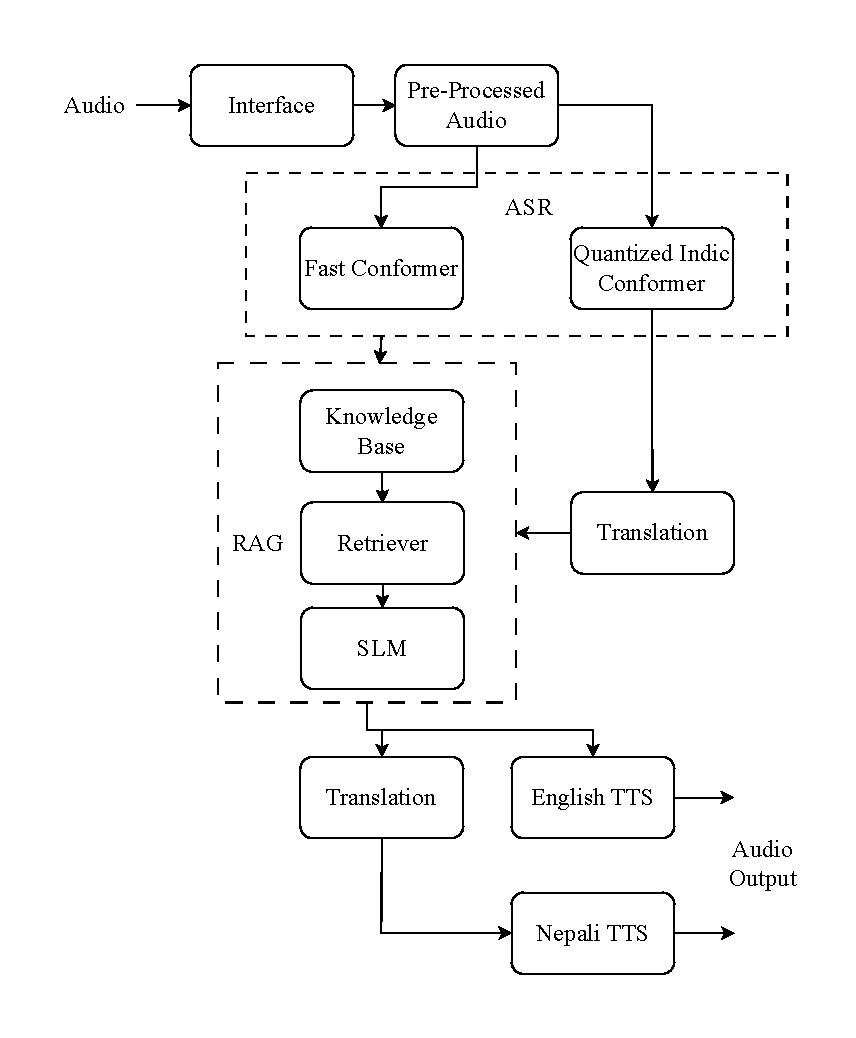
\includegraphics[width=\linewidth]{Images/ASR/Methodology/ASR-SuperMainArchitecture.drawio.pdf}
    \caption{System Architecture}
\end{figure}

The system pipeline starts with the spoken audio of the user that is either in English or Nepali. The Interface module handles the preprocessing of the audio signal after which it is sent to the relevant Automatic Speech Recognition (ASR) pathway depending on which language is being used.In the case of Nepali audio input, the signal is run through the Quantized Indic Conformer model that caters to Indic language meaning that the speech is converted into textual transcription. This transcription is further sent to a Translation module so that it can be translated to English before being sent to the Small Language Model (SLM).With English audio input, the signal is handled in a quicker pathway by the Fast Conformer model that directly transcribes the speech into text. This is an English transcription that is directly forwarded to the SLM without need of translation.The SLM also acts on a Retrieval-Augmented Generation (RAG) basis. It has a Knowledge Base which has the news articles and information of the last two years. When a transcribed text is received by the SLM, the Retriever component is used in a search of this Knowledge Base to retrieve information that is relevant and up-to-date concerning the query made by the user. This memory context is then subjected to the language interpretation abilities of the SLM to create correct responses of context-aware nature based on the latest news and events. The output of the SLM, which is refined on a specialized dataset and optimized to perform local inference, is the combination of the query input and the knowledge retrieved to produce a coherent reply in English.At the end, two output paths are available to the English text response: one of them is to send the English text response straight to the English TTS module and to receive the audio in English and another is to translate the SLM output to nepali and send it to the Nepali TTS module and to get the audio in Nepali. This two-way mechanism offers the system the ability to support bilingual input and offer versatile multilingual output as per the needs of the user.


\subsection{Automatic Speech Recognition}
\subsubsection{Architecture of ASR}
\begin{figure}[H]
    \centering
    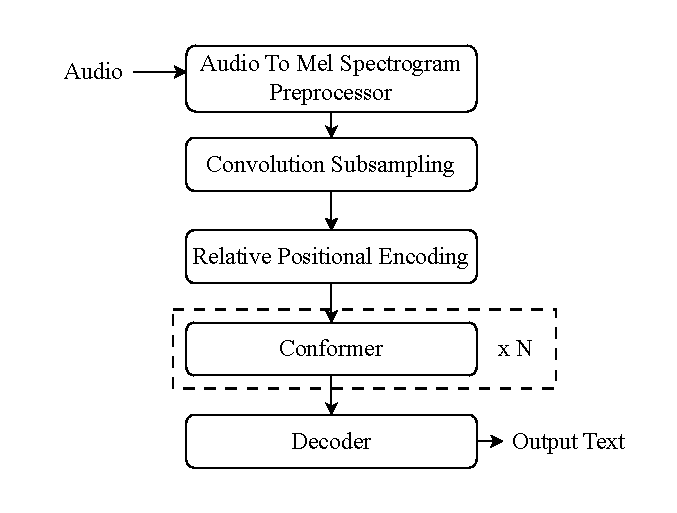
\includegraphics[width=\linewidth]{Images/ASR/Methodology/ASR-Main Architecture.drawio.pdf}
    \caption{Architecture of ASR}
\end{figure}
The ASR subsystem uses two different Conformer-based models to process english and nepali speech input. The FastConformer architecture based on EncDecCTCModelBPE is used to process English speech and the IndicConformer architecture based on EncDecHybridRNNTCTCBPEModel is used to process Nepali speech. Both models are also trained on NeMo benchmarks and have the same overall design, a convolutional front-end, a series of Conformer encoder layers, and a CTC decoding head, but have different model dimensionality, vocabulary size, and encoder layers, since they are trained on different scale data and linguistic complexity data.

\begin{table}[H]
\caption{Model Configuration Comparison: FastConformer (English) vs IndicConformer (Nepali)}
\label{tab:conformer_comparison}
\centering
\small
\begin{tabularx}{\textwidth}{|l|X|X|}
\hline
\textbf{Parameter} & \textbf{FastConformer (English)} & \textbf{IndicConformer (Nepali)} \\
\hline
Model class & \texttt{EncDecCTCModelBPE} & \shortstack[l]{\texttt{EncDecHybrid}\\\texttt{RNNTCTCBPEModel}} \\
Language & English & Nepali (Indic) \\
Encoder hidden dim & 176 & 512 \\
Encoder layers & 16 & 17 \\
FFN expansion ratio & $4\times$ (176 $\to$ 704) & $4\times$ (512 $\to$ 2048) \\
Conv kernel size (depthwise) & 31 & 31 \\
Attention dim & 176 & 512 \\
Vocabulary size & 1025 (BPE) & 5633 (BPE) \\
CTC projection & \texttt{Conv1d(176, 1025)} & \texttt{Conv1d(512, 5633)} \\
Decoding path used & CTC & CTC only \\
\hline
\end{tabularx}
\end{table}

\subsubsection{Feature Extraction}
Both models have the same front end preprocessing pipeline that is an AudioToMelSpectrogramPreprocessor using a FilterbankFeatures featurizer. The raw audio waveforms are converted into mel-frequency filterbank features and these features are then sent to the encoder. Both models use the same technique of the preprocessing pipeline since both are trained on 16 kHz speech data.

\textbf{Sampling Rate}\\
Audio input is resampled to a standard rate of 16,000 Hz (16 kHz) before the extraction of features. This provides consistency in training as well as inference. The frequency range of human speech has most of the perceptually important information in the range of frequencies up to 8 kHz. The Nyquist theorem states that at least 2 x 8,000 = 16,000 samples per second must be used to reproduce frequencies up to 8 kHz with perfect accuracy. 

\textbf{Windowing}
\begin{itemize}
    \item Window Size (25ms)\\
    This defines the time of every frame of time used to calculate spectral features. A 25 ms window provides enough temporal information for speech without at the same time being too local (i.e. less than 25 ms).
    \item Stride \\
    The hop length of 10 ms allows for overlapping frames, which ensures smooth transitions between consecutive feature vectors, capturing fine temporal details.
\end{itemize}

\textbf{Mel-Frequency Features (80 Bin)}
\begin{itemize}
    \item Extracting 80 mel-frequency features allows for a small size yet expressive representation of the audio signal focusing on perceptually relevant frequencies for human speech.
    \item The number of bins balances between resolution and model complexity.
\end{itemize}

\textbf{Logarithmic Scaling}
\begin{itemize}
    \item Applying a logarithmic transformation to the mel-spectrogram simulates the human auditory system's detection of sound intensity, which makes the features more meaningful for ASR models.
    \item This has the additional advantage of reducing problems with dynamic range in the spectrogram.
\end{itemize}

\textbf{Dithering}
\begin{itemize}
    \item Adding small random noise helps to avoid numerical instability in computations - especially if one is working with very small values or zero-padding in the spectrogram.
\end{itemize}

\subsubsection{Spectrogram Augmentation}
Both models apply spectrogram augmentation during training through a SpectrogramAugmentation module. The English FastConformer uses SpecAugment, while the IndicConformer uses both SpecAugment and SpecAugmentNumba — a GPU-accelerated implementation of the same algorithm. Spectrogram augmentation is applied only during training and is disabled at inference time. Two augmentation strategies are applied:

\begin{itemize}
\item \textbf{Time masking}: sequential time intervals in the mel spectrogram are initialised to zero. This imitates time-based acoustic dropouts in the form of momentary silence or other noise momentarily which causes the model to learn representations that are not dependable on either a time segment.

\item \textbf{Frequency masking}: Mel spectrogram frequency channels next to each other are set to zero. This makes it so that the model will not be dependent on a specific frequency band and its resistance to spectral distortion, channel mismatch, and varying background noise properties.
\end{itemize}

Combined, these masking techniques ensure that the Conformer encoder does not overfit itself to certain acoustic patterns within the training set, increasing generalisation to variable speaking rates, recording conditions and microphone properties.


\subsubsection{Convolutional Subsampling}
A ConvSubsampling module is used before a layer of Conformer encoder modules receives the mel-spectrogram features. Extracted raw mel spectrograms at a 10 ms frame shift result in very long input sequences, i.e. a 10s utterance generates 1,000 frames, that are computationally expensive to the self-attention mechanism in the Conformer, whose complexity increases with sequence length. The  convolutional subsampling step downsamples the input by 4 times in time, and this results in the encoder being much more efficient with no critical acoustical data loss.

Subsampling module is composed of two consecutive layers of Conv2d, and they have 3x3 kernel size and stride 2x2, and then ReLU activations. The consecutive stride-2 operations simultaneously reduce the time dimension by 4 times a sequence of 10 ms per frame is reduced to 20 ms per frame with the first convolution, and 40 ms per frame with the second. This resolution (40 ms/frame) is good enough to recognize speech at the phoneme level since the 10 ms time window of two adjacent frames is well correlated and has much redundant acoustic data.

The specific configurations for the two models are as follows:

\begin{table}[H]
\caption{ConvSubsampling layer dimensions}
\label{tab:convsubsampling_dimensions}
\centering
\begin{tabularx}{\textwidth}{|l|X|X|}
\hline
\textbf{Parameter} & \textbf{Fast Conformer} & \textbf{Indic Conformer} \\
\hline
Conv layer 1 & Conv2d(1, 176, 3$\times$3, stride 2) & Conv2d(1, 512, 3$\times$3, stride 2) \\
Activation 1 & ReLU & ReLU \\
Conv layer 2 & Conv2d(176, 176, 3$\times$3, stride 2) & Conv2d(512, 512, 3$\times$3, stride 2) \\
Activation 2 & ReLU & ReLU \\
Temporal reduction & 4$\times$ (10 ms $\to$ 40 ms) & 4$\times$ (10 ms $\to$ 40 ms) \\
\hline
\end{tabularx}
\end{table}

\subsubsection{Linear}

Conformer uses a linear layer in the model after the first process of convolutional subsampling to map the newly subsampled features into a larger space. This step is required because it brings the feature dimensions to the size of the hidden layers used by Transformer and convolutional modules. To explain this, the linear block picks the results from the downsampling, which lowers the time resolution and extracts local details, and completes the process by adding an extra layer to increase its dimensions. Doing this makes sure the achieved representation is able to hold detailed acoustic details and blends well with the self-attention and feed-forward modules from the Conformer design. This kind of design gives a balance between performance and calculations, helping the Conformer perform well in speech recognition.The convolutional front-end has this linear projection to guarantee that the output of each Conformer layer can be dimensionally compatible with the self-attention and feed-forward modules.

\begin{itemize}
    \item \textbf{Fast Conformer(English)}: Linear(in\_features=3520, out\_features=176). The 3520-dimensional input is the product of the 176-channel convolutional output and the frequency dimension after two stride-2 operations on 80 mel bins (80 / 4 = 20 frequency bins × 176 channels = 3,520). The output is a 176-dimensional embedding.

    \item \textbf{Indic Conformer(Nepali)}: Linear(in\_features=10240, out\_features=512). The 10240-dimensional input comes from 512 convolutional channels × 20 frequency bins. The output is a 512-dimensional embedding aligned with the Conformer encoder's model dimension.
\end{itemize}

\subsubsection{Dropout}

The dropout layer is put in place after the linear transformation that occurs after convolutional subsampling. This is very significant as it helps the model avoid complications during training. It reports that, by setting a percentage of the input tensor to zero randomly, dropout helps the learning process become a bit random. For this reason, the model must use all kinds of inputs, forming robust and generalized acoustic representations. This way of controlling overfitting matters, because speech data has many dimensions and the Conformer model includes both convolution and Transformers. Applying dropout in training guarantees steady and effective results for big speech recognition systems.

In the inference part, dropout is not utilized, so the model can use all its data to make predictions. Combining dropout with the Conformer’s design approach lets the architecture handle both performance and generalization to reach excellent results in automatic speech recognition

\subsubsection{Conformer Encoder}
\textbf{Conformer Architecture}
    \begin{figure}[H]
        \centering
        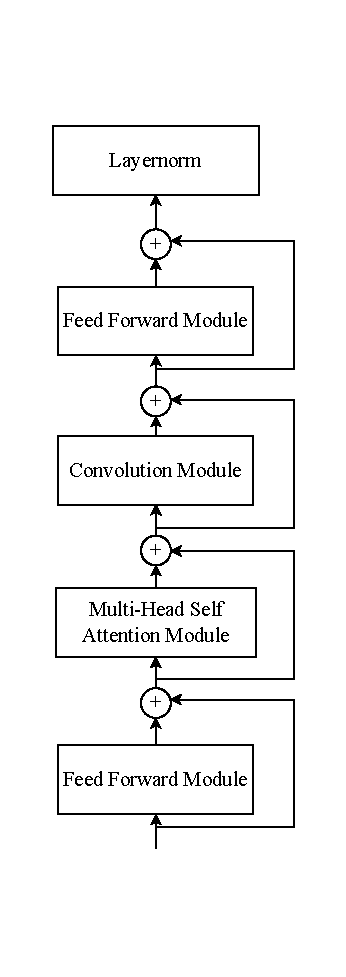
\includegraphics[scale=1]{Images/ASR/Methodology/ASR-ConformerBlock.drawio.pdf}
        \caption{Conformer Architecture}
    \end{figure}
The acoustic modelling element of the two ASR systems is the Conformer encoder. It works by stacking several of the same ConformerLayer blocks and each block is an assembly of multi-headed self-attention and local convolutional processing in a sandwich structure of macaron nets. FastConformer encoder employs 16 layers and the model dimension is 176 whereas IndicConformer encoder employs 17 layers and its model dimension is 512. Each layer has the same structure, and it is just the size that is different.

Every ConformerLayer has five sub-modules used in sequence, where first Feed Forward Module (FFN1), a Multi-Headed Self-Attention Module (MHSA), a Convolution Module (Conv), a second Feed Forward Module (FFN2), and a final Layer Normalisation. This structure, based on Macaron-Net, encircles the attention and convolution modules between two half-weighted feed-forward modules enabling the model to detect both regional and global speech patterns in a combined expression.

\textbf{Feed Forward Module}

The Conformer architecture requires the Feed Forward Module to deal with features at single-token level. It includes two FFNs that work in the same way, one before and one after the focus on attention and convolutional techniques. They function as processes before and after training to boost the model’s ability to learn features and still use few resources. All FFNs include certain layers in their structure: layer normalization, transformations, activation, and residual connections.

All FFNs start off with layer normalization , ensuring that the mean and variance of the input are stable. In doing this step, the inputs to the next layers become more controlled, making the whole training process more stable. Once the module is normalized, it goes on to use a linear transformation followed by a non-linear GeLU or ReLU function. This way, the model can represent situations that are not simple, but more complex. After the activation, the results are passed through a linear layer that reshapes them to the original number of features. To sum up, residual connections enable gradients to continue, making sure issues like vanishing gradients are not a problem during training.

\textbf{Multi-Headed Self Attention Module}

    \begin{figure}[H]
        \centering
        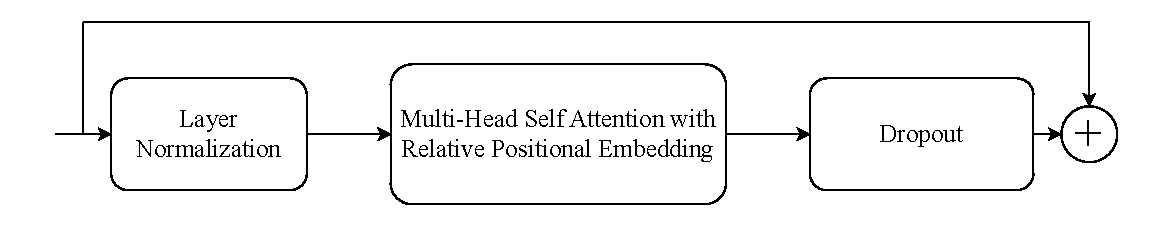
\includegraphics[width=\linewidth]{Images/ASR/Methodology/ASR-MultiHeadedSelfAttentionModule.drawio.pdf}
        \caption{Block Diagram of Multi-Headed Self Attention Module Architecture}
    \end{figure}

\textbf{Multi-Head Self Attention with Relative Positional Embedding}

    \begin{figure}[H]
        \centering
        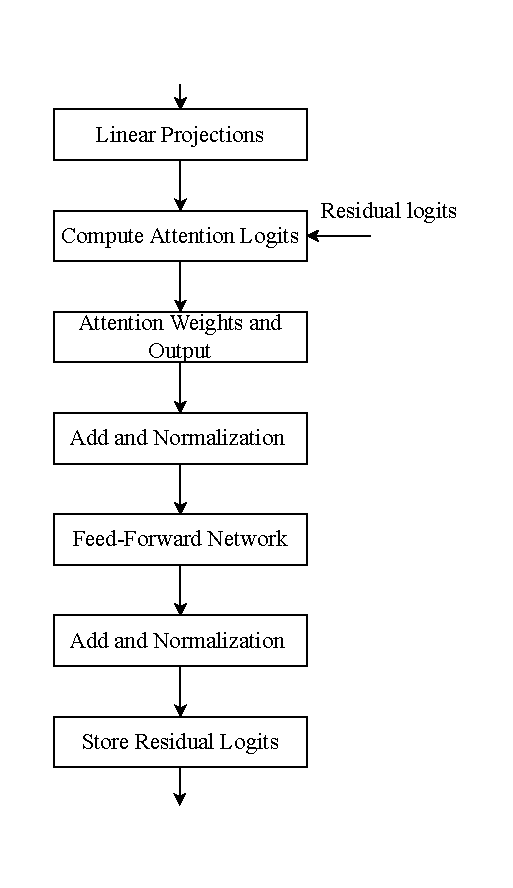
\includegraphics[scale=1]{Images/ASR/Methodology/ASR-ResMHA.drawio.pdf}
        \caption{Block Diagram of Multi-Head Self Attention with Relative Positional Embedding}
    \end{figure}
The self-attention sub-module gives attention to the long distance relationships in the entire sequence of the speech. It employs Relative Position Multi-Head Attention, which adds relative positional encoding to the attention score computation instead of appending some fixed absolute positional encoding to the input. This enables the model to extrapolate to utterances of varying lengths and also to be sensitive to the relative position of the frames instead of the absolute position of the frame within the sequence.
There are four known linear projections in the attention module which include query (Q), key (K), value (V) and output that all take place in the hidden dimension of the model. One more linear projection (linear\_pos) gives positional bias terms utilized in the calculation of the relative attention score. The attention weights are dropped (p=0.1). Layer Normalization comes before the module. The specific dimensions are:
\begin{itemize}
    \item \textbf{Fast Conformer(English)}:  All projections are Linear(176, 176). With a model dimension of 176 and 4 attention heads, each head operates over a 44-dimensional subspace.

    \item \textbf{Indic Conformer(Nepali)}: All projections are Linear(512, 512). With a model dimension of 512 and 8 attention heads, each head operates over a 64-dimensional subspace.
\end{itemize}
 
\textbf{Convolution Module}
    \begin{figure}[H]
        \centering
        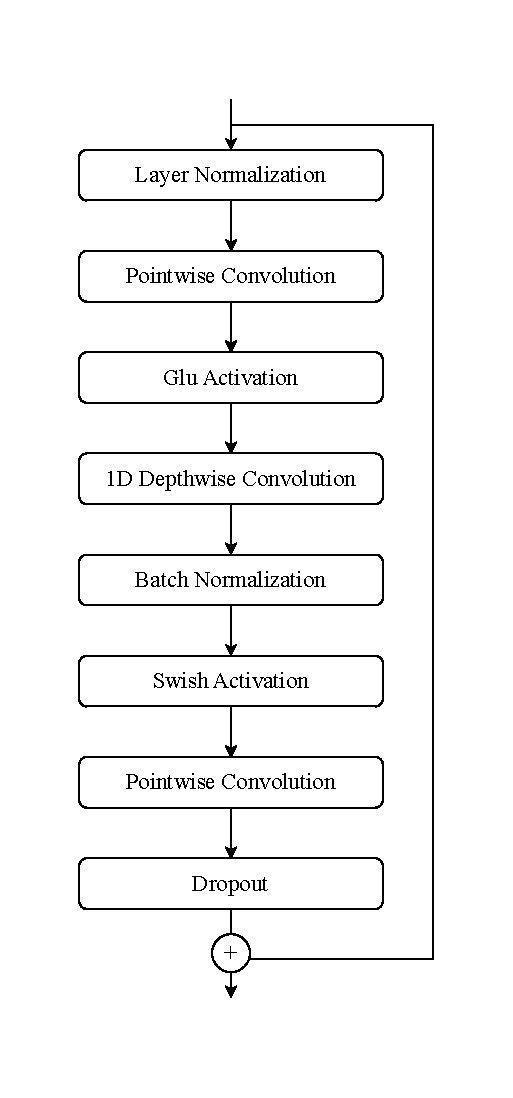
\includegraphics[scale=1]{Images/ASR/Methodology/ASR-Convolution Module.drawio.pdf}
        \caption{Block Diagram of Convolution Module}
    \end{figure}
    \begin{enumerate}
        \item \textbf{Pointwise Convolution}

        Part of the convolutional modules makes use of pointwise convolution to reorganize feature representations efficiently. A pointwise convolution also known as 1x1 convolution works by running a convolutional filter over all input channels with a kernel size of 1. In Conformer, time is what is being transformed in the temporal dimension of the speech features. One of the main uses of pointwise convolution is to keep the input’s spatial or temporal features while transforming it to a different dimension. 
        
        With pointwise convolutions, the Conformer saves computations and improves model performance, since it skips costly spatial computations.

        \item \textbf{GLU Activation}

        The GLU activation function is added to bring non-linearity and make the features better represented. The input is separated into two pieces, and the “gate” part gets processed by a sigmoid function, then those values are multiplied with the remaining data. Because of gating, the model can control information being exchanged and give more attention to significant elements as needed. By using GLU on the feed-forward and convolutional layers in the Conformer increases the ability to represent speech data while maintaining a good balance between simplicity and complexity.

        \begin{figure}[H]
            \centering
            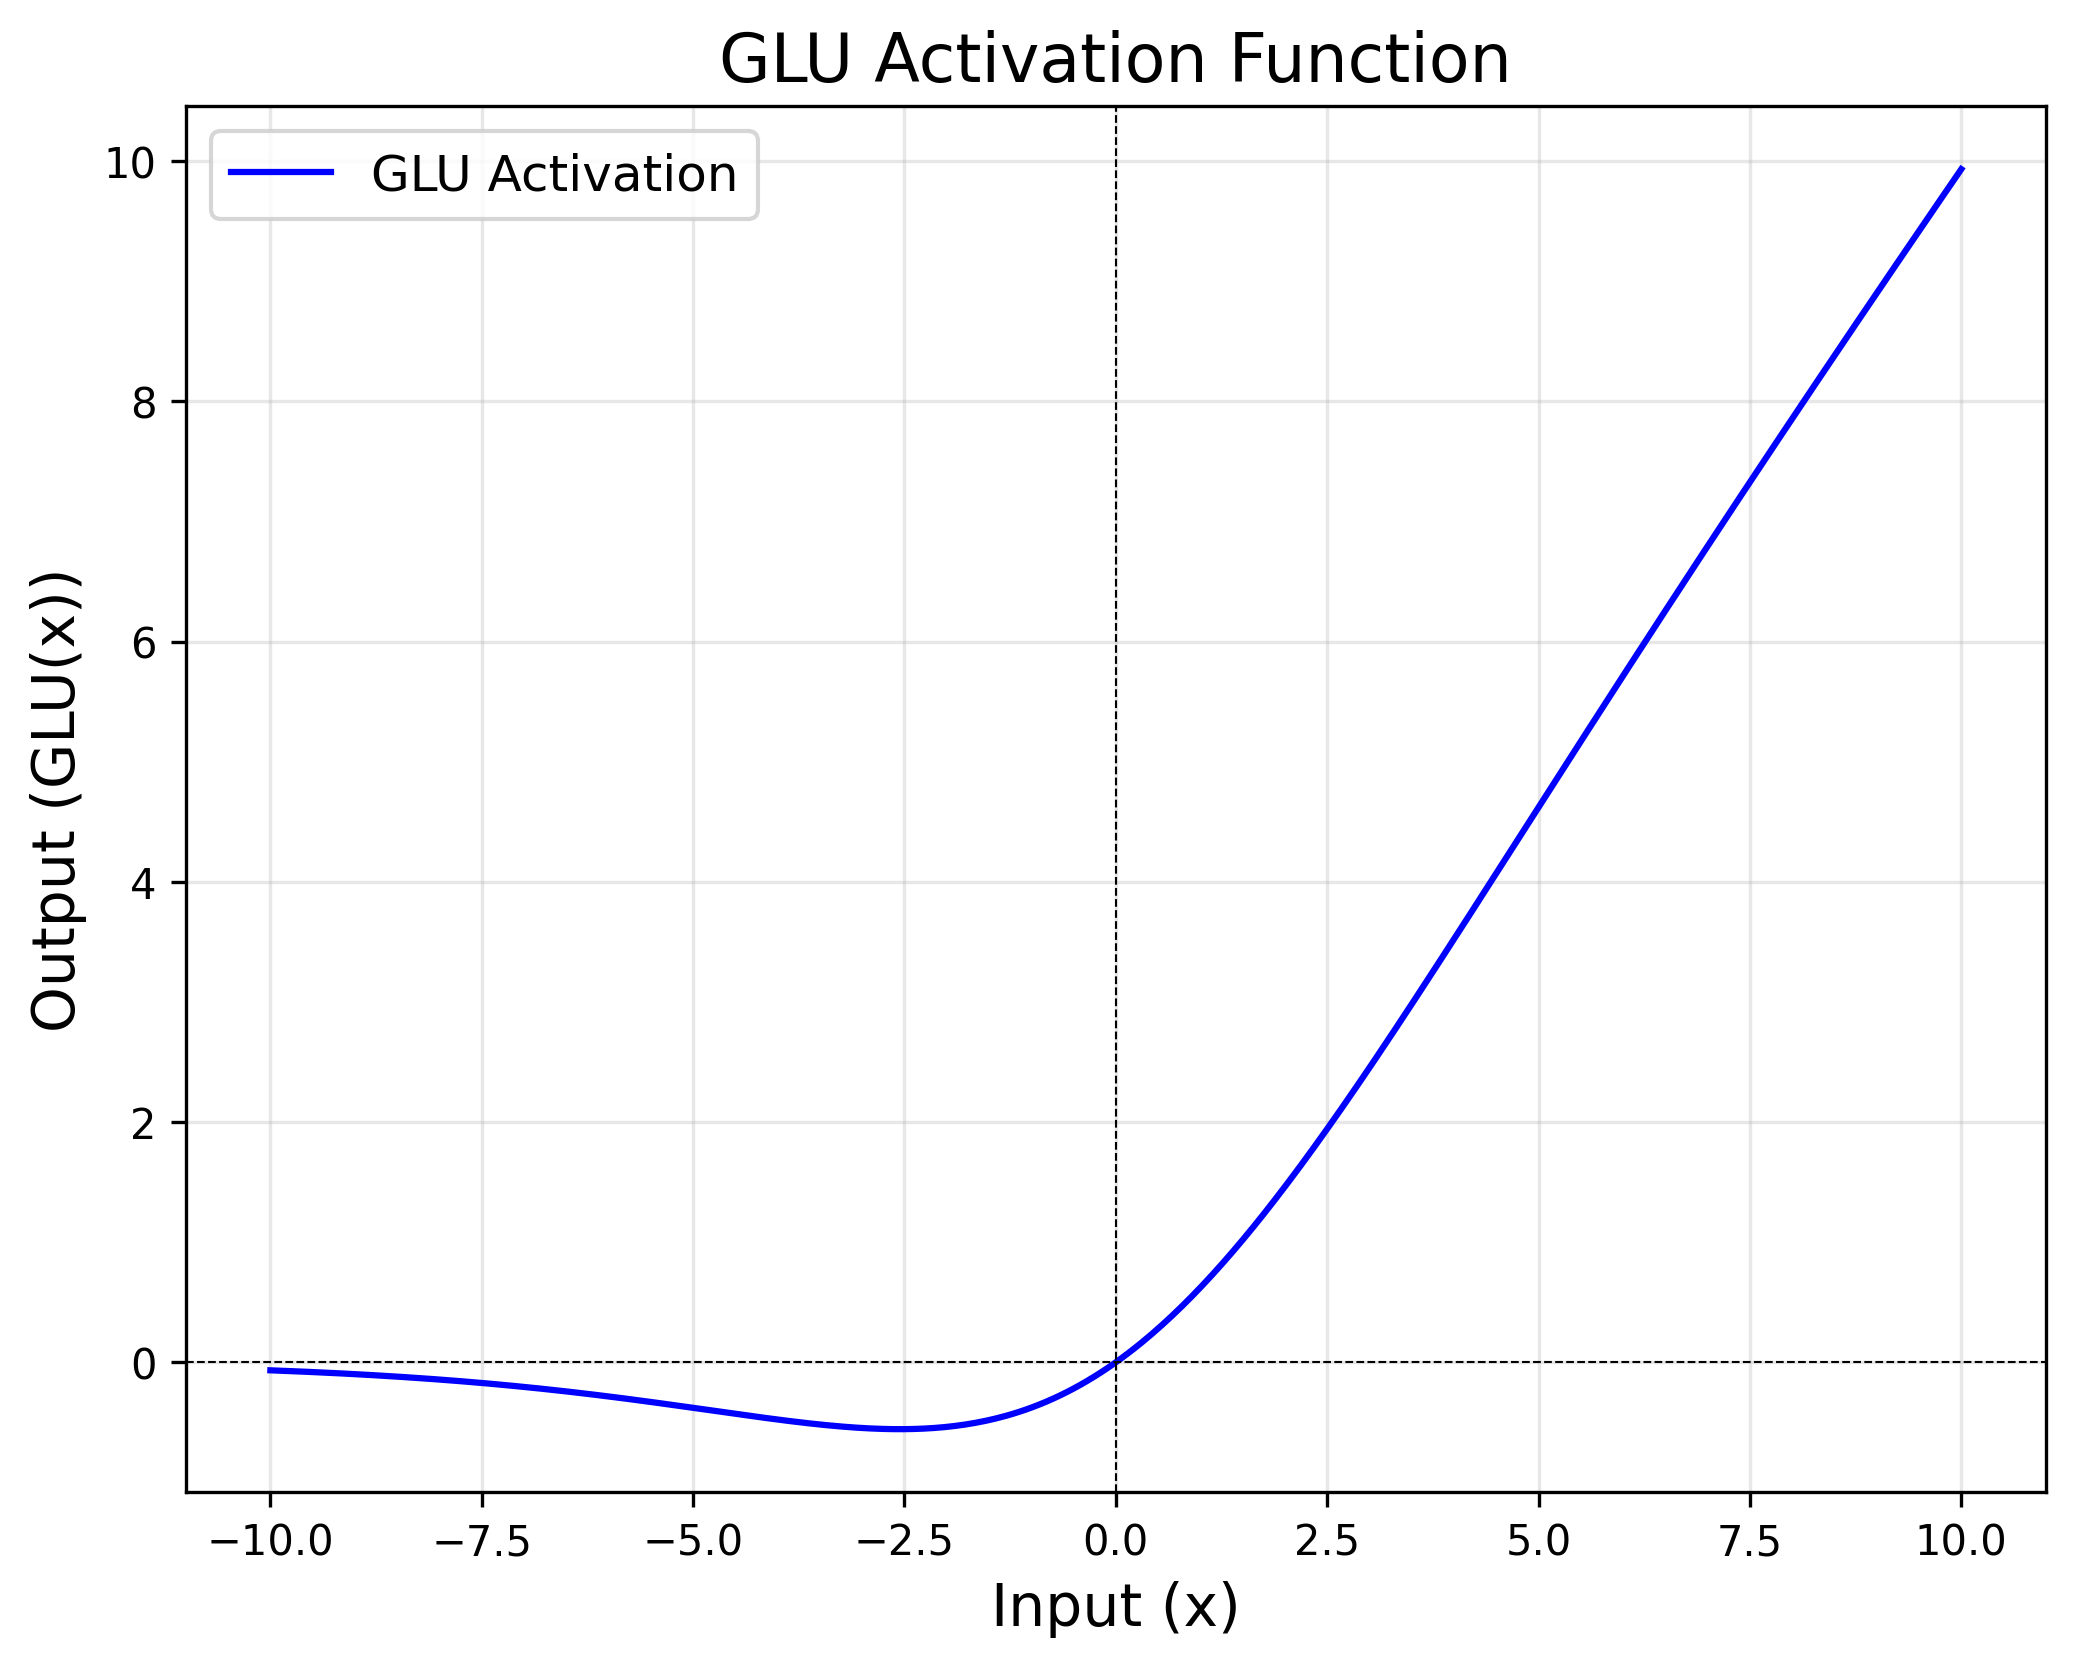
\includegraphics[width=\linewidth]{Images/ASR/Methodology/glu_activation.png}
            \caption{Graph of GLU activation}
        \end{figure}
        
        \begin{figure}[H]
            \centering
            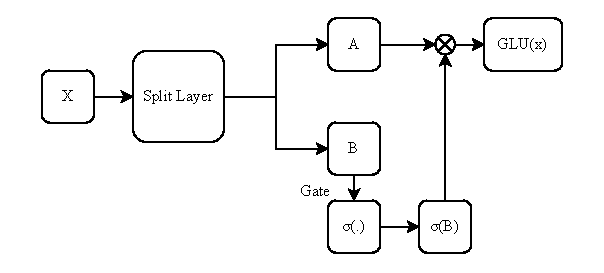
\includegraphics[width=\linewidth]{Images/ASR/Methodology/ASR-GLU.drawio.pdf}
            \caption{Block Diagram of GLU activation}
        \end{figure}
        
        
        \item \textbf{1D depthwise convolution}

        The Conformer designs 1D depthwise convolution to catch the connections between parts of speech by filtering each channel in sequence along the time axis. Consequently, resources are saved without losing the following local features. It combines pointwise convolution to help channels connect, thus it works well for modeling features in successive speech.

        \item \textbf{Swish Activation}

        The Swish activation function is well known in deep learning since it performs better than simpler activation functions like ReLU (Rectified Linear Unit). Swish is useful in the Conformer architecture because it boosts both the strength and speed of training for automatic speech recognition tasks.
        Swish is defined as:
        \begin{equation}
            \text{Swish}(x) = x \cdot \sigma(x)
        \end{equation}

        \begin{figure}[H]
            \centering
            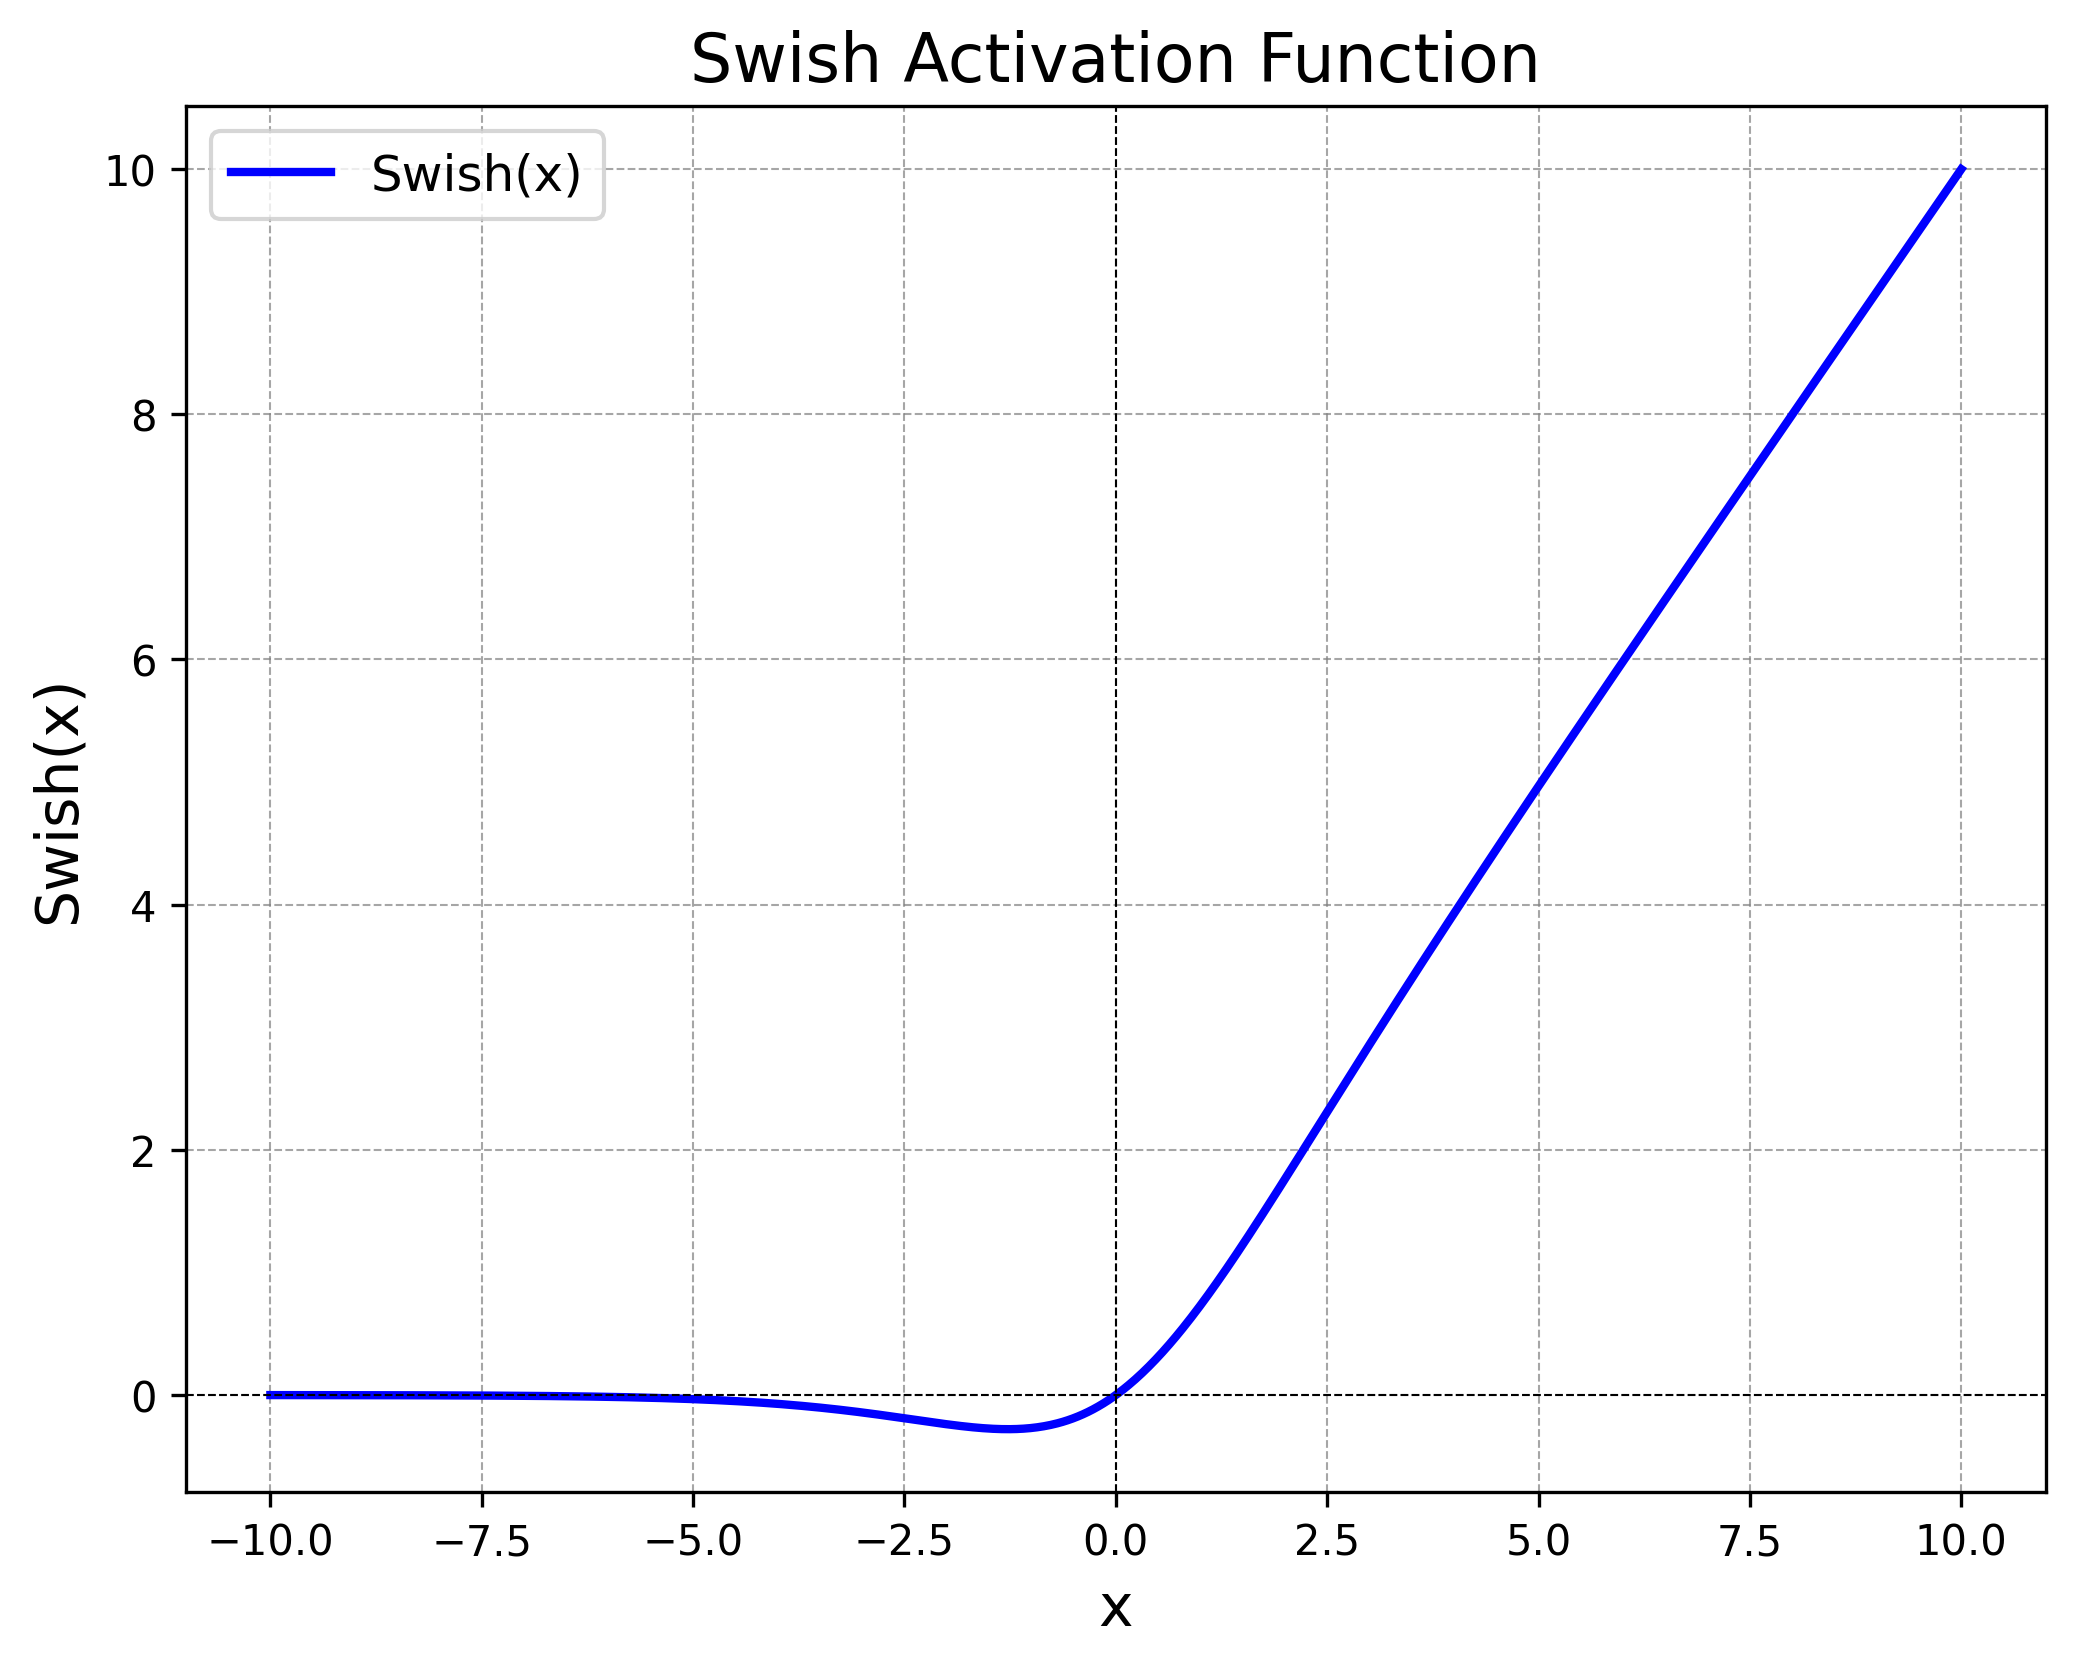
\includegraphics[width=\linewidth]{Images/ASR/Methodology/swish_activation.png}
            \caption{Graph of Swish Activation} \end{figure}
    \end{enumerate}
    
\textbf{Layer Normalization}\\
The purpose of Layer Normalization is to keep the training stable and speedy by normalizing the activations in all layers. To be clear, it standardizes each input value in every feature dimension (the hidden dimension) for each step. This lets the mean and variance of the activations not change, so problems with vanishing or exploding gradients are avoided. It is applied in many places in the network to make sure the gradients do not experience fluctuations. As internal covariate shift is limited, the model performs better at obtaining strong features from speech data, seen mainly in deep networks with lots of layers. This method becomes crucial for reaching consistent and efficient convergence in automatic speech recognition. 

\textbf{Conformer Block Computation}\\
Our proposal for Conformer includes putting the Multi-Headed Self-Attention and the Convolution modules between two Feed Forward modules. Macaron-Net \cite{macaron} was a motivation behind this sandwich structure, and it suggests removing the regular feed-forward layer from a normal Transformer block and placing two reduced-size feed-forward layers, one before and another after the attention layer. Like in Macron-Net, we add half-step residual weights to the feed-forward (FFN) parts of our model. The second feed-forward module comes ahead of the last layernorm layer. In math terms, yi is the output produced by Conformer block i as it takes input xi as input.
     
Mathematically, this means that for input $x_i$ to a Conformer block $i$, the output $y_i$ of the block is:
    \begin{align}
    \tilde{x}_i &= x_i + \frac{1}{2} \text{FFN}(x_i) \\
    x'_i &= \tilde{x}_i + \text{MHSA}(\tilde{x}_i) \\
    x''_i &= x'_i + \text{Conv}(x'_i) \\
    y_i &= \text{LayerNorm}\left(x''_i + \frac{1}{2} \text{FFN}(x''_i)\right)
    \end{align}

\subsubsection{SentencePiece Tokenizer}
Sentence Piece is a language-neutral subword tokenisation system that is actively used in end-to-end automatic speech recognition (ASR) systems to alleviate vocabulary sparsity and out-of-vocabulary (OOV) effects. SentencePiece is unlike tokenisers, which rely on whitespace, and works on an unsegmented stream of Unicode characters, where subword units are directly learned from the input. It is therefore especially beneficial when dealing with languages that do not have clear word delimiting boundaries and with infrequent or misspelt words in speech transcripts. The framework incorporates the use of either the Byte-Pair Encoding (BPE) as the base algorithms and thus enables one to trade-off the granularity of tokens and the general model performance. SentencePiece produces strong, compact representations, operating on a subset of corpora coded uniformly and reversibly into subword tokens, such as special symbols marking the start and end of an utterance, and these representations are compatible with the output of acoustic models in modern ASR pipelines.

\begin{algorithm}[H]
	\caption{Train SentencePiece Tokenizer (BPE)}
	
	\textbf{Input:} Raw training text, target vocabulary size, model type (BPE), special tokens \\
	\textbf{Output:} Trained tokenizer model, subword vocabulary, encoding and decoding rules
	
	1. Preprocess the training text by normalizing whitespace and optionally adding sentence boundary markers\;
	
	2. Initialize a character-level vocabulary using all unique Unicode symbols present in the text\;
	
	3. Add predefined special tokens (e.g., \texttt{<s>}, \texttt{</s>}, \texttt{<unk>}) to the vocabulary\;
	
	4. If the model type is BPE:
	\begin{itemize}
		\item Initialize all characters as individual tokens
		\item Convert the full text into a sequence of tokens based on the current vocabulary
		\item Repeat until the target vocabulary size is reached:
		\begin{itemize}
			\item Count the frequency of all adjacent token pairs
			\item Select the most frequent token pair
			\item Merge the selected pair into a new subword token
			\item Add the new token to the vocabulary
			\item Replace all occurrences of the merged pair in the token sequence
		\end{itemize}
	\end{itemize}
	
	5. Save the learned vocabulary, subword merge rules, and model parameters\;
	
	6. Return the trained tokenizer capable of encoding and decoding arbitrary text sequences\;
	
\end{algorithm}

\subsubsection{Connectionist Temporal Classification (CTC) Head}

Connectionist Temporal Classification (CTC) is commonly used in sequence-to-sequence
tasks such as speech recognition and handwriting recognition, where the input and
output sequences are of different lengths and are not pre-aligned. CTC can be used
both as a loss function during training and as a decoding strategy during inference.

CTC introduces a special \emph{blank symbol}, typically denoted as \( b \), which
allows the model to emit either an output symbol \( y_t \) or a blank at each time
step of the input sequence.

Let the input sequence be
\begin{equation}
	\mathbf{x} = (x_1, x_2, x_3, \dots, x_T),
\end{equation}
where \( T \) denotes the input sequence length, and let
\begin{equation}
	\mathbf{y} = (y_1, y_2, \dots, y_U)
\end{equation}
be the target output sequence.

CTC defines a collapsing function \( \mathcal{B} \) that removes repeated symbols
and blank symbols. The set of all alignment paths that collapse to \( \mathbf{y} \)
is denoted by
\begin{equation}
	\mathcal{B}^{-1}(\mathbf{y}).
\end{equation}
\begin{itemize}
    \item \textbf{Fast Conformer(English)}: Conv1d(176, 1025, kernel size=1). Projects the 176-dimensional encoder output to a 1025-token vocabulary (1024 BPE subword units + 1 blank token).

    \item \textbf{Indic Conformer(Nepali)}: Conv1d(512, 5633, kernel size=1). Projects the 512-dimensional encoder output to a 5633-token vocabulary (5632 BPE subword units + 1 blank token, with padding\_idx=5632).
\end{itemize}

\textbf{CTC Objective}

The conditional probability of the output sequence \( \mathbf{y} \) given the input
sequence \( \mathbf{x} \) is defined as
\begin{equation}
	P(\mathbf{y} \mid \mathbf{x}) =
	\sum_{\boldsymbol{\pi} \in \mathcal{B}^{-1}(\mathbf{y})}
	P(\boldsymbol{\pi} \mid \mathbf{x}),
\end{equation}
where \( \boldsymbol{\pi} = (\pi_1, \pi_2, \dots, \pi_T) \) represents an alignment path.

Each alignment probability is factorized over time steps as
\begin{equation}
	P(\boldsymbol{\pi} \mid \mathbf{x}) =
	\prod_{t=1}^{T} P(\pi_t \mid \mathbf{x}),
\end{equation}
with
\begin{equation}
	\pi_t \in \mathcal{Y} \cup \{ b \},
\end{equation}
where \( \mathcal{Y} \) is the output vocabulary and \( b \) denotes the blank symbol.

The summation over all valid alignments is efficiently computed using dynamic
programming techniques such as the forward--backward algorithm.

\textbf{Inference}

During inference, the output sequence is simplified by collapsing consecutive
repeated symbols and removing blank symbols. For example,
\begin{equation}
	\texttt{h\_l\_l\_o} \;\longrightarrow\; \texttt{hello}.
\end{equation}

\textbf{Comparison with Attention-Based Methods}

Unlike attention-based models that perform global alignment between input and output
sequences, CTC performs alignment locally at each time step. This local alignment
strategy avoids scanning the entire sequence during decoding, leading to improved
computational efficiency, especially for long input sequences.

\subsubsection{AdamW Optimizer}
AdamW is an improvement over the traditional Adam optimizer, as it decouples the
weight decay term from the gradient-based parameter updates, thereby enabling more
effective regularization. This property is particularly beneficial when training
large-scale deep learning models such as FastConformer, a highly efficient variant
of the Conformer architecture used in speech recognition.

In the standard Adam formulation, weight decay is applied through L2 regularization
of the loss, which can interfere with the adaptive learning-rate mechanism. AdamW
addresses this limitation by applying weight decay directly to the model parameters
after the Adam update step, as shown in the following equation:

\begin{equation}
	\theta_{t+1} = \theta_t
	- \eta \left( \frac{\hat{m}_t}{\sqrt{\hat{v}_t} + \epsilon} \right)
	- \eta \lambda \theta_t
\end{equation}

where \( \theta_t \) represents the model parameters at training step \( t \),
\( \eta \) is the learning rate, \( \hat{m}_t \) and \( \hat{v}_t \) are the
bias-corrected first and second moment estimates, respectively, and \( \lambda \)
denotes the weight decay coefficient.

In architectures such as FastConformer, which combine convolutional and
self-attention layers, training stability and generalization are critical. By
providing cleaner and more consistent regularization, AdamW typically leads to
better convergence behavior and improved generalization compared to the standard
Adam optimizer, especially when training transformer-based models with large batch
sizes and long input sequences.

\subsubsection{Cosine Annealing}
Cosine annealing is a non-linear learning rate-scheduling method, common in fine-tuning deep neural networks, and widely used to fine-tune pre-trained models of speech recognition, such as FastConformer. As compared to aggressive decay schemes, cosine annealing progressively decreases the learning rate according to a cosine curve, beneficial to maintaining knowledge acquired in the pre-trained weights but enabling a controlled adaptation to the target domain.
In the case of fine-tuning, the model parameters are already in a well-trained state (e.g. using large-scale training data, such as LibriSpeech). Any initial learning rate can be catastrophically forgetful or unstable, and a fixed low initial learning rate can result in underfitting. Cosine annealing is one way to solve this problem, with an initial small learning rate gradually reduced towards zero during the fine-tuning.

\begin{equation}
\eta_t
=
\eta_{\min}
+
\frac{1}{2}
\left(\eta_{\max} - \eta_{\min}\right)
\left(
1 + \cos\left(\frac{\pi t}{T}\right)
\right)
\end{equation}

\begin{itemize}
  \item $\eta_t$: learning rate at step or epoch $t$
  \item $\eta_{\max}$: initial (maximum) learning rate
  \item $\eta_{\min}$: minimum learning rate
  \item $t$: current step or epoch, $0 \leq t \leq T$
  \item $T$: total number of steps or epochs
\end{itemize}

\subsubsection{Greedy Decoding}
Greedy batch decoding which is an efficient inference strategy is used to perform transcription which is typically used in Connectionist Temporal Classification (CTC) based Automatic Speech Recognition (ASR) systems. Greedy decoding chooses the most likely token at a time step without one looking at other hypotheses or context. This process can be optimized by the so-called batch (greedy\_batch) variant, which applies parallelized decoding of many audio samples but in that instance to one file with batch\_size=1 to be compatible and to have slight efficiency improvements.
Greedy decoding, in contrast to more advanced approaches like beam search, does not have a pool of candidate sequences, and thus is unable to combine external knowledge such as language models. It consequently can achieve low latency and high performance, but can result in lower fluent or grammatically irregular outputs, notably under noisy environments, or on ambivalent acoustic inputs. The method is based on the fact that the model (here a FastConformer) is only able to directly decode audio features into subword units (BPE tokens) and then decodes without rescoring or language improvement.
Therefore, it is a system that gives more focus to computational performance and simplicity than to the linguistic quality, so that it can be used in real-time-sensitive applications or in other situations where speed is paramount and minor mistakes in the transcription are tolerable.

\subsubsection{Softmax Function}
Softmax function helps convert raw logits from the output layer into a distribution of probabilities for the target vocabulary. This means the model creates probabilities for every output token (such as phonemes, characters or words) and, during decoding, it can pick the most likely sequence.

\begin{equation}
\text{softmax}(z_i) = \frac{e^{z_i}}{\sum_{j=1}^{K} e^{z_j}}
\end{equation}

\begin{itemize}
  \item \( z_i \): The input score (logit) for class \( i \)
  \item \( z_j \): The input score (logit) for class \( j \)
  \item \( K \): The total number of classes
\end{itemize}

\subsubsection{Word Error Rate (WER)}
Word Error Rate (WER) is the most popular metric used to evaluate the performance of the Automatic Speech Recognition (ASR) systems. It is used to measure the accuracy of transcription by comparing the hypothesis of the system to a ground-truth reference transcript.


\begin{equation}
	\text{WER} = \frac{S+D+I}{N}
\end{equation}

where,
\begin{itemize}
	\item S = Number of substitutions (wrong words)
	\item D = Number of deletions (missing words)
	\item I = Number of insertions (extra words)
	\item N = Total number of words in the reference
\end{itemize}

\input{Report/4_2_Methodology_SLM}
\input{Report/4_3_Methodology_RAG}
\newpage
\section{\MakeUppercase{Implementation Details}}
\subsection{ASR}
\subsubsection{Dataset Preperation}
The Automatic Speech Recognition (ASR) datasets are usually based on 16 kHz mono audio due to the effective tradeoff between speech intelligibility and computational efficiency. The 16 kHz sampling frequency, which is based on the Nyquist theorem, retrieves the frequencies up to 8 kHz- the range that is most important to the human voice- without introducing the high-frequency data that is not necessary and beneficial to the recognition performance as offered by higher rates such as 44.1 kHz. Also, mono (single-channel) audio is common in ASR systems since recognition is based on phonemes and time, and not space or direction; downmixing stereo audio to mono reduces memory space by half, makes preprocessing and model construction much easier, and does not lose speech content that is important. Combined, these decisions help to cut down on data size and computational load to support faster and more efficient model training and inference without compromising accuracy.

OpenSLR54, Librispeech100 and OpenSLR12 hosted the dataset which contained the nepali and English audio dataset. The dataset was split into training set, validation set and test set in an 85:10:5 in a data of 10 hours to make sure that there is enough data to be used in the model learning and still have smaller portions to be used in the evaluation and tuning. In an effort of enhancing the strength of the ASR model, noise augmentation was done on each split separately. In particular, each subset consisted of 50\% samples that were randomly selected and noised with the environment. The four categories used in drawing the noise included crowd, construction, traffic, and wind to recreate the acoustic conditions in the real world. The individual clean audio samples were then randomly cross-mixed with a noise segment of these categories using a controlled SNR-based method, so as to guarantee a consistent noise intensity across the dataset. The rest half of the data were retained clean to have a balance in terms of noisy and noise free samples. Through this strategy, the model is able to learn the optimal and negative listening conditions, hence improving its generalization and performance in the real world implementation situations.

The majority of our data was obtained by OpenSLR. The files and its description are contained in manifest. Every sample has a distinct identifier, the audio file path, audio transcription, type of noise, signal to noise ratio in decibels, and dataset division (train, validation, or test). This format is easy to access and filter and is therefore appropriate to use in tasks such as speech recognition in dissimilar acoustic environments. For the purpose of testing independently, We used Fleurs dataset which contains about 2.28 hours of audio data with its transcript. The Fleurs dataset contains the clean audio file and the well-structured transcript for the nepali language. All the audio files here were embedded with noise using scripts with the SNR level similar to the training dataset and the dataset was used specifically for the purpose of testing our model.


\subsubsection{FastConformer-CTC-BPE}

\textbf{Model Architecture and PEFT Configuration}

The NVIDIA NeMo FastConformer-CTC-BPE model was used as the base automatic speech recognition system in the experiments. The model follows an encoder-decoder architecture that uses Connectionist Temporal Classification (CTC) loss for sequence-to-sequence mapping. The encoder is a Conformer-based model with approximately ~ 13 million parameters, while the decoder is a convolutional ASR decoder with 181,000 parameters. The total number of parameters in the base model is 13,204,721.

To achieve parameter-efficient fine-tuning, the NeMo adapter-based PEFT architecture was used. This approach is supported by NeMo as an alternative to LoRA for Conformer-based architectures. Adapter modules were inserted only into the encoder component, while all other parameters were kept frozen during training. Each adapter used a linear bottleneck architecture under the configurations shown in Table~\ref{tab:fastconformer_adapter}. This design reduced the number of trainable parameters to only 50,688, which corresponds to 0.3839\% of the total model parameters.

\begin{table}[H]
\caption{Adapter Configuration Parameters}
\label{tab:fastconformer_adapter}
\centering
\begin{tabular}{|l|l|}
\hline
\textbf{Parameter} & \textbf{Configuration Value} \\
\hline
Target Module & Encoder \\
Adapter Dimension & 8 \\
Adapter Dropout & 0.25 \\
Activation Function & Swish \\
Normalization Position & Pre-norm \\
Input Feature Size & 176 \\
Trainable Parameters & 50,688 \\
Trainable Percentage & 0.3839\% \\
\hline
\end{tabular}
\end{table}

\textbf{Dataset and Preprocessing}

Training was conducted on a custom English ASR dataset written in NeMo manifest format and stored as JSONL files. The dataset was divided into training, validation, and test subsets. All audio samples were processed at a sampling rate of 16,000 Hz. Duration filtering was applied to remove utterances shorter than 0.5 seconds and longer than 20 seconds.

The data loader used seven worker processes with pinned memory enabled to improve GPU data transfer efficiency. Silence trimming was disabled in order to preserve natural speech characteristics. Table~\ref{tab:fastconformer_dataset} presents the statistical distribution of the dataset splits.

\begin{table}[H]
\caption{Dataset Split Statistics}
\label{tab:fastconformer_dataset}
\centering
\begin{tabular}{|l|l|l|l|}
\hline
\textbf{Split} & \textbf{Samples} & \textbf{Duration} & \textbf{Average Words} \\
\hline
Train & 4,859 & 17.03 hours & 35.26 \\
Validation & 571 & 1.99 hours & 35.26 \\
Test & 287 & 0.98 hours & 35.10 \\
\hline
\end{tabular}
\end{table}

\textbf{Training Configuration}

Training was performed using PyTorch Lightning together with the NeMo toolkit. Optimization was carried out using AdamW with decoupled weight decay. A cosine annealing scheduler was used to control the learning rate, together with a warmup phase to stabilize the initial training dynamics. bfloat16 mixed precision training was enabled to reduce memory usage and accelerate computation on the available GPU hardware. The training hyperparameters are summarized in Table~\ref{tab:fastconformer_train}.

\begin{table}[H]
\caption{Training Hyperparameters}
\label{tab:fastconformer_train}
\centering
\begin{tabular}{|l|l|}
\hline
\textbf{Parameter} & \textbf{Value} \\
\hline
Maximum Epochs & 15 \\
Train Batch Size & 32 \\
Validation Batch Size & 64 \\
Gradient Accumulation Steps & 2 \\
Learning Rate & $1\times10^{-4}$ \\
Minimum Learning Rate & $1\times10^{-6}$ \\
Weight Decay & $5\times10^{-2}$ \\
Adam Betas & (0.9, 0.98) \\
Warmup Ratio & 0.1 \\
Gradient Clipping & 1.0 \\
Precision & bf-16 mixed\\
Learning Rate Scheduler & Cosine Annealing \\
\hline
\end{tabular}
\end{table}

\textbf{Data Augmentation}

SpecAugment was applied during training to improve model robustness against acoustic variability. This augmentation strategy helps the model generalize better to unseen acoustic conditions by masking selected regions of the spectrogram. The frequency and time masking configurations are shown in Table~\ref{tab:fastconformer_aug}.

\begin{table}[H]
\caption{Data Augmentation Parameters}
\label{tab:fastconformer_aug}
\centering
\begin{tabular}{|l|l|l|}
\hline
\textbf{Augmentation Type} & \textbf{Count} & \textbf{Maximum Width} \\
\hline
Frequency Masks & 2 & 15 frequency bins \\
Time Masks & 6 & 30 time steps \\
\hline
\end{tabular}
\end{table}

\textbf{Regularization and Checkpointing}

Early stopping was based on validation Word Error Rate (WER) as the monitoring metric. Model checkpoints were saved at regular intervals, and the best-performing checkpoint was retained according to validation performance. This strategy helped reduce overfitting and ensured that the best model weights were preserved for final evaluation. The checkpointing and early stopping criteria are given in Table~\ref{tab:fastconformer_ckpt}.

\begin{table}[H]
\caption{Checkpoint and Early Stopping Configuration}
\label{tab:fastconformer_ckpt}
\centering
\begin{tabular}{|l|l|}
\hline
\textbf{Configuration} & \textbf{Value} \\
\hline
Monitor Metric & Validation WER \\
Mode & Minimization \\
Patience & 5 epochs \\
Minimum Delta & 0.001 \\
Save Top K & 1 \\
Checkpoint Frequency & Every 1 epoch \\
\hline
\end{tabular}
\end{table}

% intetionally commented out 

% \textbf{Software and Hardware Environment}

% A fixed software stack was used to ensure reproducibility of the implementation. All experiments were conducted on Google Colab using an NVIDIA Tesla T4 GPU. Deterministic training was enabled in warn-only mode to account for non-deterministic GPU CTC backward operations while maintaining reproducibility wherever possible. A random seed of 42 was used throughout the experiments. The software and hardware specifications are provided in Table~\ref{tab:fastconformer_env}.

% intetionally commented out 

% \begin{table}[H]
% \caption{Software and Hardware Configuration}
% \label{tab:fastconformer_env}
% \centering
% \begin{tabular}{|l|l|}
% \hline
% \textbf{Component} & \textbf{Version / Specification} \\
% \hline
% NVIDIA NeMo Toolkit & 2.4.0 \\
% PyTorch Lightning & $\geq$ 2.2.0, $<$ 2.6.0 \\
% Python & 3.12 \\
% CUDA & 12.8 \\
% NumPy & 1.26.4 \\
% GPU Accelerator & NVIDIA Tesla T4 \\
% Random Seed & 42 \\
% \hline
% \end{tabular}
% \end{table}

\textbf{Model Export and Checkpointing}

After training, the best model checkpoint was exported in multiple formats to support different deployment scenarios. The complete model was saved in NeMo format with full model weights for direct deployment. In addition, the adapter weights were saved separately in PyTorch format, containing only the trainable adapter parameters for efficient storage and transfer. This dual-export strategy supports both full-model deployment and adapter-only fine-tuning in resource-constrained environments.

\subsubsection{Implementation Details for Indic Conformer}

\textbf{Model Architecture and Configuration}

The automatic speech recognition system was built using the IndicConformer \texttt{stt\_ne\_conformer\_ctc\_rnnt\_large} variant. This model uses a hybrid loss function that combines Connectionist Temporal Classification (CTC) and Recurrent Neural Network Transducer (RNNT) objectives, allowing it to benefit from both alignment-free and sequence-to-sequence training paradigms.

The architecture consists of a Conformer-based encoder, an RNNT decoder, a joint network, and an additional CTC decoder head. The model uses a SentencePiece tokenizer with a vocabulary of 5,632 tokens, derived from 256 tokens per language unit. Unlike the FastConformer-CTC-BPE setup, all model parameters were fully fine-tuned, resulting in approximately 129 million trainable parameters. Table~\ref{tab:indic_model} summarizes the main architectural components and their parameter distribution.

\begin{table}[H]
\caption{Model Components and Parameter Distribution}
\label{tab:indic_model}
\centering
\begin{tabular}{|l|l|l|l|}
\hline
\textbf{Component} & \textbf{Module Type} & \textbf{Parameters} & \textbf{Mode} \\
\hline
Preprocessor & AudioToMelSpectrogramPreprocessor & 0 & Train \\
Encoder & ConformerEncoder & 115 M & Train \\
Decoder & RNNTDecoder & 6.9 M & Train \\
Joint Network & RNNTJoint & 4.4 M & Train \\
CTC Decoder & ConvASRDecoder & 2.9 M & Train \\
Loss Functions & RNNTLoss, CTCLoss & 0 & Train \\
\textbf{Total} & -- & 129 M & Train \\
\hline
\end{tabular}
\end{table}

\textbf{Dataset and Preprocessing Pipeline}

The experiments were conducted on a Nepali speech dataset split into training and validation subsets. All audio files were standardized to mono-channel format with a sampling rate of 16,000 Hz. Manifest files were normalized to ensure consistency across transcription-related fields such as \texttt{text}, and \texttt{transcript}, which were mapped to a common format.

No additional audio resampling was applied during fine-tuning, and silence trimming was disabled to preserve natural speech characteristics. Table~\ref{tab:indic_dataset} presents the dataset statistics, including sample counts and duration.

\begin{table}[H]
\caption{Dataset Duration Statistics}
\label{tab:indic_dataset}
\centering
\begin{tabular}{|l|l|l|l|}
\hline
\textbf{Split} & \textbf{Sample Count} & \textbf{Duration (Hours)} & \textbf{Average Duration (Seconds)} \\
\hline
Training & 15,820 & 15.59 & 3.55 \\
Validation & 3,955 & 3.82 & 3.48 \\
\hline
\end{tabular}
\end{table}

\textbf{Training Hyperparameters and Optimization}

The model was fine-tuned using PyTorch Lightning together with the AI4Bharat NeMo fork. AdamW was used as the optimizer. The learning rate schedule followed a CosineAnnealing strategy with a warmup phase. Training was conducted for up to 15 epochs with a batch size of 32 samples per step.

Gradient clipping with a value of 1.0 was applied to stabilize optimization. Early stopping with a patience of 5 epochs was used based on validation WER to reduce overfitting. The full training configuration is given in Table~\ref{tab:indic_train}.

\begin{table}[H]
\caption{Training Hyperparameters}
\label{tab:indic_train}
\centering
\begin{tabular}{|l|l|}
\hline
\textbf{Hyperparameter} & \textbf{Value} \\
\hline
Maximum Epochs & 15 \\
Training Batch Size & 32 \\
Evaluation Batch Size & 64 \\
Gradient Accumulation & 1 \\
Learning Rate & $5\times10^{-5}$ \\
Weight Decay & $1\times10^{-3}$ \\
Warmup Steps & 1000 \\
Gradient Clipping & 1.0 \\
Early Stopping Patience & 5 \\
Early Stopping Min Delta & 0.001 \\
Checkpoint Save Top K & 2 \\
Validation Frequency & Every 1 Epochs \\
\hline
\end{tabular}
\end{table}

\textbf{Regularization and Augmentation}

SpecAugment was used during training to improve robustness against noise and acoustic variability. The implementation used a Numba CUDA kernel for efficient spectrogram masking. The augmentation strategy included both frequency masking and time masking of the input spectrograms.

Brain floating point 16bit (bf16-mixed) was also enabled to reduce memory consumption and speed up computation. Table~\ref{tab:indic_runtime} shows the runtime and optimization settings.

\begin{table}[H]
\caption{Runtime and Optimization Settings}
\label{tab:indic_runtime}
\centering
\begin{tabular}{|l|l|}
\hline
\textbf{Configuration} & \textbf{Setting} \\
\hline
Spectrogram Augmentation & Enabled \\
Augmentation Kernel & Numba CUDA \\
Precision & bf16-mixed\\
Matrix Multiplication Precision & Medium \\
CuDNN Benchmark & Enabled \\
\hline
\end{tabular}
\end{table}

% need to take this to software and hardware requiremets in above sections

% \textbf{Hardware and Software Environment}

% All experiments were carried out in Google Colab with high-performance GPU acceleration. The software stack included the AI4Bharat fork of NVIDIA NeMo, patched for compatibility with NumPy 2.x runtimes. Particular attention was given to version compatibility for PyTorch and PyTorch Lightning to ensure reproducibility. The system specifications are shown in Table~\ref{tab:indic_env}.



\subsubsection{Model Exporting and Quantization for Indic Conformer}

The fine-tuned IndicConformer Hybrid CTC/RNNT Large model, containing 129 million parameters, was converted to the Open Neural Network Exchange (ONNX) format using a conversion pipeline based on the NVIDIA NeMo framework. After export, post-training quantization was applied to reduce storage requirements and improve deployment efficiency. The export configuration and quantization strategy are described below.

\textbf{Model Export Configuration (NeMo to ONNX)}

The AI4Bharat fork of NVIDIA NeMo (branch \texttt{nemo-v2}) was used to export the model. Because of the architectural complexity of the Conformer encoder, especially the \texttt{rel\_shift} attention mechanism, the legacy TorchScript-based ONNX exporter was used instead of the newer PyTorch Dynamo exporter in order to avoid symbolic shape-related errors. During export, the decoder head was isolated to ensure compatibility with standard inference engines.

\begin{table}[H]
\caption{Model Export Configuration}
\centering
\begin{tabular}{|l|l|}
\hline
\textbf{Configuration Parameter} & \textbf{Setting / Value} \\
\hline
Source Framework & NVIDIA NeMo (AI4Bharat nemo-v2) \\
Model Architecture & EncDecHybridRNNTCTCBPEModel \\
Export Format & ONNX  \\
Decoder Strategy & CTC \\
Input Tensor & \texttt{audio\_signal} (float32), \texttt{length} (int64) \\
Output Tensor & \texttt{logprobs} (float32) \\
Export Device & CUDA \\
\hline
\end{tabular}
\end{table}

\textbf{Quantization Strategy}

To make the model suitable for deployment in resource-constrained environments, dynamic post-training quantization was applied to the exported FP32 ONNX model. This method converts model weights from floating point to integer representation without requiring a calibration dataset. As a result, the deployment pipeline remains simple while still providing substantial storage savings with acceptable accuracy retention.

\begin{table}[H]
\caption{Quantization Configuration}
\centering
\begin{tabular}{|l|l|}
\hline
\textbf{Quantization Parameter} & \textbf{Setting / Value} \\
\hline
Quantization Library & onnxruntime.quantization \\
Method & Dynamic Quantization  \\
Weight Precision & INT8 \\
Activation Precision & FP32 \\
\hline
\end{tabular}
\end{table}

\subsection{SLM}
\subsubsection{Dataset}
The model is trained on Alpaca dataset \cite{alpaca} which is an instruction following dataset which consists of about 52,000 examples of instructions with 4 fields.
\begin{itemize}
	\item \textbf{Instruction: }
	A description of task to be performed
	\item \textbf{Output: }
	Optional contextual or additional information for the task
	\item \textbf{Text: }
	A formatted combination of all components using a standardized template 
\end{itemize} 
This dataset is then prepared for training by selecting instruction, input and output columns and changing the format into the dictionary which created the proper structure for training. 

\subsubsection{Data Preparation and Pipeline}
The dataset is processed to support instruction fine-tuning. The pipeline is designed to handle variable-length sequences. We use a custom instruction Dataset class which pre-tokenizes the data by concatenating the instruction, input, and expected output into a single continuous format:

\begin{verbatim}
	Instruction + Input + ###Response: output
\end{verbatim}

A custom collate function is used to construct training batches where sequences are padded to the maximum length in the batch using the $endoftext$ token with ID 50256. The target values for padded positions are set to an ignore index of -100 so the model does not learn from padding tokens and excludes them from loss calculation. 

\subsubsection{Loading weight and Training configuration}
The model is initialized with pre-trained GPT-2 weights. We implement a custom loading mechanism to map external parameters to the specific PyTorch architecture, where weights are assigned to their corresponding layers. The token embeddings ($wte$) and positional embeddings ($wpe$) are directly mapped to the model embedding layers. The pretrained attention weights ($c_{\text{attn}}$) are split along the last dimension into three distinct components: Query, Key, and Value ($Q, K, V$). The weight matrices for the attention and feed-forward layers are transposed to match PyTorch linear layer expectations.

To train the model, the AdamW optimizer is used to properly handle weight decay, and a low learning rate is applied to fine-tune the model without destabilizing learned representations. The dataset is partitioned using an 85/10/5 split, where training is performed on 85\% of the dataset, testing on 10\%, and validation on 5\%.

\begin{table}[ht]
	\caption{Hyperparameters used for model training}
	\centering
	\begin{tabular}{|l|l|}
		\hline
		\textbf{Hyperparameter} & \textbf{Value} \\
		\hline
		Batch Size &  8\\
		Learning Rate & 5x10-5 \\
		Optimizer & AdamW \\
		Number of Epochs &  5\\
		Weight Decay &  0.1\\
		Max Sequence Length & 1024 tokens \\
		\hline
	\end{tabular}
\end{table}

The training loop evaluates the model on validation set every 5 steps to track convergence and prevent overfitting.

\subsubsection{BPE Tokenizer}
Character level vocabulary is built including all ASCII characters where a special whitespace character Ġ is used. The merging rule is used to combine symbol pairs into sub word tokens. During training, the tokenizer maps each character to its ID and finds the most adjacent pair and replaces occurrences of the pair with new token ID and records the merge until desired vocabulary size is reached. The existing encoder.json vocabulary and vocab.bpe are rules of merging list which assigns each merge a rank so that lower pairs are merged first. During encoding, each chunk is looked up in the vocab and if the chunk is not found then it is passed to the  BPE merger which is split into individual character level token IDs then the merging is done using merge rules from vocab.bpe with accordance to its rank. This process is repeated until no further merges can be performed. The decoding reverses the process converting Ġ back into real spaces and concatenating tokens into readable text.  

\begin{lstlisting}[basicstyle=\footnotesize\ttfamily,caption = Output of BPE Tokenizer on a sample text]
    Input Text : We study in IOE Thapathali #2@ located 
    near Maitighar Mandala.

    Token id: [1135, 2050, 287, 24418, 36, 536, 499, 776, 7344, 
    1303, 17, 31, 5140, 1474, 285, 4548, 394, 283, 6855, 6081]

    Tokenized text: We  study  in  IO E  Th ap ath ali  # 2 @ 
    located near  m ait igh ar  mand ala
\end{lstlisting}

\subsubsection{Data Embedding}
\textbf{Text Embedding}\\
The token IDs are converted into embedding vectors. First the embedding weights are initialized with random values which get changed during the training process. Token embedding provides meaning to the ids. During training tokens dimensions will change so tokens having similar meaning are near to each other in vector space. Embeddings are used to find meanings among the words and not see words as unrelated, random weights. To create embedding vectors a matrix of size $vocab\_size * output\_dim$ is created. If $vocab\_size = 6$ and $output\_dim = 3$ then,

\begin{verbatim}
tensor([[-0.25091976,  0.90142861,  0.46398788],
        [ 0.19731697, -0.68796272, -0.68801096],
        [-0.88383278,  0.73235229,  0.20223002],
        [ 0.41614516, -0.95883101,  0.9398197 ],
        [ 0.66488528, -0.57532178, -0.63635007],
        [-0.63319098, -0.39151551,  0.04951286]], requires_grad=True)
\end{verbatim}


\textbf{Positional Embedding}\\
Self attention mechanism does not have a notion of position or order of tokens within a sequence. Absolute positional embedding is used which is optimized during the training process. For each token ids a vector is created which is than added to previous token embedding and passed to the model.

\begin{figure}[H]
    \centering
    \IfFileExists{Images/SLM/Implementation Details/Embedding.pdf}{%
        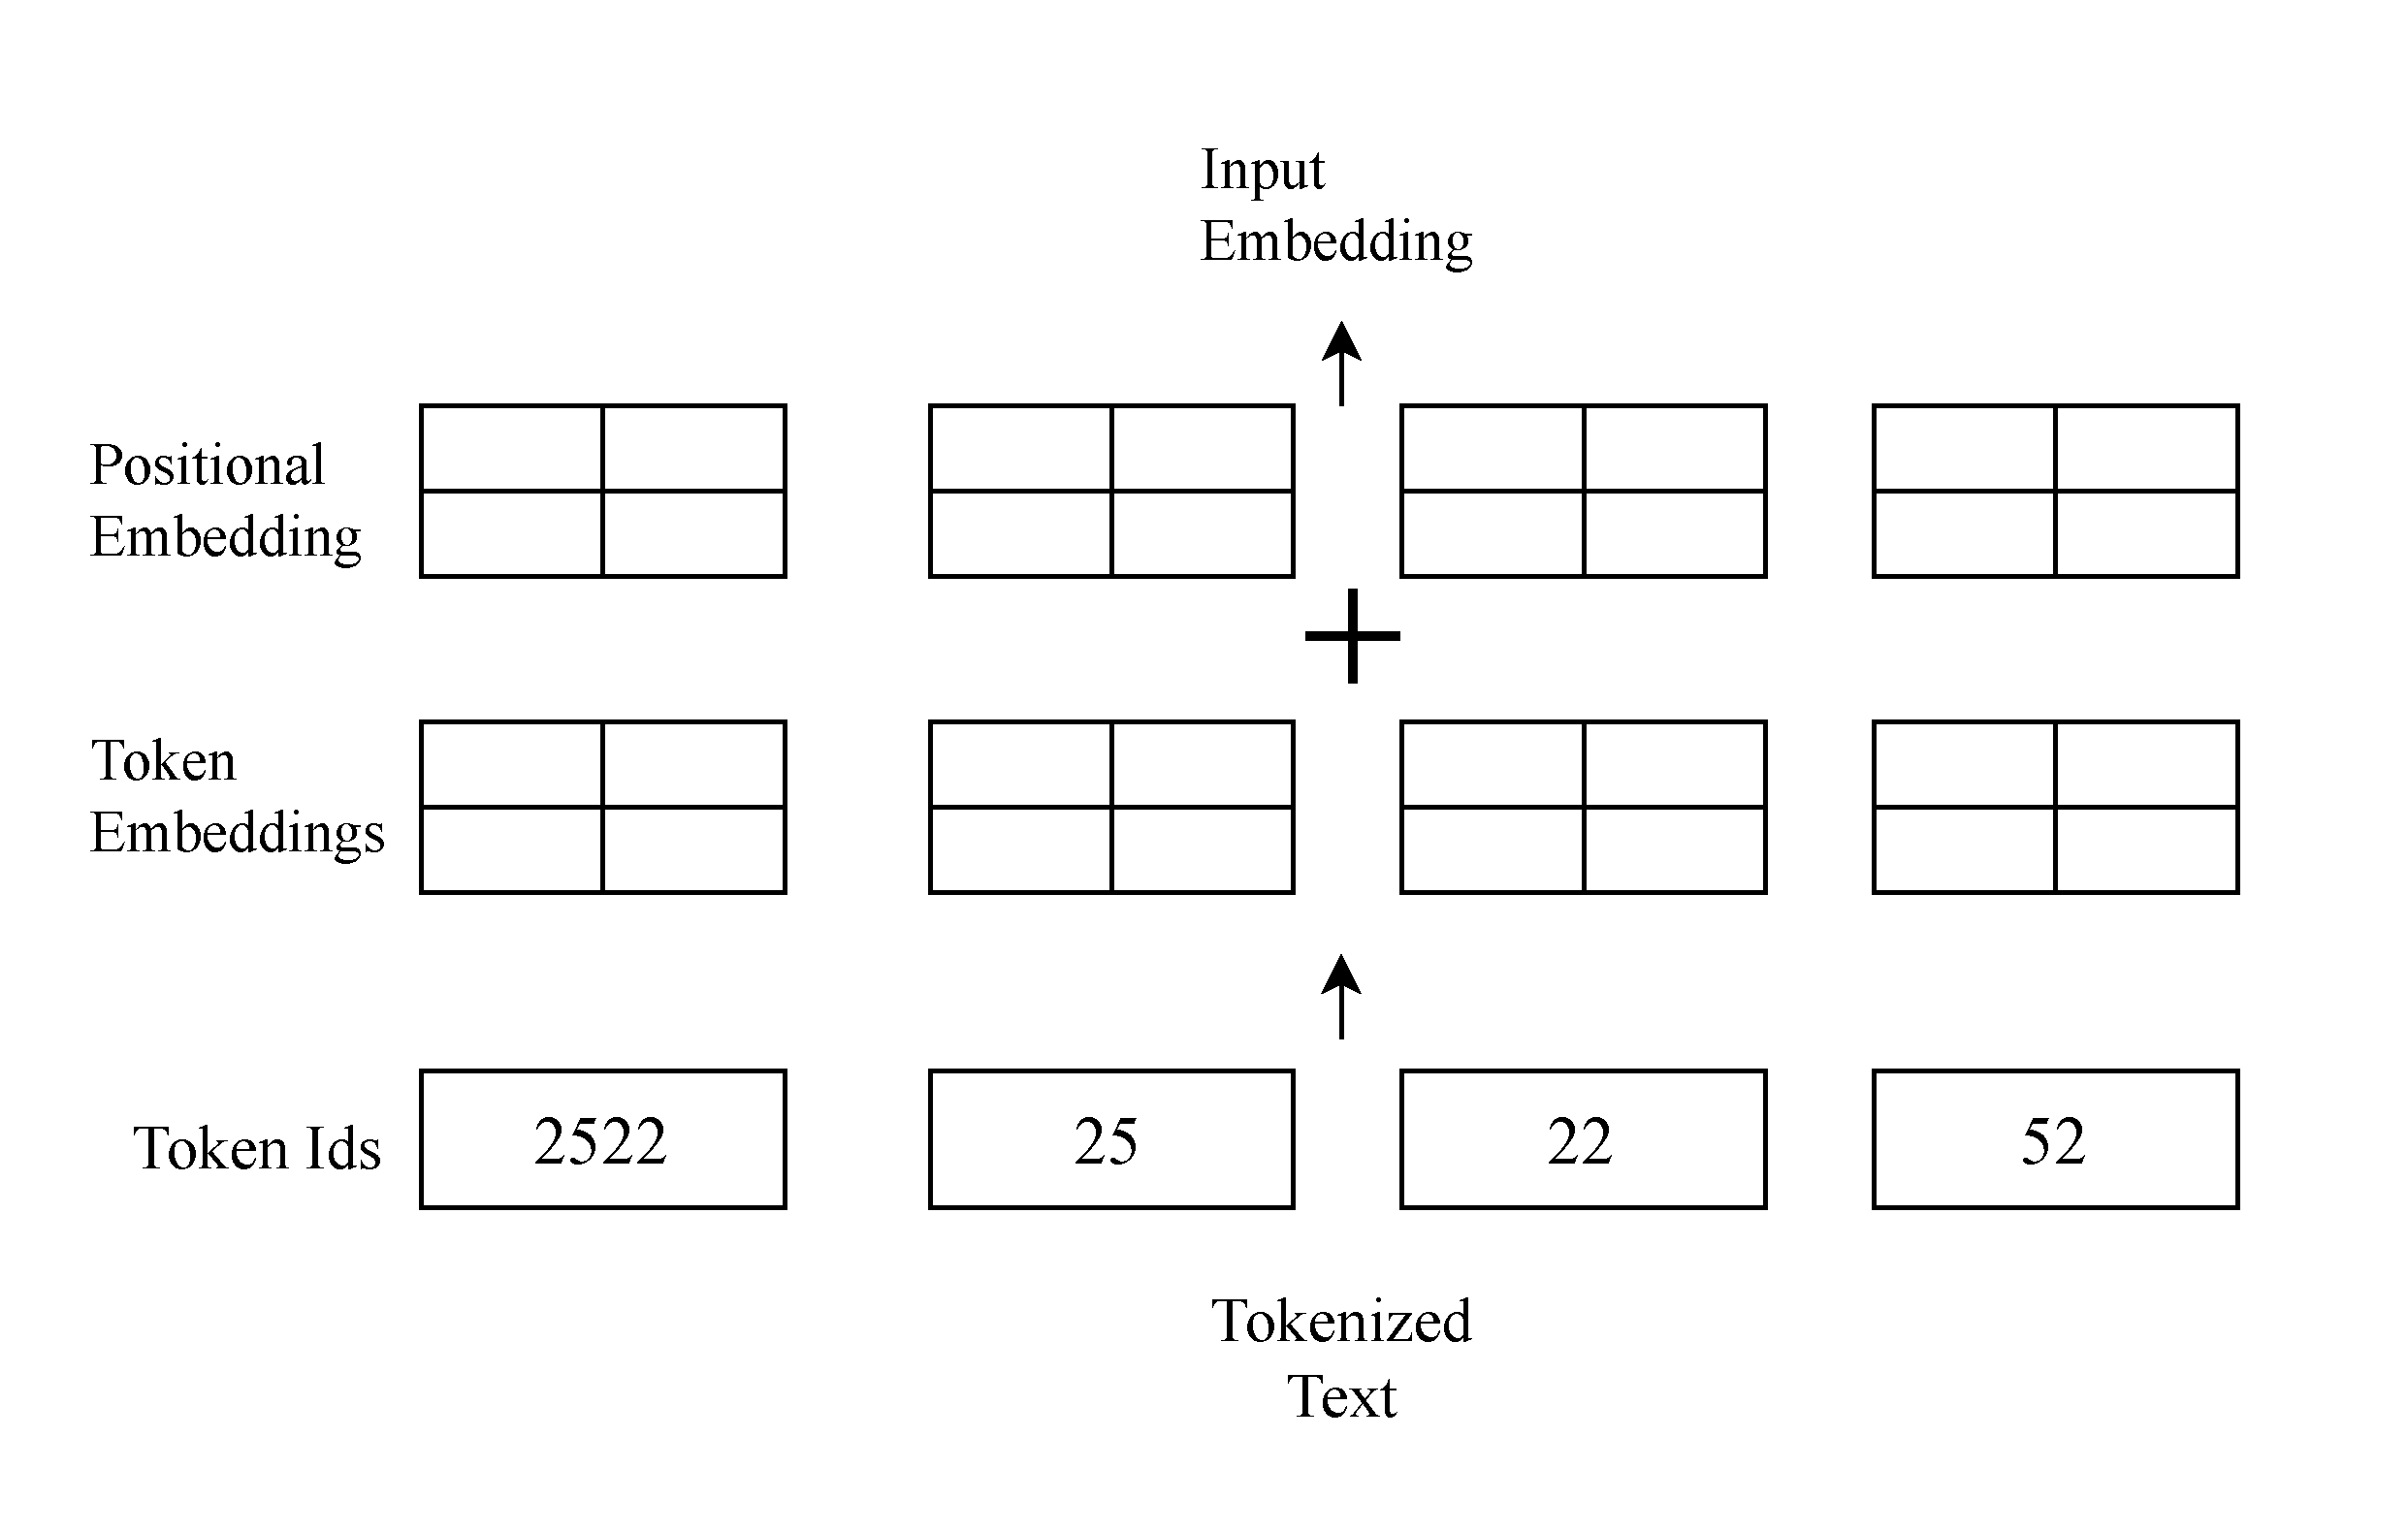
\includegraphics[width=\linewidth]{Images/SLM/Implementation Details/Embedding.pdf}%
    }{%
        \fbox{\parbox{0.92\linewidth}{\centering
        Embedding illustration file not available in the repository.\\
        This figure is intended to show token embeddings combined with positional embeddings before being passed into the decoder.}}%
    }
    \caption{Token and Positional Embedding}
\end{figure}

\subsubsection{Masked Multi-Head Attention Mechanism}
The Multi-Head Attention module uses a casual scaled dot product attention mechanism with multiple heads to create a context vector. 

\begin{figure}[H]
    \centering
    \IfFileExists{Images/SLM/Implementation Details/AttentionMechanism.pdf}{%
        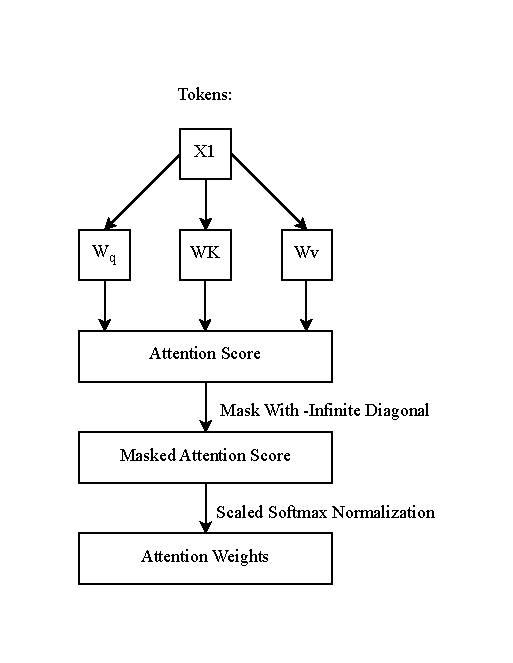
\includegraphics[width=1\linewidth]{Images/SLM/Implementation Details/AttentionMechanism.pdf}%
    }{%
        \fbox{\parbox{0.92\linewidth}{\centering
        Attention mechanism illustration file not available in the repository.\\
        This figure is intended to summarize causal masked multi-head attention with query, key, and value projections.}}%
    }
    \caption{Attention Mechanism}
    \label{fig:Attention Mechanism}
\end{figure}

\begin{itemize}
    \item \textbf{Initialization and projection: }
    The input tensor has shape $(B, T, d_{in})$ where $B$ is the batch size and $T$ is the sequence length. The output dimension $d_{out}$ should be divisible by the number of heads $h$, i.e.,
    $
      d_k = \frac{d_{out}}{h}
    $
    The first three linear layers $W_{\text{query}}, W_{\text{key}}, W_{\text{value}}$ are initialized to project input embeddings into query, key, and value vectors. A causal mask using an upper triangular matrix is applied, ensuring that during training the model attends only to previous positions, preventing information leakage.

    $$Q = XW_Q \quad K = XW_K \quad V = XW_V$$

    The data is projected once and reshaping of resulting tensors is done instead of using separate layers for each head.
    
    \item \textbf{Scaled dot-product attention: }
    First the raw attention scores are calculated by performing matrix multiplication between queries and the transposed keys. To prevent information leakage a casual mask M an upper triangular matrix of negative infinity is used with scores. Then the attention weights are computed by scaling the scores by $\sqrt{d_k}$ and applying a Softmax function:

    \begin{equation}
        \text{Attention}(Q, K, V) = \mathrm{softmax}\!\left(\frac{QK^{T}}{d_k} + M\right)V
    \end{equation}
    The scaling factor $\sqrt{d_k}$ is critical here to counteract the effect of large dot products pushing the Softmax function into regions with extremely small gradients.

    After applying the attention weights to the value vectors V, the resulting context vectors from all h heads are transposed and concatenated to restore the original sequence shape (B,T,$d_{out}$). Finally, a linear output projection W is applied to mix the concatenated representations across heads, yielding the final output of the module.
    
\end{itemize}

\subsubsection{Model Creation}
\textbf{Layer Normalization and GELU activation}\\
For layer normalization which normalizes activations across the embedding dimension for each token independently to compute the mean and variance along the last dimension.

\begin{equation}
\hat{x} = \frac{x - \mu}{\sqrt{\sigma^2 + \epsilon}}, \quad
y = \gamma \hat{x} + \beta
\end{equation}


\begin{table}[ht]
\caption{Model Hyperparameters}
\centering
\begin{tabular}{|l|l|}
\hline
\textbf{Parameter} & \textbf{Value} \\
\hline
Vocabulary Size ($vocab\_size$) & 50257 \\
Context Length ($context\_length$) & 1024 \\
Dropout Rate ($drop\_rate$) & 0.0 \\
QKV Bias ($qkv\_bias$) & True \\
Embedding Dimension ($emb\_dim$) & 768 \\
Number of Layers ($n\_layers$) & 12 \\
Number of Heads ($n\_heads$) & 12 \\
\hline
\end{tabular}
\end{table}

This feed network uses the Gaussian Error Linear Unit (GELU) activation. It introduces non-linearity while allowing small negative values to pass smoothly.

\begin{equation}
\mathrm{GELU}(x) = 0.5 \, x \left[ 1 + \tanh \left( \sqrt{\frac{2}{\pi}} \left( x + 0.044715 \, x^3 \right) \right) \right]
\end{equation}

\textbf{Transformer block and model}\\
The first input goes through layer normalization. The feed forward part consists of two linear layers. The first expands the embedding dimension to 4 times its size, applies GELU and projects the original embedding dimension towards the second linear layer. Which is followed by multi-head attention sub-layer. A dropout is applied to the attention output and a residual connection adds a shortcut. This process is repeated multiple times to form a core transformer stack. The model begins with a token embedding layer and positional embedding of the same dimensions. Which then flows to the stack of n\_layers of the transformer block. A last layer normalization is applied and linear output head is used that projects the embeddings to a vocabulary size. The result logits represents unnormalized probabilities over next token for each position in the sequence.

\subsection{RAG}

\subsubsection{Scraping}

The data collection layer maintains the knowledge base with the latest news articles from Nepali-based English news outlets. The pipeline uses RSS feeds as opposed to scraping raw HTML, which is inconsistent and frequently changed. It does not perform any HTML parsing except where no RSS feed is available.

\textbf{RSS Feeds}

RSS feeds are XML files published by news sites for automated consumption. Feed items consist of an article URL, title, time of publication, and an optional short description. Since all sites share the same format, a large number of sources can be processed by a single parser. \texttt{feedparser} is used to download and process all feeds in the pipeline. The scraper, on a per-entry basis, extracts the URL and date, verifies the entry has not already been processed, and queues it for full-text extraction. Eighteen feeds are registered across major English-language Nepali news sources including \textit{Kathmandu Post}, \textit{Online Khabar}, \textit{Spotlight Nepal}, \textit{My Republica}, \textit{The Himalayan Times}, and \textit{Nepal News}.

\textbf{Article Extraction}

For every URL, \texttt{newspaper4k} downloads the page and applies heuristics to locate the main article text. It strips away navigation menus, sidebars, advertisements, and footer material, delivering clean prose. This approach works effectively across most sites and requires no site-specific configuration.

Some websites block \texttt{newspaper4k}'s default requests. In such cases the pipeline falls back to a manual process. It issues an HTTP GET request with a browser-like \texttt{User-Agent} via the \texttt{requests} library and parses the HTML using \texttt{BeautifulSoup4}. Paragraph tags within the main content area are extracted, their text is merged, and the article body is reconstructed. This fallback is applied only to sites known to block automated scrapers.

\textbf{Quality Filtering and Deduplication}

Two checks are performed before any article enters the pipeline. First, the URL is checked against an SQLite database; if already present, the article is skipped entirely, preventing duplication across repeated runs. Second, articles containing fewer than 80 words of extracted text are discarded, as short extractions typically indicate a failed parse, a paywall stub, or an advertisement fragment. A delay of 1.0 second is enforced between requests to maintain low server load.

\begin{table}[H]
\caption{Scraping Configuration}
\label{tab:scraping_config}
\centering
\begin{tabularx}{\linewidth}{|l|l|X|}
\hline
\textbf{Parameter} & \textbf{Value} & \textbf{Purpose} \\
\hline
Number of RSS feeds & 18 & Coverage across major English outlets \\
Max articles per feed & 100 & Upper ceiling per refresh cycle \\
Minimum word count & 80 & Filters failed extractions \\
Request delay & 1.0 s & Polite crawling \\
Request timeout & 15 s & Handles slow archival pages \\
Primary extractor & \texttt{newspaper4k} & Clean article body extraction \\
Fallback extractor & \texttt{requests} + \texttt{BeautifulSoup4} & Blocked-site handling \\
\hline
\end{tabularx}
\end{table}

\subsubsection{Indexing}

Indexing converts unstructured articles into a structured, searchable format allowing the system to locate appropriate content quickly. In the absence of indexing, query processing would search every document, which is not realistic when dealing with large collections. The system uses dense vector indexing, where documents and queries are represented in the same continuous space such that similar documents are geometrically close. This approach is stronger compared to previous inverted-index approaches such as BM25, which rely on word overlap and fail when the wording changes.

\textbf{FAISS IndexFlatIP}

The index is built on FAISS IndexFlatIP, where Flat denotes exhaustive exact search and IP denotes inner product as the similarity metric. Given a query vector $\mathbf{q} \in \mathbb{R}^{384}$ and $N$ stored chunk vectors, the index computes:

\begin{equation}
    s(\mathbf{q}, \mathbf{d}_i) = \mathbf{q} \cdot \mathbf{d}_i
\end{equation}

All vectors are L2-normalised prior to storage ($\|\mathbf{q}\| = \|\mathbf{d}_i\| = 1$), so the inner product of two vectors equals their cosine similarity, scoring 1.0 for identical semantic direction. IndexFlatIP was chosen over approximate alternatives such as IndexIVFFlat and IndexHNSWFlat because at this scale, exact search completes in milliseconds on CPU. Parameters for IndexIVFFlat are retained in configuration for when the dataset scales to millions of chunks.

\textbf{Chunking}

The embedding model all-MiniLM-L6-v2 has a maximum sequence length of 256 word-pieces, while most articles run to 800--1500 words. Encoding an entire article as a single vector produces an averaged representation of all its content, meaning a query targeting a specific passage would not match well. Articles are instead divided into overlapping segments along sentence boundaries. Sentences are first extracted using NLTK's Punkt tokeniser, then greedily accumulated into a buffer until the estimated token count reaches 500 tokens, approximated as:

\begin{equation}
    \hat{t} = \frac{w}{0.75}
\end{equation}

where $w$ is word count and the divisor accounts for the average English subword tokenisation ratio of approximately 1.33 tokens per word. When the buffer fills, it is finalised as a chunk and a new buffer is seeded with the last 50 tokens of sentences from the previous chunk. This overlap ensures that any passage crossing a chunk boundary is fully represented in at least one chunk, preventing retrieval failure on boundary-spanning content. Each chunk inherits the parent article's metadata --- title, URL, publication date, and source --- for downstream citation.

\textbf{Embedding and Storing}

Each chunk is encoded by passing it through all-MiniLM-L6-v2, which applies six transformer layers of multi-head self-attention and mean-pools the final hidden states across all token positions constraining it to the unit hypersphere and enabling cosine similarity via inner product as required by FAISS IndexFlatIP. 

\begin{equation}
    \mathbf{e} = \frac{1}{T} \sum_{t=1}^{T} \mathbf{h}_t^{(L)}
\end{equation}

producing a 384-dimensional vector $\mathbf{e}$. This vector is then L2-normalised:

\begin{equation}
    \hat{\mathbf{e}} = \frac{\mathbf{e}}{\|\mathbf{e}\|_2}
\end{equation}


\subsubsection{Retrieval}

The retriever encodes the query string with the all-MiniLM-L6-v2 model, which corresponds to the same embedding pipeline as the indexing one, and then the query is matched with a set of retrieved results. The 384-dimensional resultant is L2-normalised. This vector is then submitted to a FAISS IndexFlatIP index where the inner product is computed with each of the stored chunk vectors. Since all the vectors are unit normalised, the inner product is the similarity of cosines. The highest-ranked candidates are returned in terms of the similarity score.

\textbf{Cosine Similarity}

Cosine similarity compares the angle between two high-dimensional vectors that give a semantic similarity no matter how intense it is. It is computed as the dot product of the vectors divided by the product of the magnitudes of the vectors. For a query vector $\mathbf{q}$ and a chunk vector $\mathbf{d}$, it is defined as:

\begin{equation}
    \cos(\theta) = \frac{\mathbf{q} \cdot \mathbf{d}}{\|\mathbf{q}\| \|\mathbf{d}\|}
\end{equation}

Given that all vectors are normalised, the magnitude is 1.0, hence the score is simply the inner product with values between 0.0 and 1.0. A rating of 1.0 reflects complete alignment; the closer the score to 0.0, the more orthogonality. Any chunk with a score below 0.45 is dropped prior to processing, and a hard relevance floor is used to eliminate weakly relevant content.

\textbf{Time-Decay Scoring}

Raw cosine similarity does not take time into consideration. An article that is two years old may be quite relevant but will not be as useful as a moderately similar one that was published yesterday. To address this, each candidate is assigned a time-decay factor depending on the number of days that the parent article is old:

\begin{equation}
    s_{\text{decay}} = e^{-\lambda d}
\end{equation}

where $d$ is the article age in days and the decay rate $\lambda$ is set to 0.02. This results in a gradual depreciation of articles older than 2 or 3 years while retaining a significant freshness score, eliminating unnecessary partiality to older content when giving preference to more recent ones.

\textbf{Blended Score}

The cosine similarity score and the time-decay score are combined into a single blended ranking score:

\begin{equation}
    s_{\text{final}} = 0.7 \cdot s_{\text{cosine}} + 0.3 \cdot s_{\text{decay}}
\end{equation}

The weight of semantic similarity is 70\% and freshness is 30\%. This combination maintains topical relevance as the primary cue but applies freshness as a tiebreaker should there exist a close call in scores. This blended score is used to rank the candidates with the five highest selected moving to reranking. A hard filter of 730 days is also applied; any chunk older than that is excluded regardless of similarity.

\textbf{CrossEncoder Reranking}

The original FAISS output is based on a bi-encoder which encodes query and chunk independently, producing coarse-grained relevance. In order to refine this ranking, the CrossEncoder model \texttt{cross-encoder/ms-marco-MiniLM-L-6-v2} reevaluates every candidate. In this model the query and chunk are concatenated into a single input and jointly encoded, such that token-level interactions can occur that the bi-encoder is unable to capture. It generates a scalar relevance score for each pair and the candidates are re-ranked. The top-K chunks with the best scores after this step are sent to the generation component.

\subsubsection{Augmentation}

Reranking is followed by a combination of the final list of pertinent chunks and the initial user query to create a structured prompt. The prompt places the chunks above the question, instructing the language model to use the presented context to formulate its response instead of drawing on its own knowledge. This step is necessary as the model otherwise generates answers from its frozen training data, which may be outdated or hallucinated. The system maintains factually grounded responses by pre-loading verified, source-attributed content.

Since the context window of the language model is constrained, every chunk is truncated to 1200 characters so that the entire prompt including the query fits within the input limit of the custom small model. The final prompt is then passed to the generator with a temperature of 0.1 and greedy decoding, producing deterministic output that is closely related to the material provided.

\subsubsection{Generation}

The augmented prompt is provided to a small language model that is custom fine-tuned and generates the response. The prompt includes the retrieved context chunks and the query created by the user, and the model provides a response based solely on that context. It is beneficial to use a domain-specific model rather than a general model to maintain the tone and style of Nepali news content and not to be distracted by irrelevant information.

\textbf{Tunable Parameters and Their Effect}

The retrieval stage exposes several parameters that directly control the quality and coverage of what the generator receives as context. Their adjustment consists of trade-offs rather than universally correct values.

The minimum cosine similarity threshold governs the strictness of the relevance floor. Setting it high will include only chunks that are close matches to the query, which enhances precision but exposes it to the chances of eliminating relevant material that has been phrased differently. When the threshold is excessive, the generator may refuse to respond or respond half-heartedly. Reducing the threshold increases the size of the pool, which boosts recall and decreases refusals, but also adds loosely related chunks that introduce noise and draw the response away from the correct information.

The top-K parameter decides the number of chunks assembled into the final generation context. A higher top-K gives broader coverage, which is useful when a query requires synthesising information from multiple sources. Nevertheless, a larger top-K also increases the likelihood of incorporating marginally relevant or contradictory chunks, resulting in inconsistent or unfocused answers. A smaller top-K keeps the context tight and focused, producing sharper answers to narrow factual questions but potentially missing supporting evidence for questions that demand wider context.

The decay rate controls how aggressively older articles are down-weighted during retrieval. A high decay rate causes freshness scores to decline quickly with age, meaning the generator tends to receive recent content almost always, even when older articles are more semantically relevant. This is appropriate when recency is critical but harmful when the topic benefits from older authoritative sources. A lower decay rate flattens the freshness curve, allowing older articles to compete on semantic relevance alone. This improves coverage for historical or slowly evolving topics but may occasionally surface outdated information on time-sensitive queries.

The semantic weight and freshness weight together determine the balance between these two signals in the final ranking score. Increasing semantic weight biases the ranking toward topical relevance, making the system behave closer to a pure vector similarity search. Increasing freshness weight shifts the ranking toward recency, such that the generator may receive very recent articles even when they are only loosely related to the query. Adjusting these two weights is the primary mechanism for tuning the relevance and timeliness balance of the context delivered to the generator.
\newpage
\section{\MakeUppercase{Result and Analysis}}
	
\subsection{ASR}
\subsubsection{Word Error Rate (WER) Comparison and Analysis in FastConformer}
\begin{figure}[H]
	\centering
	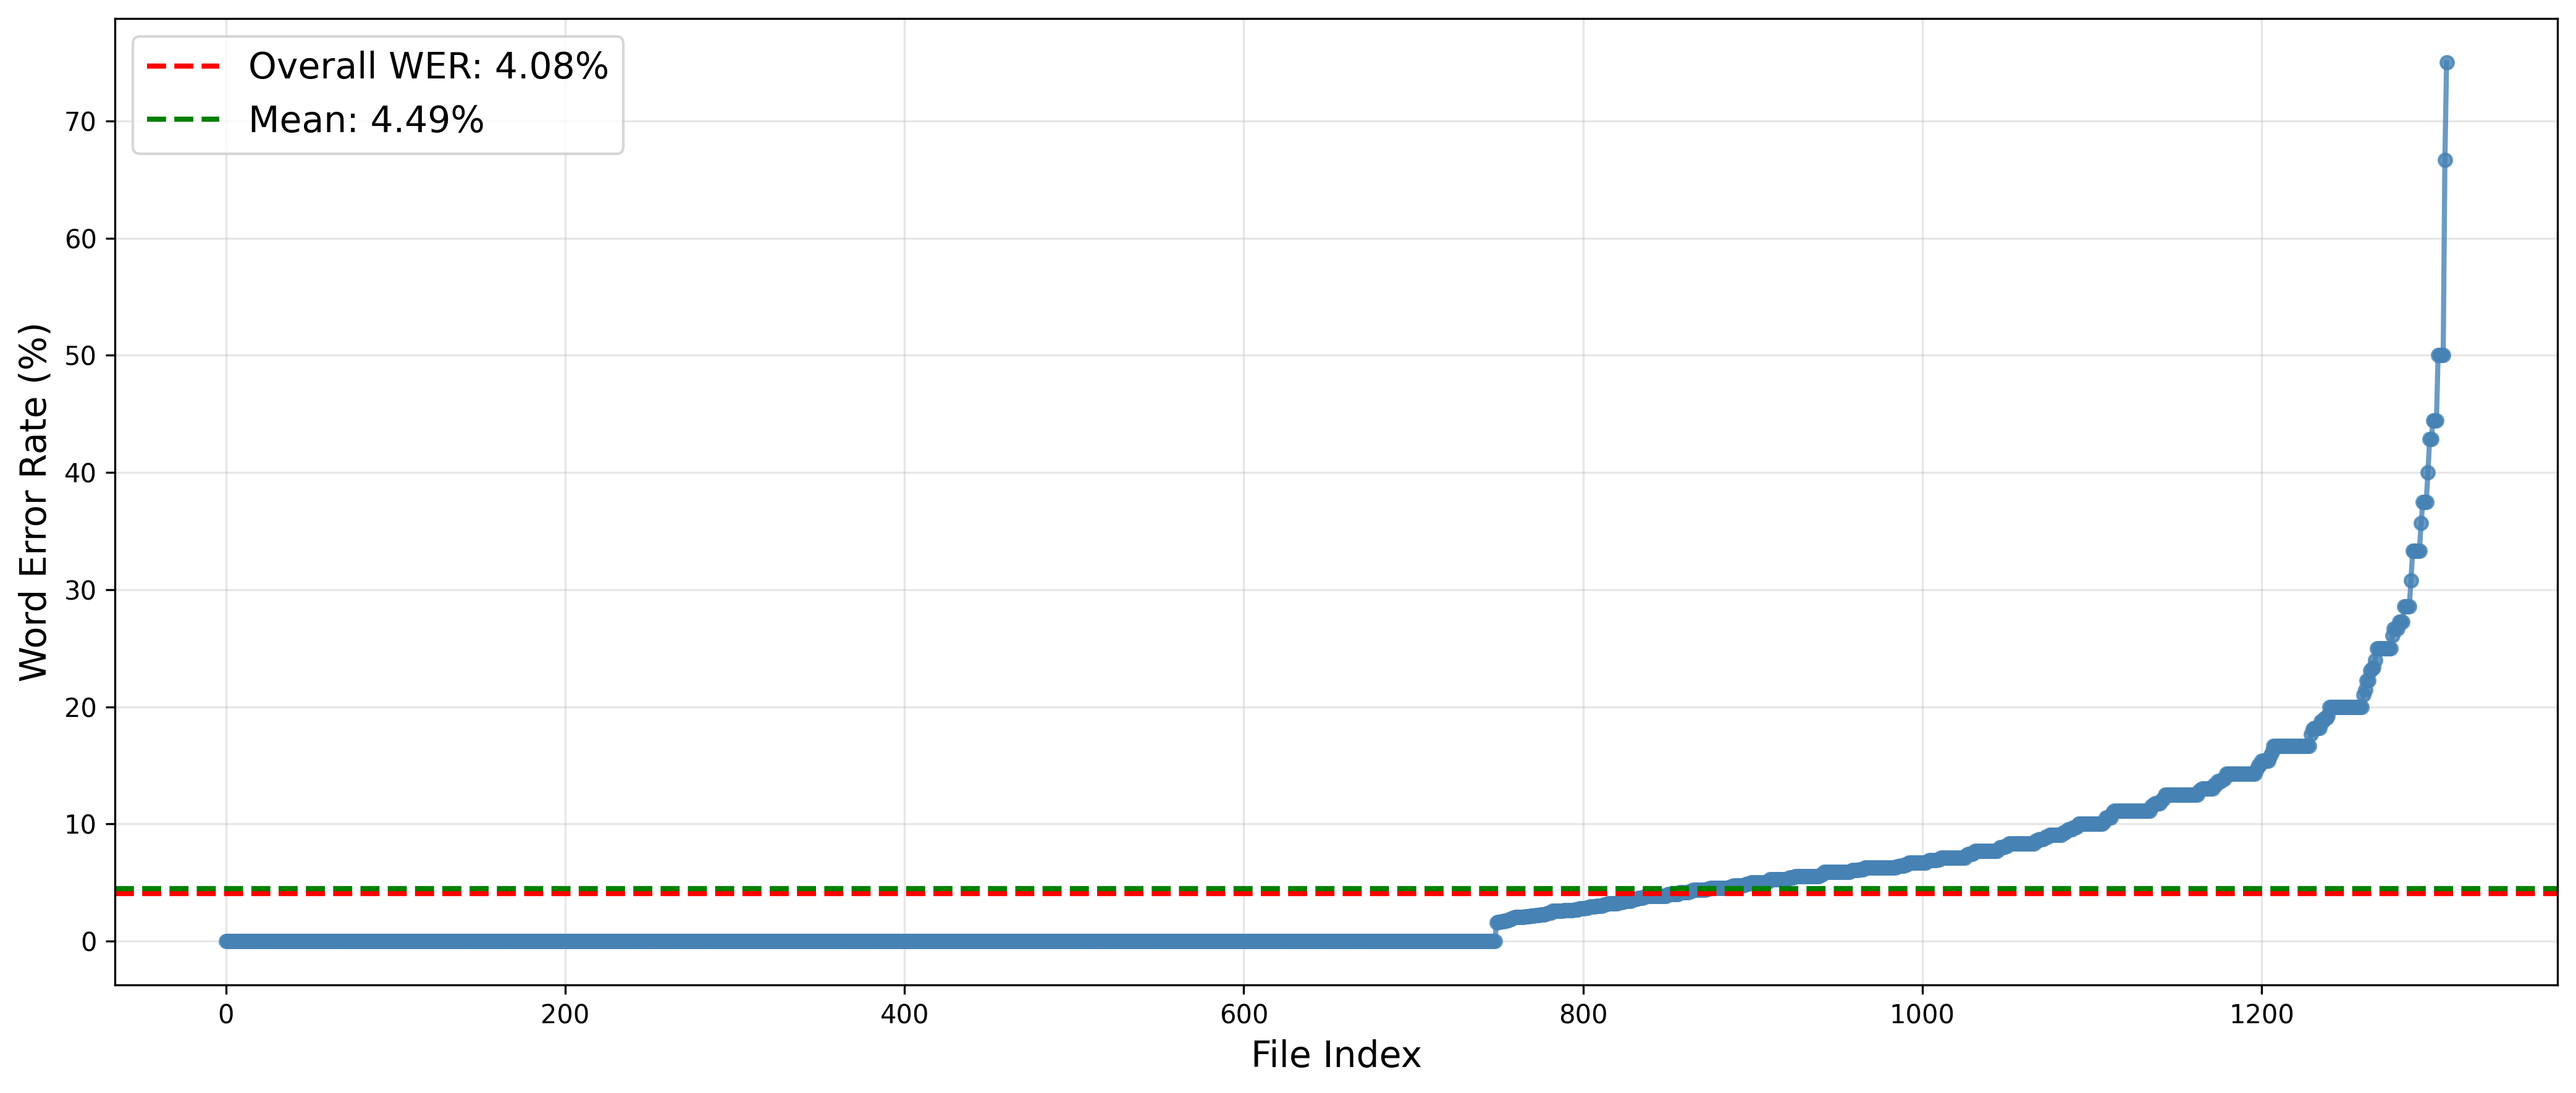
\includegraphics[width=\linewidth]{Images/ASR/Results/shaswot-graphs/WER_LibriSpeech.png}
	\caption{WER on LibriSpeech}
\end{figure}

\begin{table}[H]
	\centering
	\begin{tabular}{|l|c|c|}
		\hline
		\textbf{Model} & \textbf{WER} & \textbf{Parameters} \\
		\hline
		Deep Speech 2 & 5.33 & 110M \\
		Gated ConvNets & 4.8 & 100M \\
		Seq-to-Seq Attention (LSTM Based) & 3.82 & 50M--100M \\
		Convolution Speech Recognition & 3.26 & 30M--70M \\
		wav2vec-wav2letter & 2.7 & 30M / 50M \\
		Transformer & 2.6 & 60M--100M \\
		Squeezeformer (L) & 2.47 & 50M \\
		LSTM Transducer & 2.23 & 40M--80M \\
		Conformer (M) & 2.0 & 50M \\
		Stateformer & 1.76 & 40M--60M \\
		\textbf{Fast Conformer} & \textbf{6.14} & \textbf{13.2M} \\
		\hline
	\end{tabular}
	\caption{Word Error Rate (WER) and parameter count of models trained on the LibriSpeech dataset}
	\label{tab:wer_librispeech_models}
\end{table}
The fine-tuned model has only 13.2 million parameters, which is about 4x to 8x times fewer than smaller architectures (e.g., Conformer-M, ~50 million parameters) and larger ones (e.g., DeepSpeech 2, ~110 million parameters). This compactness makes the architecture very compatible with edge devices and low-latency applications. The encoder is 98.6\% of the total number of parameters, meaning that it washes up all the model capacity, the decoder is insignificant, consisting of only 181K  parameters. This distribution is consistent with CTC based structures that avoid the use of complicated auto-regressive decoders, which limit both memory size and inference complexity.

The achieved WER of 6.14\% per cent is higher than the performance of higher-ranking models, most of which use three to eight times the number of parameters and large amounts of data augmentation, nevertheless, it is a strong performance-per-parameter trade-off. In the case of a situation where constraints in model size, power consumption, or real-time response are involved, the existing model provides a realistically compromised state. The use of a CTC-BPE hybrid output scheme avoids the use of outside language models during decoding, which simplifying the scheme, rather than the many transducer or attention-based models, retains a reasonable degree of sub-word level generalization.

The WER of the model can be further improved to 4.08\% when using greedy decoding, a relatively inexpensive method of choosing the most likely token at each iteration without using a beam search or outside language model rescoring. The only difference is that this can be seen in the red dashed line (Overall WER: 4.08\%), much lower than the green dashed line that shows the average WER (4.49\%), across utterances, shows that not only does greedy decoding increase average accuracy, but also makes performance less varied. This finding highlights the strength of the CTC-BPE hybrid output layer: it is simple with limited decoder footprint, but it produces highly competitive transcription quality, particularly when the factors of inference constraints are important and marginal gains in complex modes of decoding are traded in at the cost of latency and compute efficiency.

\subsubsection{WER, CER and Size Analysis of IndicConformer}
 
\begin{table}[H]
\centering
\begin{tabular}{|l|r|r|}
\hline
\textbf{Model} & \textbf{Parameters} & \textbf{WER (\%)} \\
\hline
Whisper Tiny & 39M & 101.8 \\
Whisper Base & 74M & 102.4 \\
Whisper Small & 244M & 69.5 \\
Whisper Medium & 769M & 54.4 \\
IndicConformer finetuned & 129M & 31.40 \\
\hline
\end{tabular}
\caption{WER (\%) on Clean Fleurs Test Set}
\label{tab:clean_wer}
\end{table}
The clean Fleurs test set results demonstrate that there is a clear comparison of the various Whisper models and the fine-tuned IndicConformer model. Although the models of Whisper get better as they get larger, as Whisper Tiny and Base have very bad WER of 100 and above and 69.5 and 54.4 percent, they are still 10 times worse than the model of IndicConformer that was finetuned. Although it has less parameters (129M), the fine-tuned IndicConformer shows a much lower WER of 31.40\%. This comparison indicates that the IndicConformer fine-tuned model is more effective than all variants of Whisper, which emphasizes that fine-tuning and architecture design play a greater role in the model rather than adding more size to it.

\begin{table}[H]
\centering
\footnotesize
\setlength{\tabcolsep}{5pt}
\begin{tabular}{|l|l|c|c|c|c|c|}
\hline
\rule{0pt}{3ex}\textbf{Model} & \textbf{Type} & \textbf{Size} & \textbf{CER} & \textbf{WER} & \textbf{\shortstack{Global \\[2pt] CER}} & \textbf{\shortstack{Global \\[2pt] WER}} \\
\hline
IndicConformer & NeMo (original) & 493.05 & 15.03 & 35.59 & 13.35 & 33.88 \\
IndicConformer & NeMo (finetuned) & 493.05 & 14.24 & 33.75 & 13.27 & 32.55 \\
IndicConformer & ONNX (full) & 470.22 & 14.24 & 33.75 & 13.88 & 32.49 \\
IndicConformer & ONNX (quantized) & 133.94 & 16.08 & 37.96 & 15.01 & 36.77 \\
\hline
\end{tabular}
\caption{Accuracy Metrics on Noisy Fleurs Test Set}
\label{tab:noisy_accuracy}
\end{table}

The table compares the performance in noisy environments, which gives the character error rate (CER) and word error rate (WER) and global measures. The original NeMo IndicConformer has a CER of 15.03\% and WER of 35.59\%. Once finetuned, the model becomes significantly better: CER declines to 14.24\% and WER declines to 33.75, indicating that finetuning is not only helpful in improving clean speech, but also enhances noise resistance. The trend of global measures is similar, as global CER has decreased to 13.27\% and global WER to 33.55\%, which means that all measures gain continuously throughout the whole data range.

The ONNX full model has the same CER and WER as the finetuned NeMo model with a slight reduction of the model size to 470.22 MB. The ONNX quantized model which is optimized to run at 133.94 MB only, experiences a slight degradation: CER increases to 16.08\% and WER to 37.96\%, with global CER/WER also on the rise, a classic trade-off between model size and accuracy.

\subsubsection{Qualitative Analysis}
To illustrate examples of model predictions on held-out utterances, below there are three representative samples, each paired with its ground-truth reference, the model’s hypothesis, and the corresponding Word Error Rate (WER):

These examples demonstrate that the model accurately captures most of the semantic content. Errors are primarily lexical (e.g., “latter” vs. “latter day”, “to day” vs. “today”) or morphological, which are common in CTC-based systems without external language models. Notably, the model achieves perfect transcription on complex formal language in the second example, highlighting its robustness on well-articulated speech

\subsubsection{Training Dynamics}
\begin{figure}[H]
	\centering
	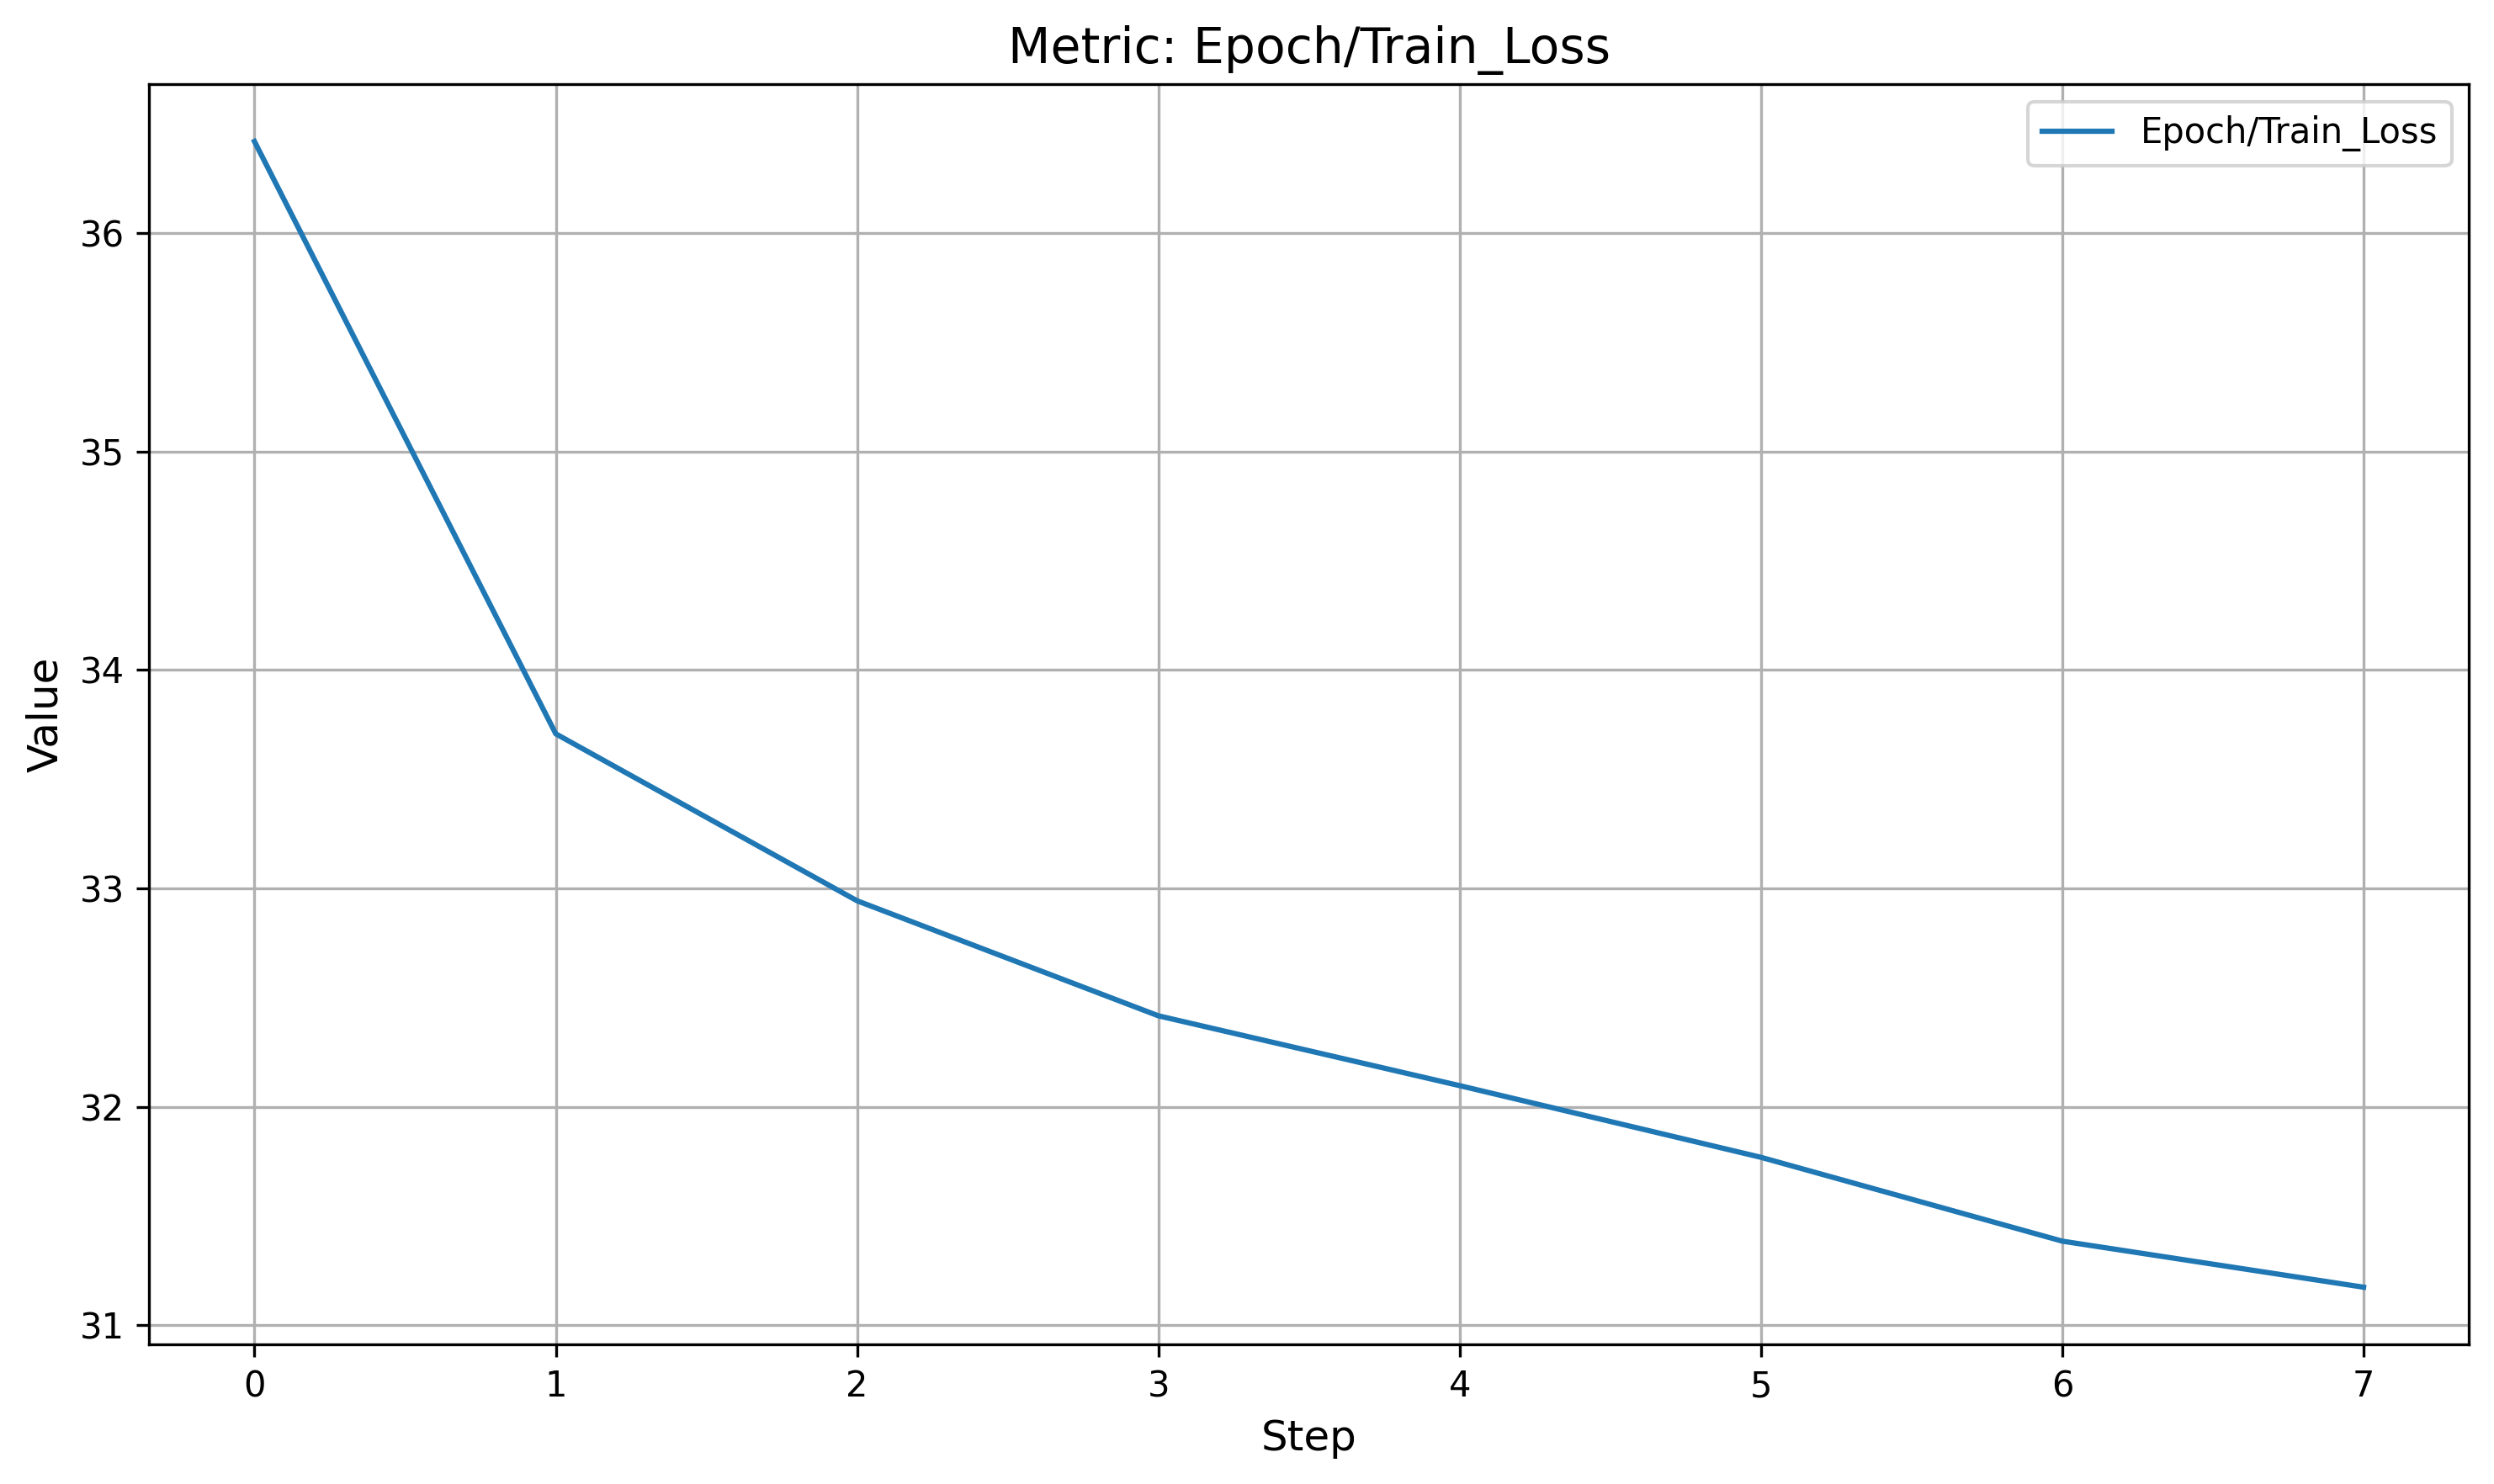
\includegraphics[width=\linewidth]{Images/ASR/Results/shaswot-graphs/EpochTrain_Loss.png}
	\caption{Epoch-wise Training Loss}
\end{figure}

Training Loss (Figure 6-1) decreases steadily from 36.2 to 31.2, indicating consistent learning.

\begin{figure}[H]
	\centering
	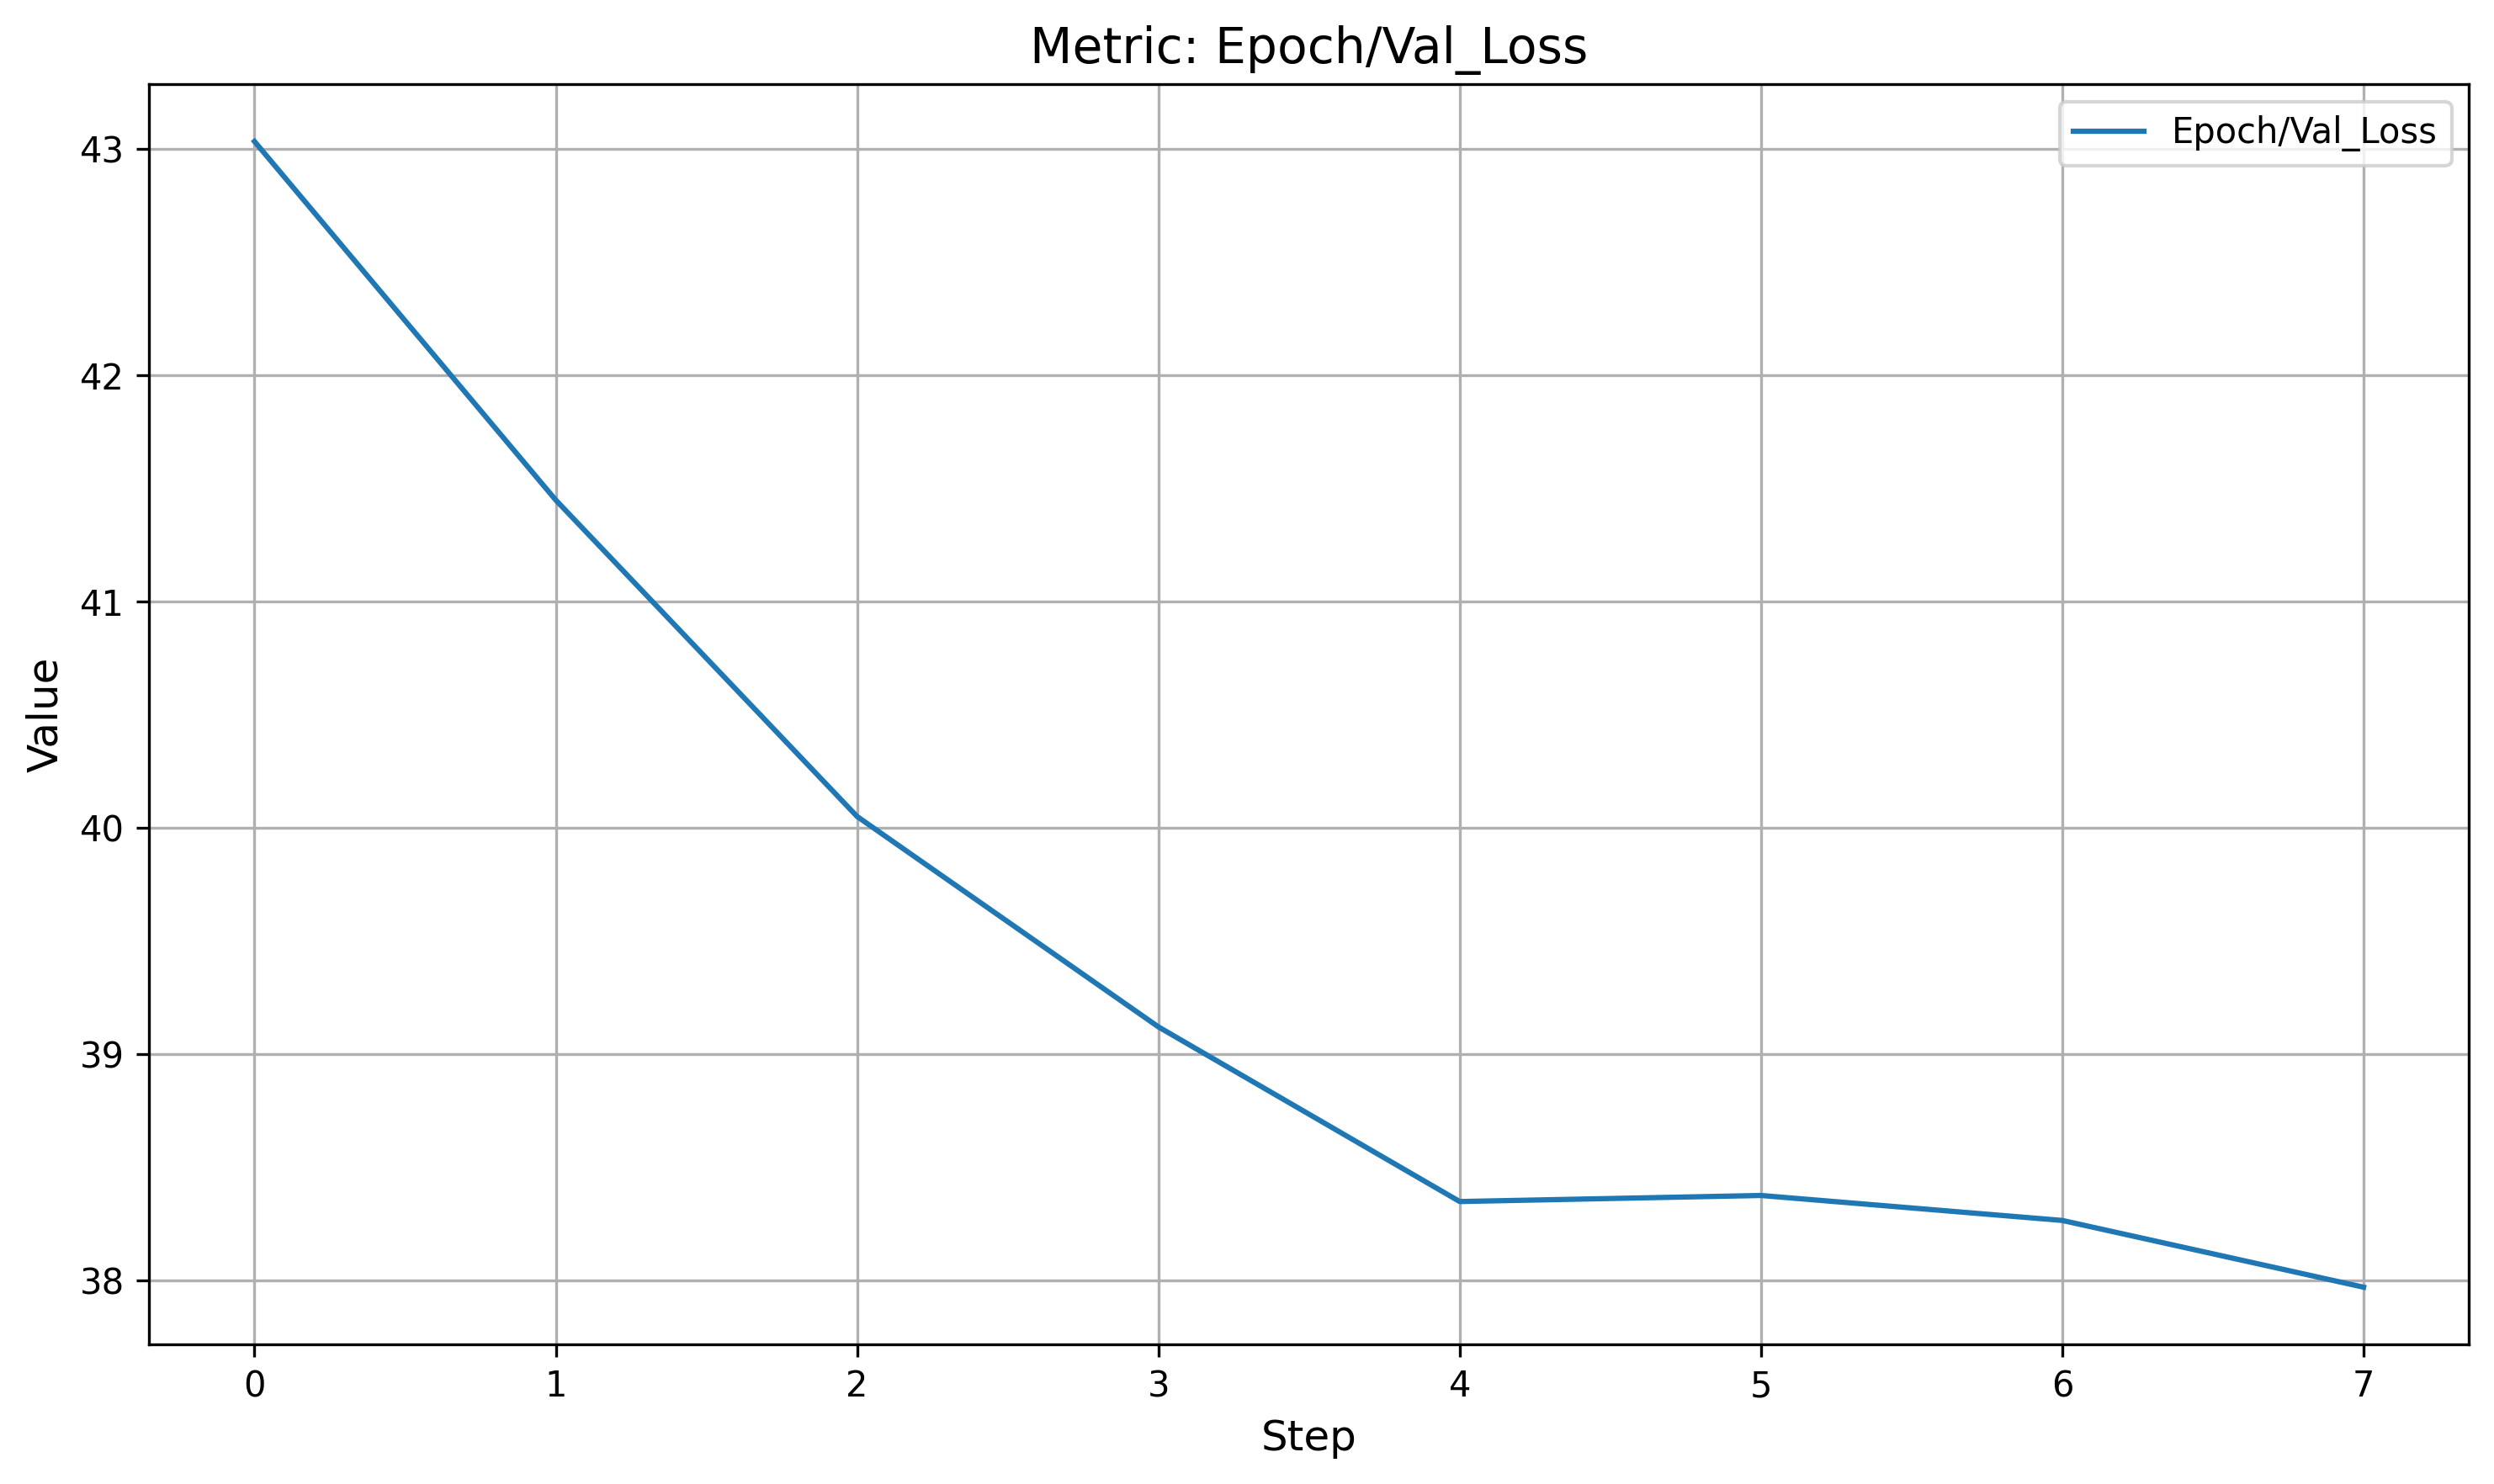
\includegraphics[width=\linewidth]{Images/ASR/Results/shaswot-graphs/EpochVal_Loss.png}
	\caption{Epoch Wise Validation Loss}
\end{figure}
Validation Loss (Figure 6-2) shows a similar downward trend, reaching 37.9 at epoch 7, with only minor fluctuations (e.g., a small uptick at epoch 5), suggesting good generalization without severe overfitting.

\begin{figure}[H]
	\centering
	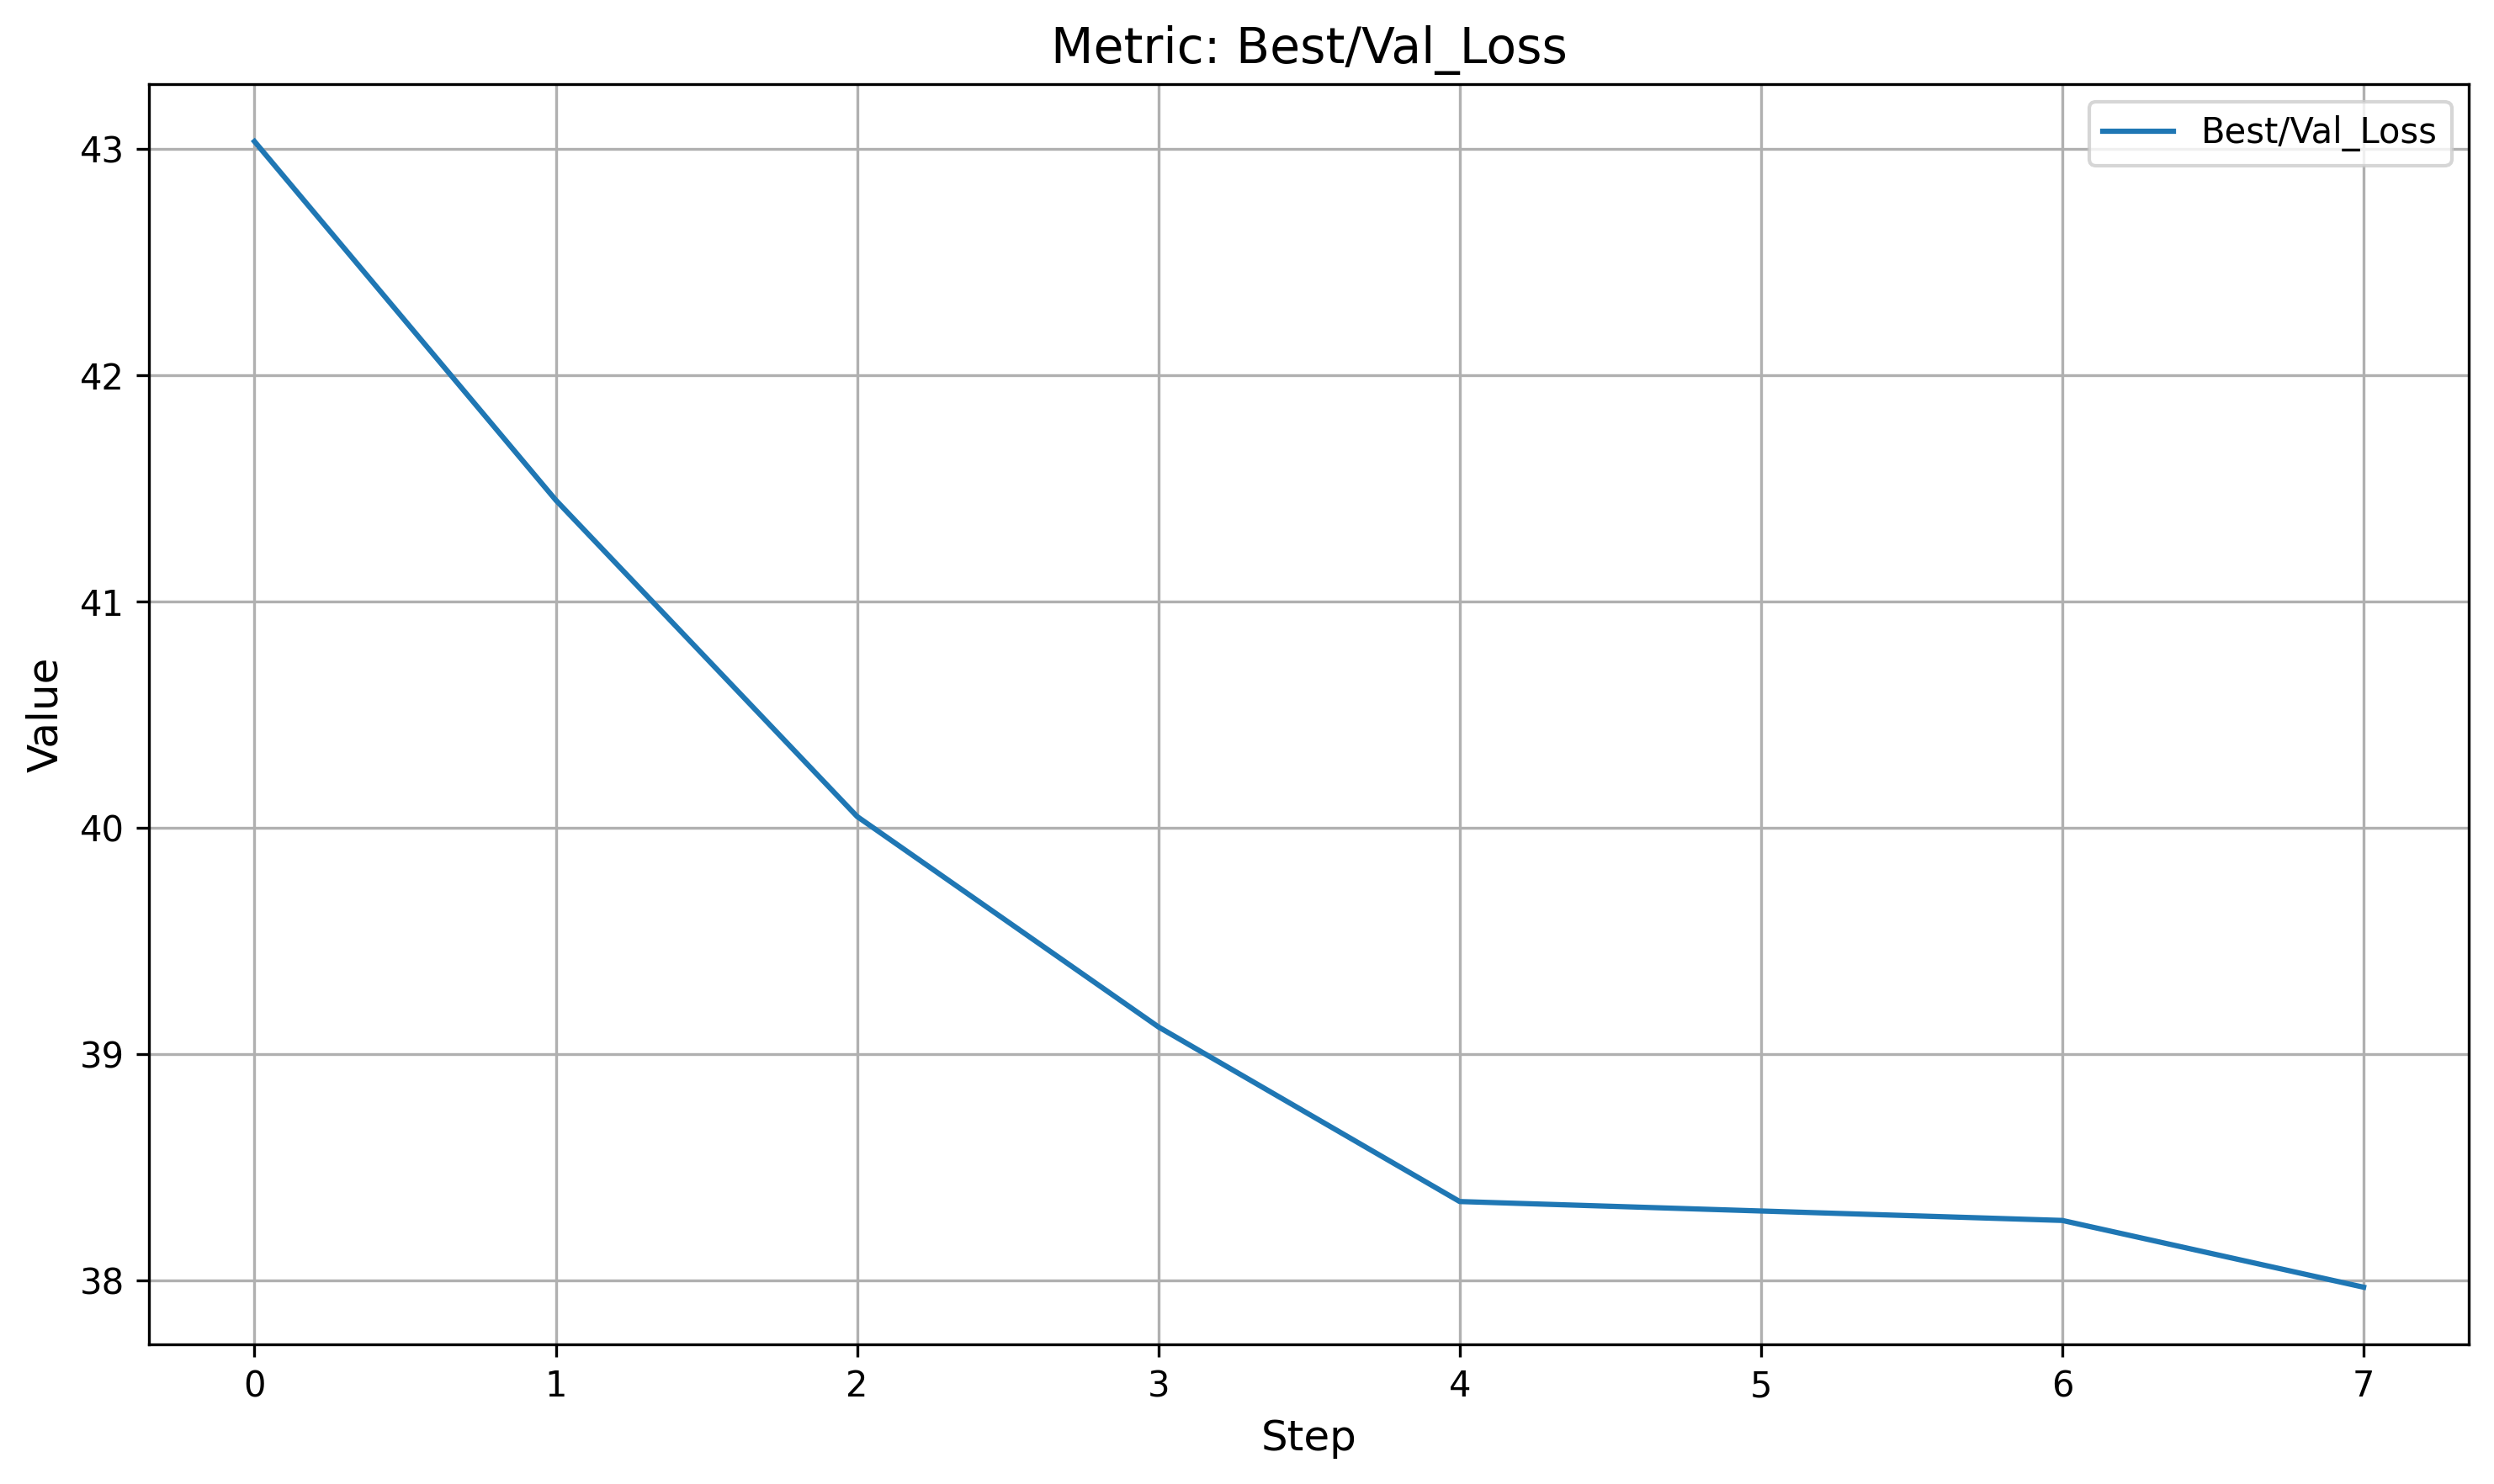
\includegraphics[width=\linewidth]{Images/ASR/Results/shaswot-graphs/BestVal_Loss.png}
	\caption{Best Validation Loss (Cumulative Minimum)}
\end{figure}
The Best Validation Loss (Figure 6-3) is monotonically non-increasing, confirming that the best checkpoint improves over time.
\begin{figure}[H]
	\centering
	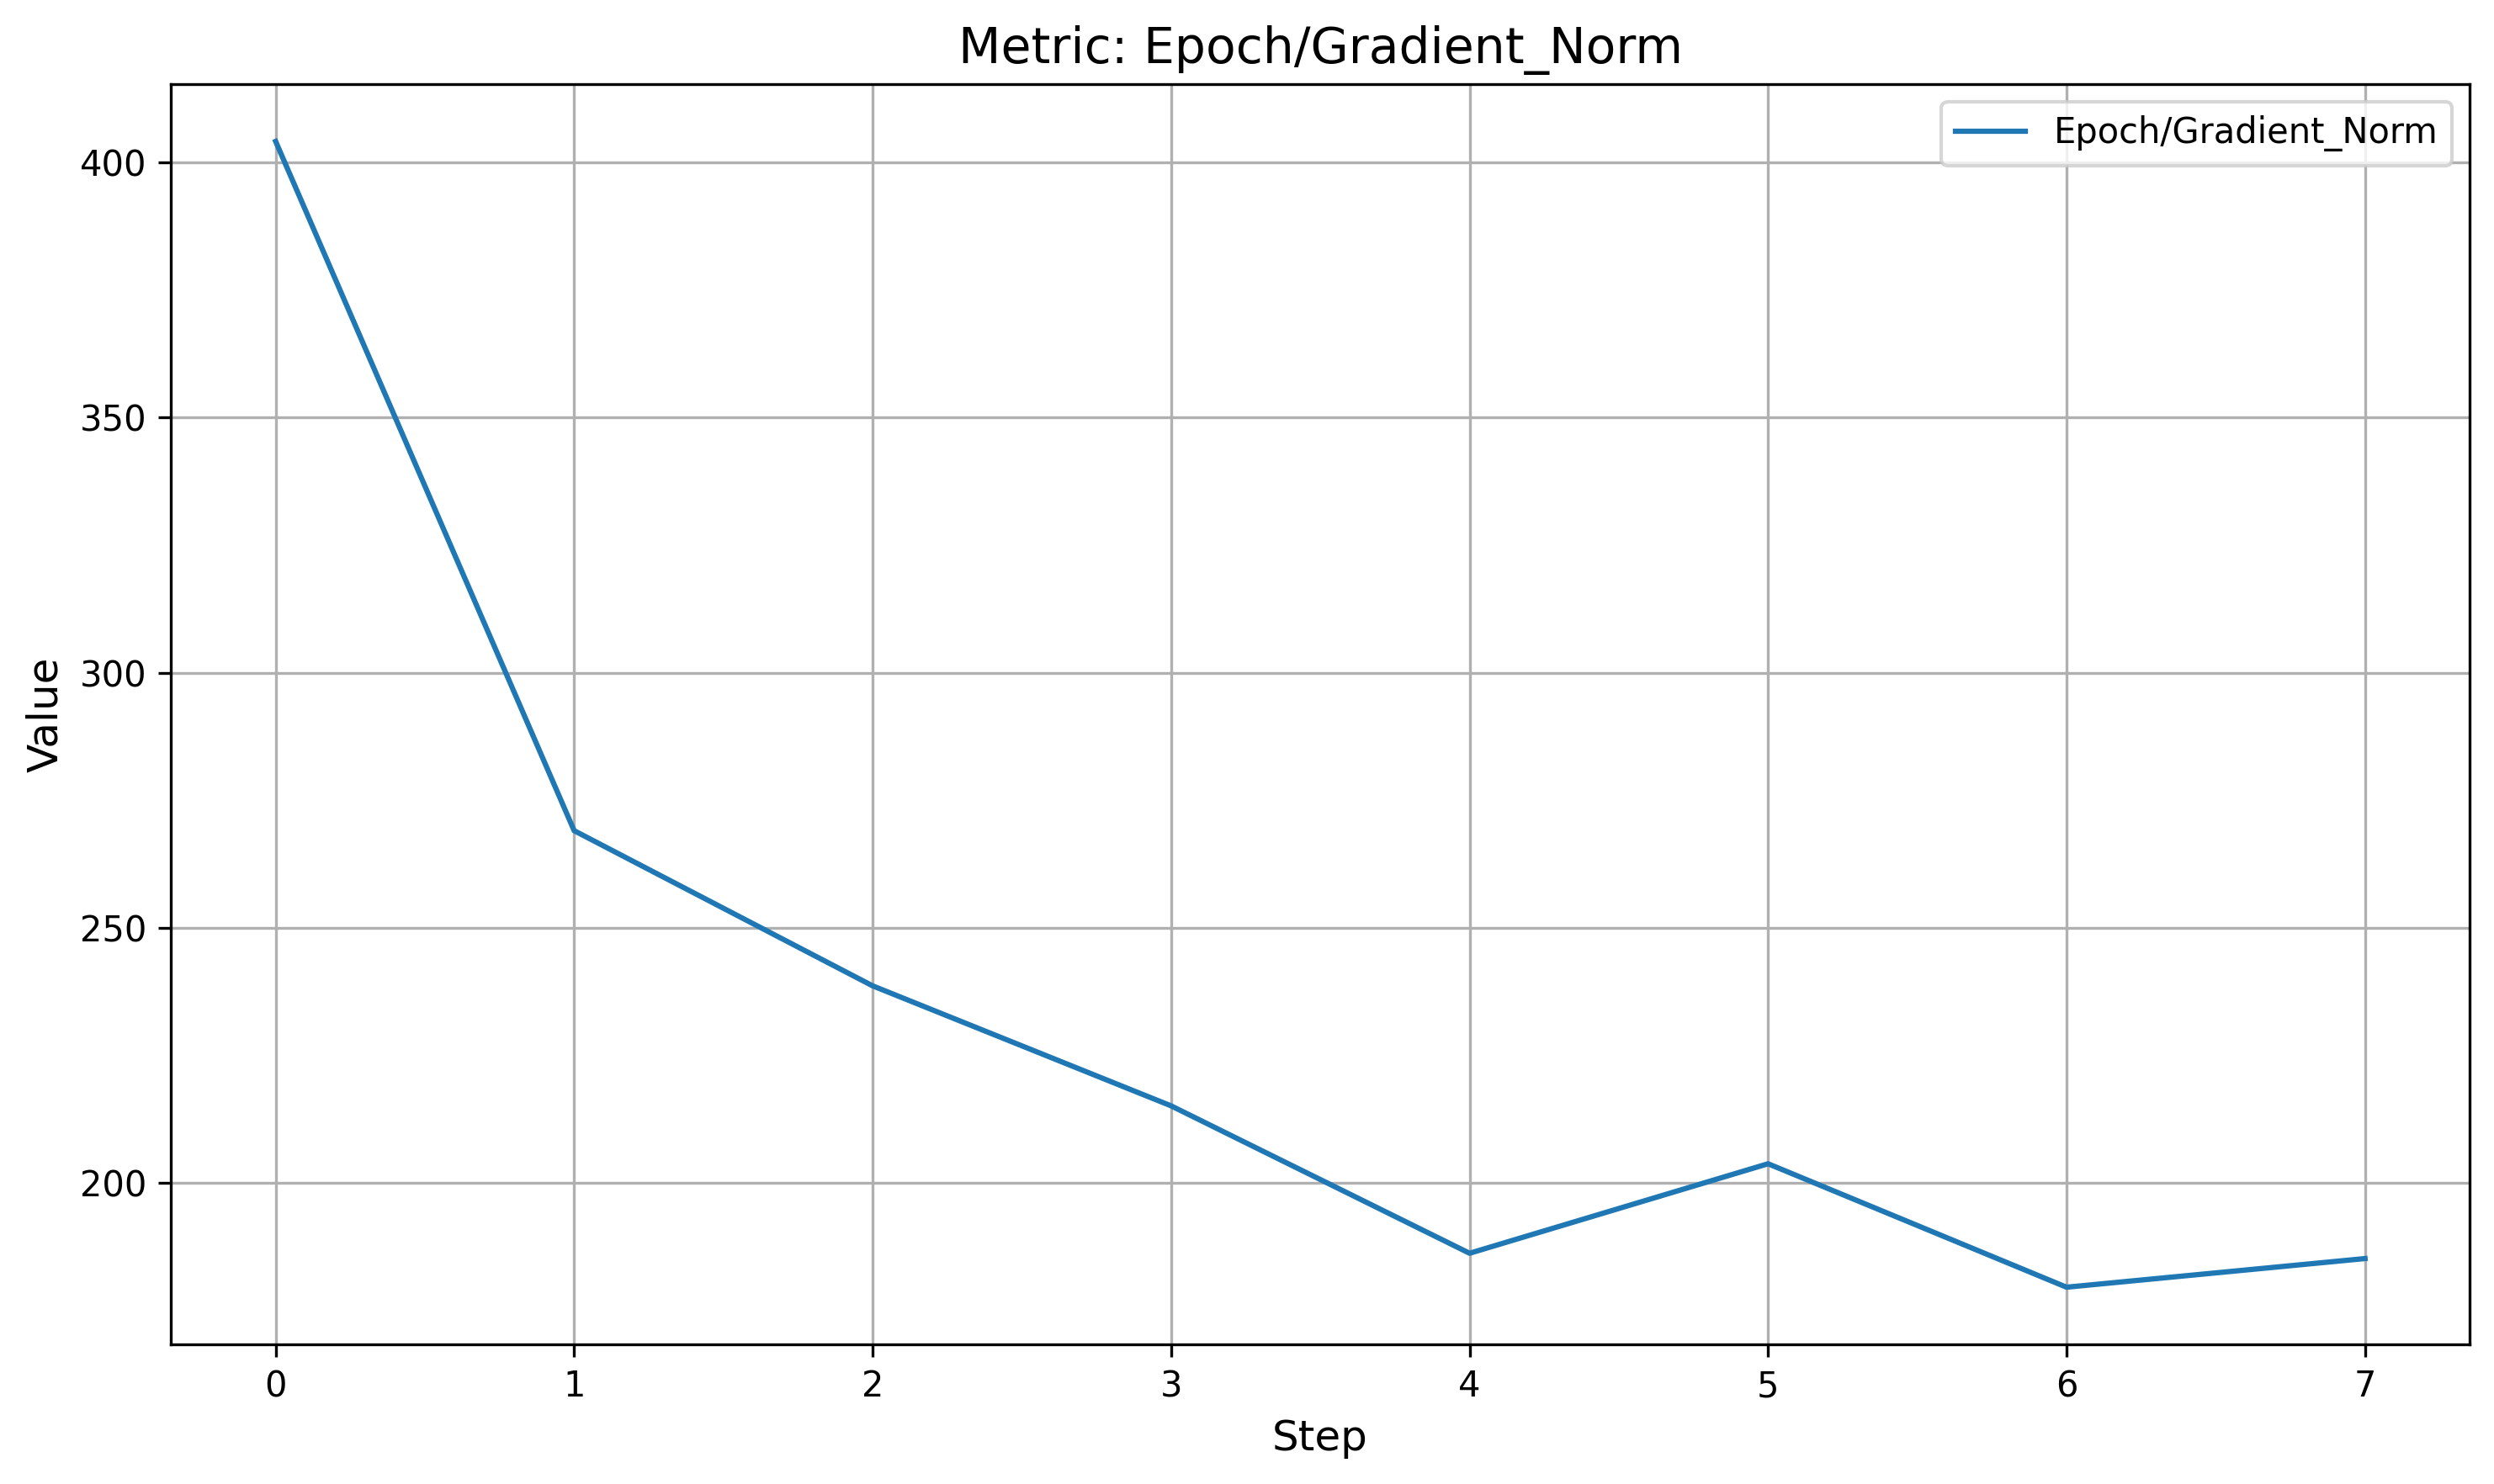
\includegraphics[width=\linewidth]{Images/ASR/Results/shaswot-graphs/EpochGradient_Norm.png}
	\caption{Gradient Norm per Epoch}
\end{figure}
The Gradient Norm (Figure 6-4) drops rapidly in early epochs and stabilizes around 180–185, signaling convergence and stable optimization. Collectively, these curves confirm a stable, well-behaved training process with no signs of divergence or instability.

\subsubsection{Dataset Preperation}
The Automatic Speech Recognition (ASR) datasets are usually based on 16 kHz mono audio due to the effective tradeoff between speech intelligibility and computational efficiency. The 16 kHz sampling frequency, which is based on the Nyquist theorem, retrieves the frequencies up to 8 kHz- the range that is most important to the human voice- without introducing the high-frequency data that is not necessary and beneficial to the recognition performance as offered by higher rates such as 44.1 kHz. Also, mono (single-channel) audio is common in ASR systems since recognition is based on phonemes and time, and not space or direction; downmixing stereo audio to mono reduces memory space by half, makes preprocessing and model construction much easier, and does not lose speech content that is important. Combined, these decisions help to cut down on data size and computational load to support faster and more efficient model training and inference without compromising accuracy.

OpenSLR54, Librispeech100 and OpenSLR12 hosted the dataset which contained the nepali and English audio dataset. The dataset was split into training set, validation set and test set in an 85:10:5 in a data of 10 hours to make sure that there is enough data to be used in the model learning and still have smaller portions to be used in the evaluation and tuning. In an effort of enhancing the strength of the ASR model, noise augmentation was done on each split separately. In particular, each subset consisted of 50\% samples that were randomly selected and noised with the environment. The four categories used in drawing the noise included crowd, construction, traffic, and wind to recreate the acoustic conditions in the real world. The individual clean audio samples were then randomly cross-mixed with a noise segment of these categories using a controlled SNR-based method, so as to guarantee a consistent noise intensity across the dataset. The rest half of the data were retained clean to have a balance in terms of noisy and noise free samples. Through this strategy, the model is able to learn the optimal and negative listening conditions, hence improving its generalization and performance in the real world implementation situations.

The majority of our data was obtained by OpenSLR. The files and its description are contained in manifest. Every sample has a distinct identifier, the audio file path, audio transcription, type of noise, signal to noise ratio in decibels, and dataset division (train, validation, or test). This format is easy to access and filter and is therefore appropriate to use in tasks such as speech recognition in dissimilar acoustic environments. For the purpose of testing independently, We used Fleurs dataset which contains about 2.28 hours of audio data with its transcript. The Fleurs dataset contains the clean audio file and the well-structured transcript for the nepali language. All the audio files here were embedded with noise using scripts with the SNR level similar to the training dataset and the dataset was used specifically for the purpose of testing our model.


\subsubsection{FastConformer-CTC-BPE}

\textbf{Model Architecture and PEFT Configuration}

The NVIDIA NeMo FastConformer-CTC-BPE model was used as the base automatic speech recognition system in the experiments. The model follows an encoder-decoder architecture that uses Connectionist Temporal Classification (CTC) loss for sequence-to-sequence mapping. The encoder is a Conformer-based model with approximately ~ 13 million parameters, while the decoder is a convolutional ASR decoder with 181,000 parameters. The total number of parameters in the base model is 13,204,721.

To achieve parameter-efficient fine-tuning, the NeMo adapter-based PEFT architecture was used. This approach is supported by NeMo as an alternative to LoRA for Conformer-based architectures. Adapter modules were inserted only into the encoder component, while all other parameters were kept frozen during training. Each adapter used a linear bottleneck architecture under the configurations shown in Table~\ref{tab:fastconformer_adapter}. This design reduced the number of trainable parameters to only 50,688, which corresponds to 0.3839\% of the total model parameters.

\begin{table}[H]
\caption{Adapter Configuration Parameters}
\label{tab:fastconformer_adapter}
\centering
\begin{tabular}{|l|l|}
\hline
\textbf{Parameter} & \textbf{Configuration Value} \\
\hline
Target Module & Encoder \\
Adapter Dimension & 8 \\
Adapter Dropout & 0.25 \\
Activation Function & Swish \\
Normalization Position & Pre-norm \\
Input Feature Size & 176 \\
Trainable Parameters & 50,688 \\
Trainable Percentage & 0.3839\% \\
\hline
\end{tabular}
\end{table}

\textbf{Dataset and Preprocessing}

Training was conducted on a custom English ASR dataset written in NeMo manifest format and stored as JSONL files. The dataset was divided into training, validation, and test subsets. All audio samples were processed at a sampling rate of 16,000 Hz. Duration filtering was applied to remove utterances shorter than 0.5 seconds and longer than 20 seconds.

The data loader used seven worker processes with pinned memory enabled to improve GPU data transfer efficiency. Silence trimming was disabled in order to preserve natural speech characteristics. Table~\ref{tab:fastconformer_dataset} presents the statistical distribution of the dataset splits.

\begin{table}[H]
\caption{Dataset Split Statistics}
\label{tab:fastconformer_dataset}
\centering
\begin{tabular}{|l|l|l|l|}
\hline
\textbf{Split} & \textbf{Samples} & \textbf{Duration} & \textbf{Average Words} \\
\hline
Train & 4,859 & 17.03 hours & 35.26 \\
Validation & 571 & 1.99 hours & 35.26 \\
Test & 287 & 0.98 hours & 35.10 \\
\hline
\end{tabular}
\end{table}

\textbf{Training Configuration}

Training was performed using PyTorch Lightning together with the NeMo toolkit. Optimization was carried out using AdamW with decoupled weight decay. A cosine annealing scheduler was used to control the learning rate, together with a warmup phase to stabilize the initial training dynamics. Bfloat16 mixed precision training was enabled to reduce memory usage and accelerate computation on the available GPU hardware. The training hyperparameters are summarized in Table~\ref{tab:fastconformer_train}.

\begin{table}[H]
\caption{Training Hyperparameters}
\label{tab:fastconformer_train}
\centering
\begin{tabular}{|l|l|}
\hline
\textbf{Parameter} & \textbf{Value} \\
\hline
Maximum Epochs & 15 \\
Batch Size & 32 \\
Gradient Accumulation Steps & 2 \\
Learning Rate & $1\times10^{-4}$ \\
Minimum Learning Rate & $1\times10^{-6}$ \\
Weight Decay & $5\times10^{-2}$ \\
Adam Betas & (0.9, 0.98) \\
Warmup Ratio & 0.1 \\
Gradient Clipping & 1.0 \\
Precision & bf-16 mixed\\
Learning Rate Scheduler & Cosine Annealing \\
\hline
\end{tabular}
\end{table}

\textbf{Data Augmentation}

SpecAugment was applied during training to improve model robustness against acoustic variability. This augmentation strategy helps the model generalize better to unseen acoustic conditions by masking selected regions of the spectrogram. The frequency and time masking configurations are shown in Table~\ref{tab:fastconformer_aug}.

\begin{table}[H]
\caption{Data Augmentation Parameters}
\label{tab:fastconformer_aug}
\centering
\begin{tabular}{|l|l|l|}
\hline
\textbf{Augmentation Type} & \textbf{Count} & \textbf{Maximum Width} \\
\hline
Frequency Masks & 2 & 15 frequency bins \\
Time Masks & 6 & 30 time steps \\
\hline
\end{tabular}
\end{table}

\textbf{Regularization and Checkpointing}

Early stopping was based on validation Word Error Rate (WER) as the monitoring metric. Model checkpoints were saved at regular intervals, and the best-performing checkpoint was retained according to validation performance. This strategy helped reduce overfitting and ensured that the best model weights were preserved for final evaluation. The checkpointing and early stopping criteria are given in Table~\ref{tab:fastconformer_ckpt}.

\begin{table}[H]
\caption{Checkpoint and Early Stopping Configuration}
\label{tab:fastconformer_ckpt}
\centering
\begin{tabular}{|l|l|}
\hline
\textbf{Configuration} & \textbf{Value} \\
\hline
Monitor Metric & Validation WER \\
Mode & Minimization \\
Patience & 5 epochs \\
Minimum Delta & 0.0 \\
Save Top K & 1 \\
Checkpoint Frequency & Every 1 epoch \\
\hline
\end{tabular}
\end{table}

\textbf{Evaluation Metrics}

Standard ASR evaluation metrics were used to measure model performance. Word Error Rate (WER) was computed using Levenshtein distance between reference and hypothesis word sequences. Character Error Rate (CER) was calculated using character-level Levenshtein distance. These metrics were evaluated both through the PyTorch Lightning evaluation pipeline and through offline transcription on the validation and test sets. Whitespace was preserved during text normalization so that both metrics could be computed consistently. The model achieved a best validation WER of 3.240\%.

\textbf{Software and Hardware Environment}

A fixed software stack was used to ensure reproducibility of the implementation. All experiments were conducted on Google Colab using an NVIDIA Tesla T4 GPU. Deterministic training was enabled in warn-only mode to account for non-deterministic GPU CTC backward operations while maintaining reproducibility wherever possible. A random seed of 42 was used throughout the experiments. The software and hardware specifications are provided in Table~\ref{tab:fastconformer_env}.

\begin{table}[H]
\caption{Software and Hardware Configuration}
\label{tab:fastconformer_env}
\centering
\begin{tabular}{|l|l|}
\hline
\textbf{Component} & \textbf{Version / Specification} \\
\hline
NVIDIA NeMo Toolkit & 2.4.0 \\
PyTorch Lightning & $\geq$ 2.2.0, $<$ 2.6.0 \\
Python & 3.12 \\
CUDA & 12.8 \\
NumPy & 1.26.4 \\
GPU Accelerator & NVIDIA Tesla T4 \\
Random Seed & 42 \\
\hline
\end{tabular}
\end{table}

\textbf{Model Export and Checkpointing}

After training, the best model checkpoint was exported in multiple formats to support different deployment scenarios. The complete model was saved in NeMo format with full model weights for direct deployment. In addition, the adapter weights were saved separately in PyTorch format, containing only the trainable adapter parameters for efficient storage and transfer. This dual-export strategy supports both full-model deployment and adapter-only fine-tuning in resource-constrained environments.

\subsubsection{Implementation Details for Indic Conformer}

\textbf{Model Architecture and Configuration}

The automatic speech recognition system was built using the IndicConformer \texttt{stt\_ne\_conformer\_ctc\_rnnt\_large} variant. This model uses a hybrid loss function that combines Connectionist Temporal Classification (CTC) and Recurrent Neural Network Transducer (RNNT) objectives, allowing it to benefit from both alignment-free and sequence-to-sequence training paradigms.

The architecture consists of a Conformer-based encoder, an RNNT decoder, a joint network, and an additional CTC decoder head. The model uses a SentencePiece tokenizer with a vocabulary of 5,632 tokens, derived from 256 tokens per language unit. Unlike the FastConformer-CTC-BPE setup, all model parameters were fully fine-tuned, resulting in approximately 129 million trainable parameters. Table~\ref{tab:indic_model} summarizes the main architectural components and their parameter distribution.

\begin{table}[H]
\caption{Model Components and Parameter Distribution}
\label{tab:indic_model}
\centering
\begin{tabular}{|l|l|l|l|}
\hline
\textbf{Component} & \textbf{Module Type} & \textbf{Parameters} & \textbf{Mode} \\
\hline
Preprocessor & AudioToMelSpectrogramPreprocessor & 0 & Train \\
Encoder & ConformerEncoder & 115 M & Train \\
Decoder & RNNTDecoder & 6.9 M & Train \\
Joint Network & RNNTJoint & 4.4 M & Train \\
CTC Decoder & ConvASRDecoder & 2.9 M & Train \\
Loss Functions & RNNTLoss, CTCLoss & 0 & Train \\
\textbf{Total} & -- & 129 M & Train \\
\hline
\end{tabular}
\end{table}

\textbf{Dataset and Preprocessing Pipeline}

The experiments were conducted on a Nepali speech dataset split into training and validation subsets. All audio files were standardized to mono-channel format with a sampling rate of 16,000 Hz. Manifest files were normalized to ensure consistency across transcription-related fields such as \texttt{text}, and \texttt{transcript}, which were mapped to a common format.

No additional audio resampling was applied during fine-tuning, and silence trimming was disabled to preserve natural speech characteristics. Table~\ref{tab:indic_dataset} presents the dataset statistics, including sample counts and duration.

\begin{table}[H]
\caption{Dataset Duration Statistics}
\label{tab:indic_dataset}
\centering
\begin{tabular}{|l|l|l|l|}
\hline
\textbf{Split} & \textbf{Sample Count} & \textbf{Duration (Hours)} & \textbf{Average Duration (Seconds)} \\
\hline
Training & 15,820 & 15.59 & 3.55 \\
Validation & 3,955 & 3.82 & 3.48 \\
\hline
\end{tabular}
\end{table}

\textbf{Training Hyperparameters and Optimization}

The model was fine-tuned using PyTorch Lightning together with the AI4Bharat NeMo fork. AdamW with decoupled weight decay was used as the optimizer. The learning rate schedule followed a WarmupAnnealing strategy with 500 warmup steps followed by annealing. Training was conducted for up to 15 epochs with a batch size of 16 samples per step.

Gradient clipping with a value of 1.0 was applied to stabilize optimization. Early stopping with a patience of 3 epochs was used based on validation WER to reduce overfitting. The full training configuration is given in Table~\ref{tab:indic_train}.

\begin{table}[H]
\caption{Training Hyperparameters}
\label{tab:indic_train}
\centering
\begin{tabular}{|l|l|}
\hline
\textbf{Hyperparameter} & \textbf{Value} \\
\hline
Maximum Epochs & 15 \\
Training Batch Size & 32 \\
Evaluation Batch Size & 64 \\
Gradient Accumulation & 1 \\
Learning Rate & $5\times10^{-5}$ \\
Weight Decay & $1\times10^{-3}$ \\
Warmup Steps & 1000 \\
Gradient Clipping & 1.0 \\
Early Stopping Patience & 5 \\
Early Stopping Min Delta & 0.001 \\
Checkpoint Save Top K & 2 \\
Validation Frequency & Every 1 Epochs \\
\hline
\end{tabular}
\end{table}

\textbf{Regularization and Augmentation}

SpecAugment was used during training to improve robustness against noise and acoustic variability. The implementation used a Numba CUDA kernel for efficient spectrogram masking. The augmentation strategy included both frequency masking and time masking of the input spectrograms.

Brain floating point 16bit (bf16-mixed) was also enabled to reduce memory consumption and speed up computation. Table~\ref{tab:indic_runtime} shows the runtime and optimization settings.

\begin{table}[H]
\caption{Runtime and Optimization Settings}
\label{tab:indic_runtime}
\centering
\begin{tabular}{|l|l|}
\hline
\textbf{Configuration} & \textbf{Setting} \\
\hline
Spectrogram Augmentation & Enabled \\
Augmentation Kernel & Numba CUDA \\
Precision & bf16-mixed\\
Matrix Multiplication Precision & Medium \\
CuDNN Benchmark & Enabled \\
\hline
\end{tabular}
\end{table}

\textbf{Hardware and Software Environment}

All experiments were carried out in Google Colab with high-performance GPU acceleration. The software stack included the AI4Bharat fork of NVIDIA NeMo, patched for compatibility with NumPy 2.x runtimes. Particular attention was given to version compatibility for PyTorch and PyTorch Lightning to ensure reproducibility. The system specifications are shown in Table~\ref{tab:indic_env}.

\begin{table}[H]
\caption{System and Software Specifications}
\label{tab:indic_env}
\centering
\begin{tabular}{|l|l|}
\hline
\textbf{Component} & \textbf{Specification} \\
\hline
GPU & NVIDIA A100-SXM4-80GB \\
CUDA Version & 12.8 \\
PyTorch Version & 2.10.0+cu128 \\
PyTorch Lightning & 2.6.1 \\
NeMo Version & 1.23.0rc0 \\
Python Version & 3.12 \\
NumPy Version & 2.0.2 \\
\hline
\end{tabular}
\end{table}

\textbf{Evaluation Metrics and Checkpointing}

Validation Word Error Rate (WER) and Character Error Rate (CER) were used as the primary performance metrics and were computed every second epoch. The training loop also tracked the individual CTC and RNNT loss components to monitor convergence of both objectives.

Model checkpoints were selected based on the lowest validation WER, and the top two checkpoints were retained for final evaluation. The monitored metrics included training loss, validation loss, and the corresponding CTC and RNNT loss components. The evaluation and checkpointing setup is summarized in Table~\ref{tab:indic_eval}.

\begin{table}[H]
\caption{Training and Evaluation Metrics}
\label{tab:indic_eval}
\centering
\begin{tabular}{|l|l|l|}
\hline
\textbf{Metric} & \textbf{Description} & \textbf{Monitoring Frequency} \\
\hline
Validation WER & Primary Optimization Metric & Every 1 Epoch \\
Validation CER & Secondary Accuracy Metric & Every 1 Epoch \\
Training Loss & Combined CTC and RNNT Loss & Every 5 Steps \\
Validation Loss & Combined CTC and RNNT Loss & Every 1 Epoch \\
Checkpoint Monitor & val\_wer\_eval & Every 1 Epoch \\
Checkpoint Mode & Minimization & Every 1 Epoch \\
Early Stopping & Patience = 5, Min Delta = 0.001 & Checked Every 1 Epoch \\
Checkpoint Saving & Top 2 Model Saved & Based on Validation Metric \\
\hline
\end{tabular}
\end{table}

\subsubsection{Model Exporting and Quantization for Indic Conformer}

The fine-tuned IndicConformer Hybrid CTC/RNNT Large model, containing 129 million parameters, was converted to the Open Neural Network Exchange (ONNX) format using a conversion pipeline based on the NVIDIA NeMo framework. After export, post-training quantization was applied to reduce storage requirements and improve deployment efficiency. The export configuration and quantization strategy are described below.

\textbf{Model Export Configuration (NeMo to ONNX)}

The AI4Bharat fork of NVIDIA NeMo (branch \texttt{nemo-v2}) was used to export the model. Because of the architectural complexity of the Conformer encoder, especially the \texttt{rel\_shift} attention mechanism, the legacy TorchScript-based ONNX exporter was used instead of the newer PyTorch Dynamo exporter in order to avoid symbolic shape-related errors. During export, the decoder head was isolated to ensure compatibility with standard inference engines.

\begin{table}[H]
\caption{Model Export Configuration}
\centering
\begin{tabular}{|l|l|}
\hline
\textbf{Configuration Parameter} & \textbf{Setting / Value} \\
\hline
Source Framework & NVIDIA NeMo (AI4Bharat nemo-v2) \\
Model Architecture & EncDecHybridRNNTCTCBPEModel \\
Export Format & ONNX  \\
Decoder Strategy & CTC \\
Input Tensor & \texttt{audio\_signal} (float32), \texttt{length} (int64) \\
Output Tensor & \texttt{logprobs} (float32) \\
Export Device & CUDA \\
\hline
\end{tabular}
\end{table}

\textbf{Quantization Strategy}

To make the model suitable for deployment in resource-constrained environments, dynamic post-training quantization was applied to the exported FP32 ONNX model. This method converts model weights from floating point to integer representation without requiring a calibration dataset. As a result, the deployment pipeline remains simple while still providing substantial storage savings with acceptable accuracy retention.

\begin{table}[H]
\caption{Quantization Configuration}
\centering
\begin{tabular}{|l|l|}
\hline
\textbf{Quantization Parameter} & \textbf{Setting / Value} \\
\hline
Quantization Library & onnxruntime.quantization \\
Method & Dynamic Quantization  \\
Weight Precision & INT8 \\
Activation Precision & FP32 \\
\hline
\end{tabular}
\end{table}

\textbf{Storage Optimization Results}

The quantization pipeline resulted in a significant reduction in model storage size. Table~\ref{tab:quant_result} compares the original exported model with the quantized version.

\begin{table}[H]
\caption{Model Size Comparison Before and After Quantization}
\label{tab:quant_result}
\centering
\begin{tabular}{|l|l|l|l|}
\hline
\textbf{Model Stage} & \textbf{Precision} & \textbf{File Size (MB)} & \textbf{Size Reduction (\%)} \\
\hline
Indic Conformer & FP32 & 493.05 & --- \\
Exported ONNX & FP32 & 470.22 & 4.6\% \\
Quantized ONNX & INT8 & 133.94 & 71.51\% \\
\hline
\end{tabular}
\end{table}

The quantized implementation reduced the model footprint by approximately 71.5\%, making it more suitable for deployment on edge devices and in environments with limited storage capacity. At the same time, the original inference logic of the architecture was preserved through ONNX Runtime execution.
\subsection{SLM}
\subsubsection{Inference}
\textbf{Before Training}
\begin{itemize}
    \item \textbf{Input text:} What type of cloud is typically associated with thunderstorms?
    \item \textbf{Output:} What type of cloud is typically associated with thunderstorms? imaginaryonetolution Mortgage TT remember gard ACTIONSussedOND repeEdge Storage severerelease
\end{itemize}

\textbf{After loading weights}
\begin{itemize}
    \item \textbf{Input text:} What type of cloud is typically associated with thunderstorms?
    \item \textbf{Output:} What type of cloud is typically associated with thunderstorms? Why did lightning get it going down in Oklahoma?" What sort of cloud was seen on September 19 that led to reports
\end{itemize}

\textbf{After instruction finetuning}
\begin{verbatim}
Below is an instruction that describes a task. Write a response that 
appropriately completes the request.
Rewrite the sentence using a simile.
### Input:
The car is very fast.
Correct response:
>> The car is as fast as lightning.
Model response:
>> The car is as fast as a bullet.
-------------------------------------
Below is an instruction that describes a task. Write a response 
that appropriately completes the request.
### Instruction:
What type of cloud is typically associated with thunderstorms?
Correct response:
Model response:
>> The type of cloud associated with thunderstorms is a cumulus cloud.
-------------------------------------
Below is an instruction that describes a task. Write a response 
that appropriately completes the request.
### Instruction:
Name the author of 'Pride and Prejudice'.
Correct response:
>> Jane Austen.
Model response:
>> The author of 'Pride and Prejudice' is Jane Austen.
\end{verbatim}

\subsubsection{Evaluation Metrics}
\textbf{BLEU Score Analysis}\\
BLEU is a common metric to evaluate machine‐generated text with one or more
reference texts. A single BLEU score calculates precision where zero being the worst and
one being perfect. Typically for NLP tasks, a BLEU4 score of at least 0.4 is
considered good, while a score of 0.6 and higher is exceptional. The comparative analysis of the performance regarding our model shows a relatively low score of 0.3061 for BLEU-4 and 0.45 for BLEU-1 score.

The BLEU-1 score checks for only single word overlaps while the BLEU-2 and higher grams look for matches of 2,3 and 4 word sequences respectively. These are obviously harder to match as generated text doesn't use the same phrasing as the reference texts. This is the reason we see a drop from .45 to .3061 from BLEU-1 to BLEU-4. The descending slope in the graph confirms that matching long sequences is tougher. %Shorter outputs reduce the

\begin{figure}[H]
    \centering
    \includegraphics[width=\linewidth]{Images/SLM/Results/blue.png}
    \caption{BLEU Score}
\end{figure}

\textbf{ROUGE Score Analysis}\\
ROUGE score is another evaluation metric used for NLP and text-generation related tasks. There are various ROGUE metrics like ROUGE-N, ROUGE-L etc. ROUGE-L evaluates the similarity between generated and reference text based on the length of their Longest Common Subsequence (LCS).

\begin{itemize}
    \item \textbf{Precision (0.5965)}
        \begin{itemize}
            \item About 59.65\% of the words that are generated appeared also within the reference in correct order.
            \item High precision indicates the text has correct information but could miss some parts of the reference.
        \end{itemize}    
    \item \textbf{Recall (0.6256)}
        \begin{itemize}
            \item About 62.56\% of the reference text is covered by the generated text
            \item Higher recall indicates the generated text covers most of the reference text
        \end{itemize}   
    \item \textbf{F1 (0.5862)}
        \begin{itemize}
            \item The F1 score balances the precision and recall
            \item Here the 58.62\% means that the generated text is moderately good in terms of the coverage and correctness when it is compared with reference text
        \end{itemize}
\end{itemize}

\begin{figure}[H]
    \centering
    \includegraphics[width=\linewidth]{Images/SLM/Results/rouge.png}
    \caption{BLEU Score}
\end{figure}

\textbf{Evaluation Metrics Table}

\begin{table}[H]
    \centering
    \caption{Evaluation Metrics}
    \begin{tabular}{|l|l|}
        \hline
        Metric & Value\\
        \hline
        Masked Loss & 0.6722 \\
        Perplexity & 1.96\\
        BERTScore F1 & 0.9303\\
        ROUGE-L & 0.5862\\
        \hline
    \end{tabular}
\end{table}

\subsubsection{BLEU vs ROUGE Score}

\begin{figure}[H]
	\centering
	\includegraphics[width=\linewidth]{Images/SLM/Results/blueVsRouge.png}
	\caption{BLEU vs ROUGE scores for different n-grams}
\end{figure}

The scatter plot compares BLEU and ROUGE-F1 scores across three metrics:
BLEU-1 vs. ROUGE-1 (red), BLEU-2 vs. ROUGE-2 (blue), and BLEU-4 vs. ROUGE-L (green). Overall, there is a positive correlation, higher BLEU scores means higher ROUGE scores.

\textbf{Upward Sloping trend}

Each cluster shows an upward trend, which shows the model performing well in BLEU(n-gram precision) also tends to perform well in ROUGE. Points near the diagonal typically show a system where both metrics are balanced. Points above the diagonal indicate a higher ROUGE Score than a BLEU score meaning the model prioritizes concise but incomplete outputs. Similarly, points below the diagonal indicate a higher BLEU score than ROUGE SCORE indicating the model focuses more on recall rather than precision.

\textbf{Differences Among the Clusters}

The orange cluster (BLEU-1 vs. ROUGE-1) is tightly aligned, as both focus on unigram overlap. The blue cluster (BLEU-2 vs. ROUGE-2) shows more variation, reflecting sensitivity to bigram accuracy. The green cluster (BLEU-4 vs. ROUGE-L) is the most dispersed because BLEU-4 requires strict 4-gram matches, whereas ROUGE-L checks the longest
common subsequence which might not align perfectly with exact four-gram overlap.

\subsection{RAG}
\subsubsection{Faithfulness Comparison}
\begin{figure}[H]
	\centering
	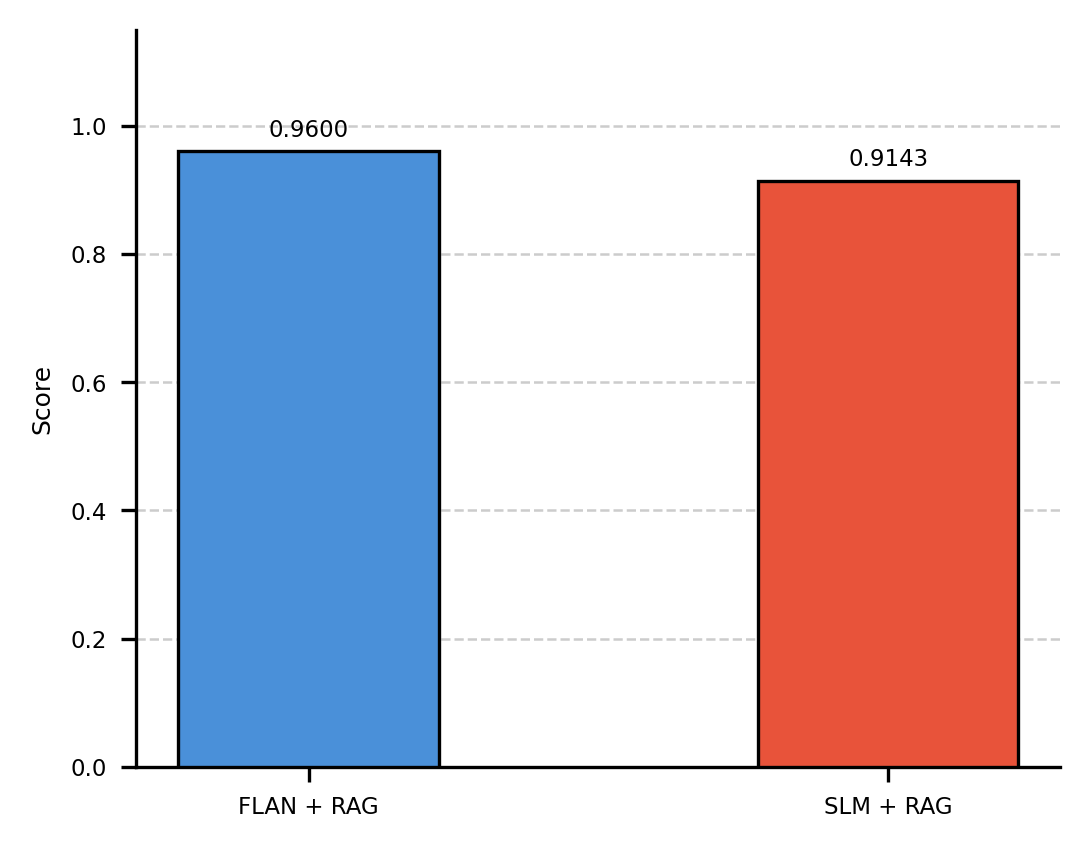
\includegraphics[width=\linewidth]{Images/RAG/Results/rag-faith}
	\caption{Faithfulness scores comparing FLAN + RAG and SLM + RAG configurations.}
\end{figure}

\subsubsection{Answer Relevancy Comparison}
\begin{figure}[H]
	\centering
	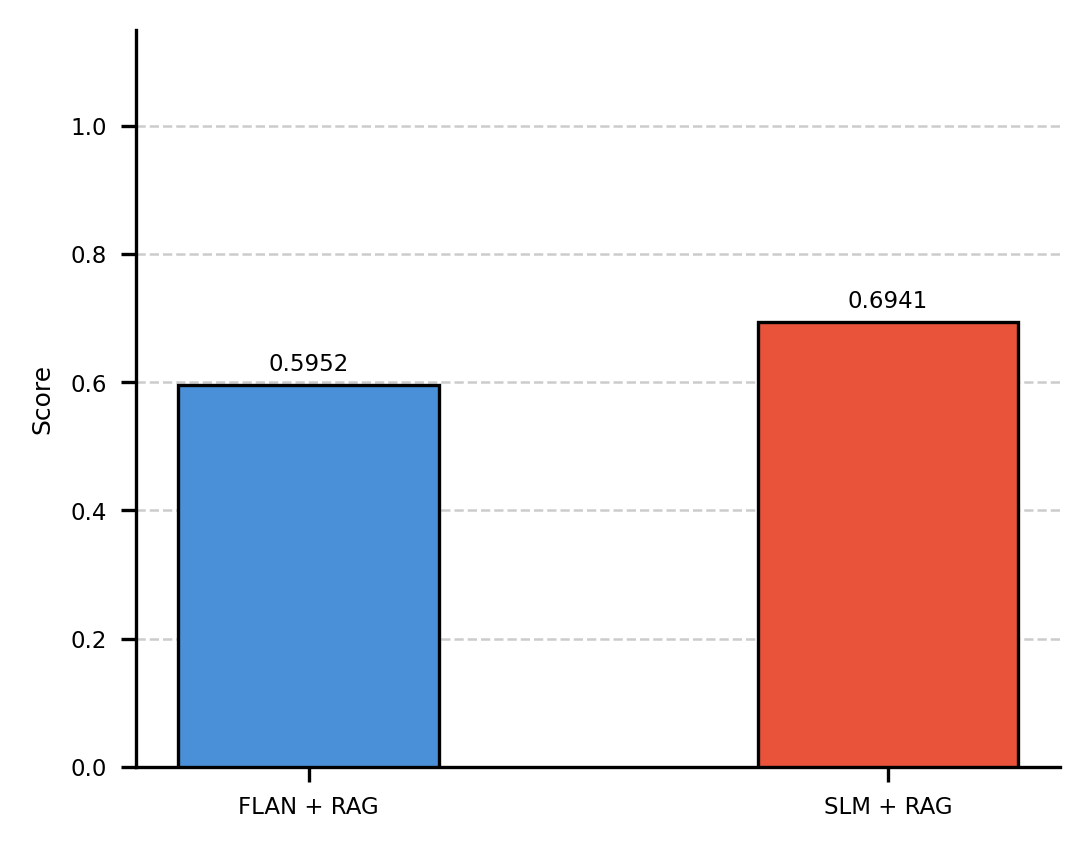
\includegraphics[width=\linewidth]{Images/RAG/Results/rag-answer-relevant}
	\caption{Answer relevance scores comparing FLAN + RAG and SLM + RAG configurations.}
\end{figure}

\subsubsection{RAG Latency Comparison}
\begin{figure}[H]
	\centering
	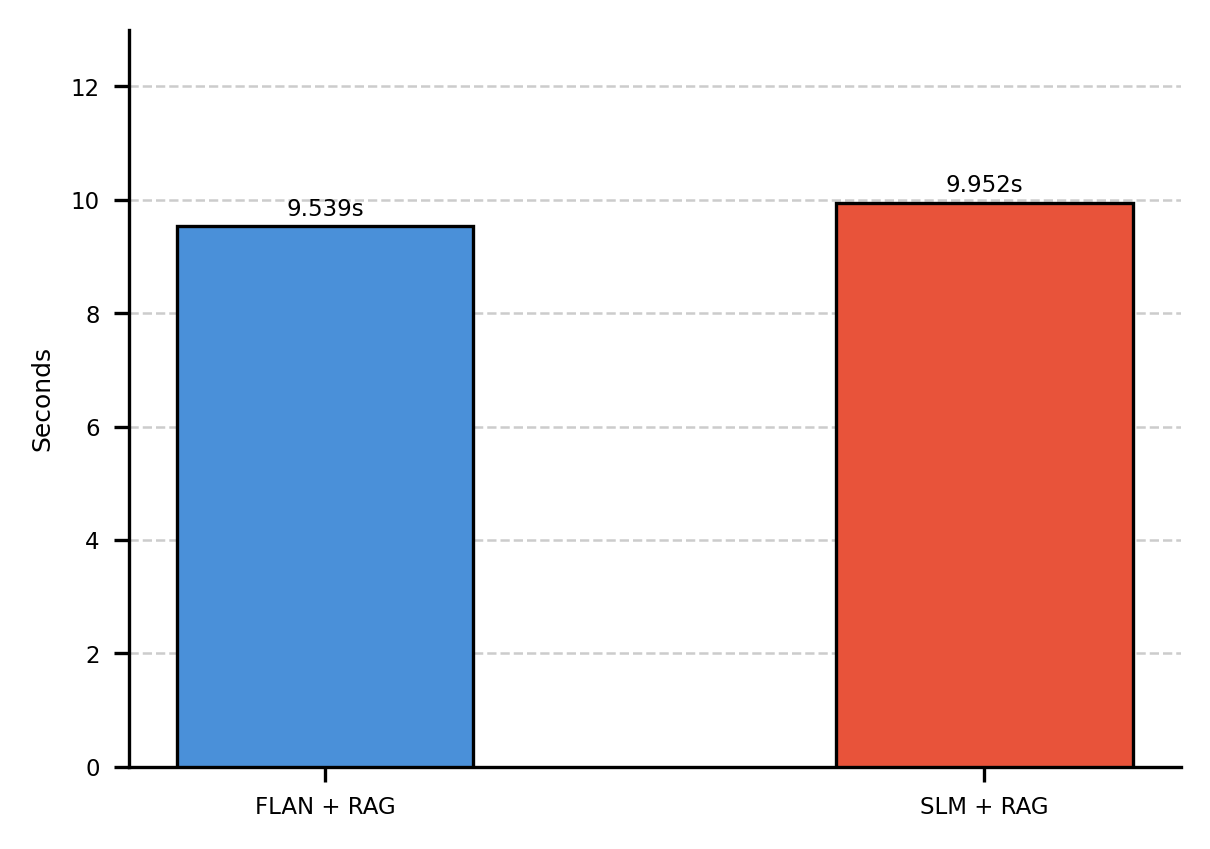
\includegraphics[width=\linewidth]{Images/RAG/Results/rag-latency}
	\caption{Generation latency (seconds) comparing FLAN + RAG and SLM + RAG configurations.}
\end{figure}

\subsubsection{RAG Answer Length Comparison}
\begin{figure}[H]
	\centering
	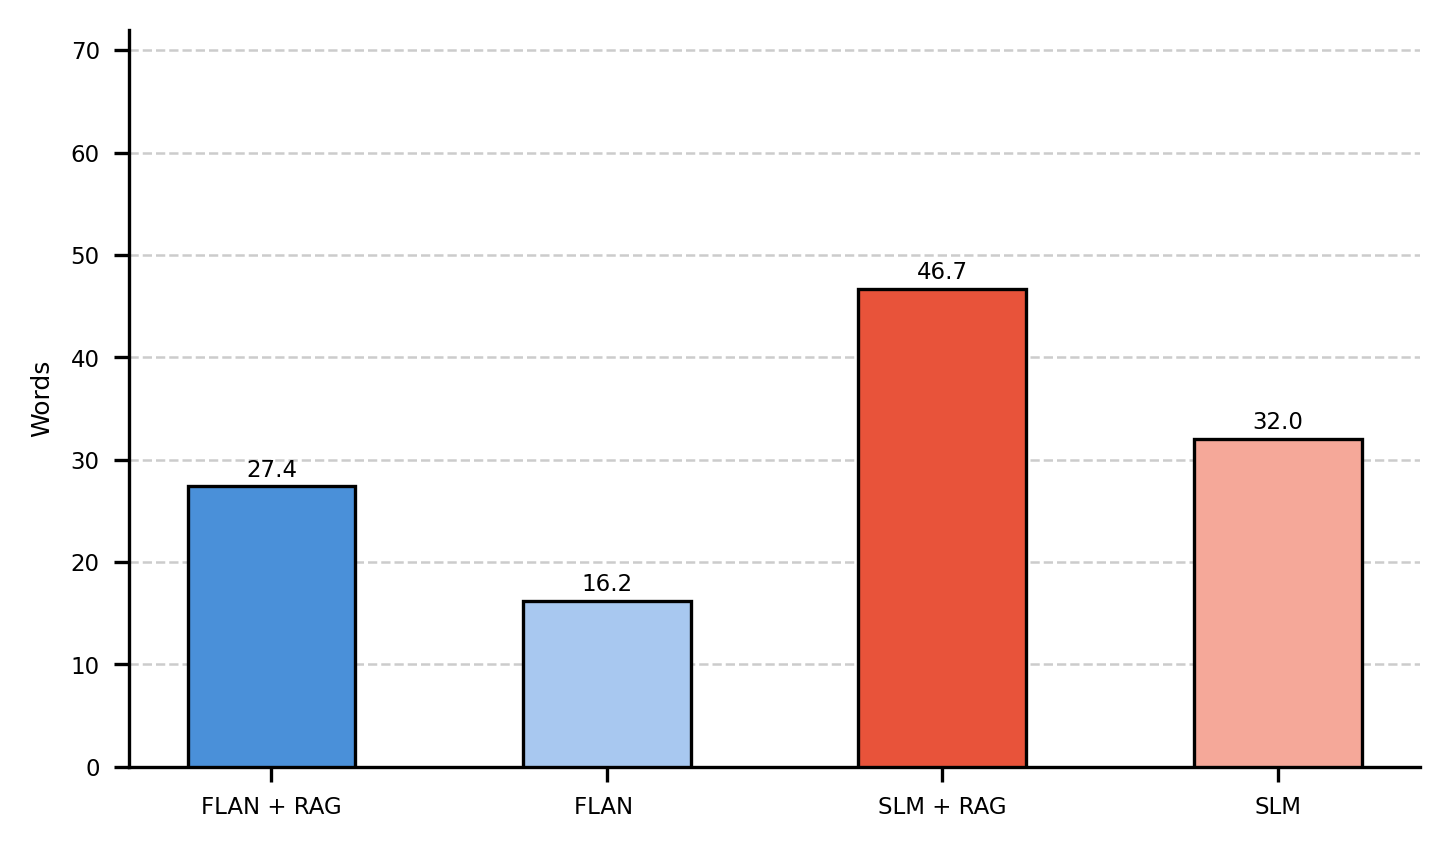
\includegraphics[width=\linewidth]{Images/RAG/Results/rag-answer-length}
	\caption{Average answer length (words) across all four system configurations.}
\end{figure}

\subsubsection{SLM With RAG vs SLM Comparison}
\begin{table}[H]
\caption{SLM + RAG vs SLM (No RAG) -- Selected Answer Comparisons}
\label{tab:rag_comparison}
\centering
\scriptsize
\begin{tabular}{|p{3.5cm}|p{5.5cm}|p{5.5cm}|}
\hline
\textbf{Question} & \textbf{SLM + RAG} & \textbf{SLM (No RAG)} \\
\hline
How has Nepal addressed corruption in recent years? &
Nepal signed UNCAC in 2003, ratified in 2011, and has since completed its first review covering criminalization, law enforcement, and international cooperation chapters. &
The government has addressed corruption in recent years. \\
\hline
What is Nepal's stance on press freedom? &
The FNJ reported press freedom violations tripled in 2025 vs. the prior year, citing journalist impunity, weak media finances, and rising threats to professional and physical safety. &
Nepal's stance on press freedom is that it is an integral part of the international community and should be respected. \\
\hline
What is the current inflation rate in Nepal? &
The CPI inflation rate is 4.45\%, down from 4.64\% in the previous fiscal year, reflecting easing food and fuel prices. &
The current inflation rate in Nepal is 2.5\% per annum. \\
\hline
How has Nepal's economy recovered from COVID-19? &
NRB FY2023/24 data shows gross foreign exchange reserves rose 32.6\% to Rs. 2,041 billion by mid-July 2024, with strong remittance growth and declining inflation. &
The economy has recovered from the impact of the COVID-19 earthquake. \\
\hline
What is the status of Pokhara International Airport? &
The airport officially opened January 1, 2023. The Rs. 22 billion project spans 200 hectares and connects Pokhara directly to international destinations. &
The status of Nepal Pokhara International Airport is as of July 1, 2017. \\
\hline
How is Nepal expanding its internet connectivity? &
Nepal is building a fiber optic link with China Telecom Global to diversify international bandwidth beyond its single India-dependent terrestrial route. &
Nepal is expanding its internet connectivity. \\
\hline
How is Nepal managing deforestation? &
Nepal received \$9.4 million from the World Bank's FCPF for reducing 1.88 million tons of CO\textsubscript{2} under its REDD program in the Terai Arc Landscape. &
The government of Nepal is working to reduce deforestation and protect the environment. \\
\hline
What is Nepal's stance on the Russia-Ukraine conflict? &
Nepal's MoFA formally opposed Russia's use of force, reaffirming UN Charter principles of sovereignty and calling on all parties to exercise maximum restraint. &
The Nepal government is neutral on the conflict in Ukraine. \\
\hline
How is Nepal participating in UN peacekeeping missions? &
Nepal has participated since 1958, serving in 42 UN missions. It is the 6th largest contributor with 4,834 personnel deployed worldwide, including 130 women. &
Nepal is participating in UN peacekeeping missions. \\
\hline
What is Nepal doing to reduce child marriage? &
Nepal endorsed a National Strategy to End Child Marriage and ran a 2017--2021 nationwide campaign targeting SDGs 5.3 and 16.2, launched by President Bhandari. &
Nepal is doing a great job of reducing child marriage. However, it is important to note that child marriage is a global problem. \\
\hline
\end{tabular}
\end{table}
\newpage
\section{\MakeUppercase{Future Enhancement}}
\newpage
\section{\MakeUppercase{Conclusion}}

The aim of this project was to design and implement a modular bilingual speech-to-dialogue pipeline, which separates the functionality of standard components of a conversational AI system such that each module can be built, optimised, and swapped out independently. The findings achieved across all components confirm this architectural design, and that an intelligently written modular system can provide competitive performance without compromising either flexibility or maintainability.

An English ASR model based on the FastConformer-CTC-BPE architecture, fine-tuned using parameter-efficient adapter modules, attained a WER of 6.14\% on the test set, an impressive result given that only 0.38\% of the total model parameters were updated during fine-tuning. This supports the finding that PEFT-based adaptation of pre-trained Conformer models is a viable and resource-efficient approach to domain-specific ASR. The Nepali ASR, built on the fine-tuned Quantized Indic Conformer, achieved a WER of 31.40\% on the clean FLEURS test set, outperforming all evaluated Whisper variants despite having fewer parameters. Under noisy conditions, the model attained a WER of 33.75\%, demonstrating meaningful noise robustness. The ONNX variant with quantisation further compressed the model to 133.94~MB, making it sufficiently compact for resource-constrained deployment at an acceptable accuracy trade-off.

The small language model, a self-trained decoder-only Transformer, achieved a perplexity of 1.96, a BERTScore-F1 of 0.9303, and a ROUGE-L of 0.5862, indicating that the model is both lightweight and capable of producing semantically coherent and contextually appropriate responses. RAG integration using a FAISS-backed knowledge base of recent news and events significantly improved the factual grounding and relevance of answers generated by the SLM in isolation, directly addressing the hallucination and knowledge staleness inherent to parametric language models trained on fixed datasets.

Together, the bilingual ASR pathways, the RAG-enhanced SLM, and the parallel English and Nepali text-to-speech modules form a complete, end-to-end spoken dialogue system capable of accepting speech in either language and returning contextually relevant, up-to-date spoken responses in the user's preferred language. The system addresses a genuine gap in conversational AI accessibility for Nepali-speaking users and demonstrates that low-resource Indic languages can be effectively integrated into a production-focused pipeline through careful model selection, fine-tuning, and quantisation.

The modular design philosophy adopted in this project represents one of its most significant strengths. Decoupling the components allowed the ASR models to be fine-tuned independently, the knowledge base to be updated without retraining any model, and each stage to be evaluated in isolation. This architecture is conducive to continuous improvement: as stronger alternatives emerge, individual components can be replaced without requiring a full system retraining.

In conclusion, this project demonstrates that a well-structured, decoupled, modular pipeline is not only architecturally sound but also practically viable, delivering strong quantitative performance across ASR, language modelling, and retrieval, while remaining flexible, maintainable, and extensible for future development in real-world multilingual conversational AI applications.

\input{Report/8_Appendices}

% No-cites Here
\nocite{cif}
\nocite{streaming-trans-nobeam}
\nocite{streaming-trans}
\nocite{sangam-book}
\nocite{bert}
\nocite{wav2vec}
\nocite{espnet}
\nocite{macaron}
\nocite{speechLLM}
\nocite{attentionneed}
\nocite{alpaca}
\nocite{slim}
\nocite{laco}
\nocite{ablation}
\nocite{layerwise}

% References (IEEE style)
\newpage
\printbibliography
\addcontentsline{toc}{section}{\MakeUppercase{References}}

\end{document}
